\chapter{Teste Baseado em Modelos para LPS: um Mapeamento Sistemático da Literatura}
\label{sec:secmsl_MSL}
\pagestyle{plain}

\section{Planejamento do MSL}
\label{sec:secmsl_planejamentosml}
\subsection{Objetivo da Pesquisa}
O objetivo deste mapeamento sistemático da literatura é identificar estudos sobre Teste Baseado em Modelo (TBM) para Linha de Produto de Software (LPS) com foco em variabilidade, domínio de aplicação, ferramenta, modelos de LPS, entre outros.

A MSL apresentada aqui segue padrões definidos como principais orientações para a execução de um mapeamento sistemático da literatura por \citet{kitchenham2004procedures} e \citet{keele2007guidelines}.

\section{Metodologia de Pesquisa}
\label{sec:sec_mslmetodologia}

Elaboramos a metodologia de pesquisa seguindo as diretrizes de \citet{petersen2015guidelines} e \citet{kitchenham2015evidence}.

A \ref{fig:mapping_process} mostra a visão geral do nosso processo de mapeamento sistemático.

\begin{figure} [!h]
	\centering
	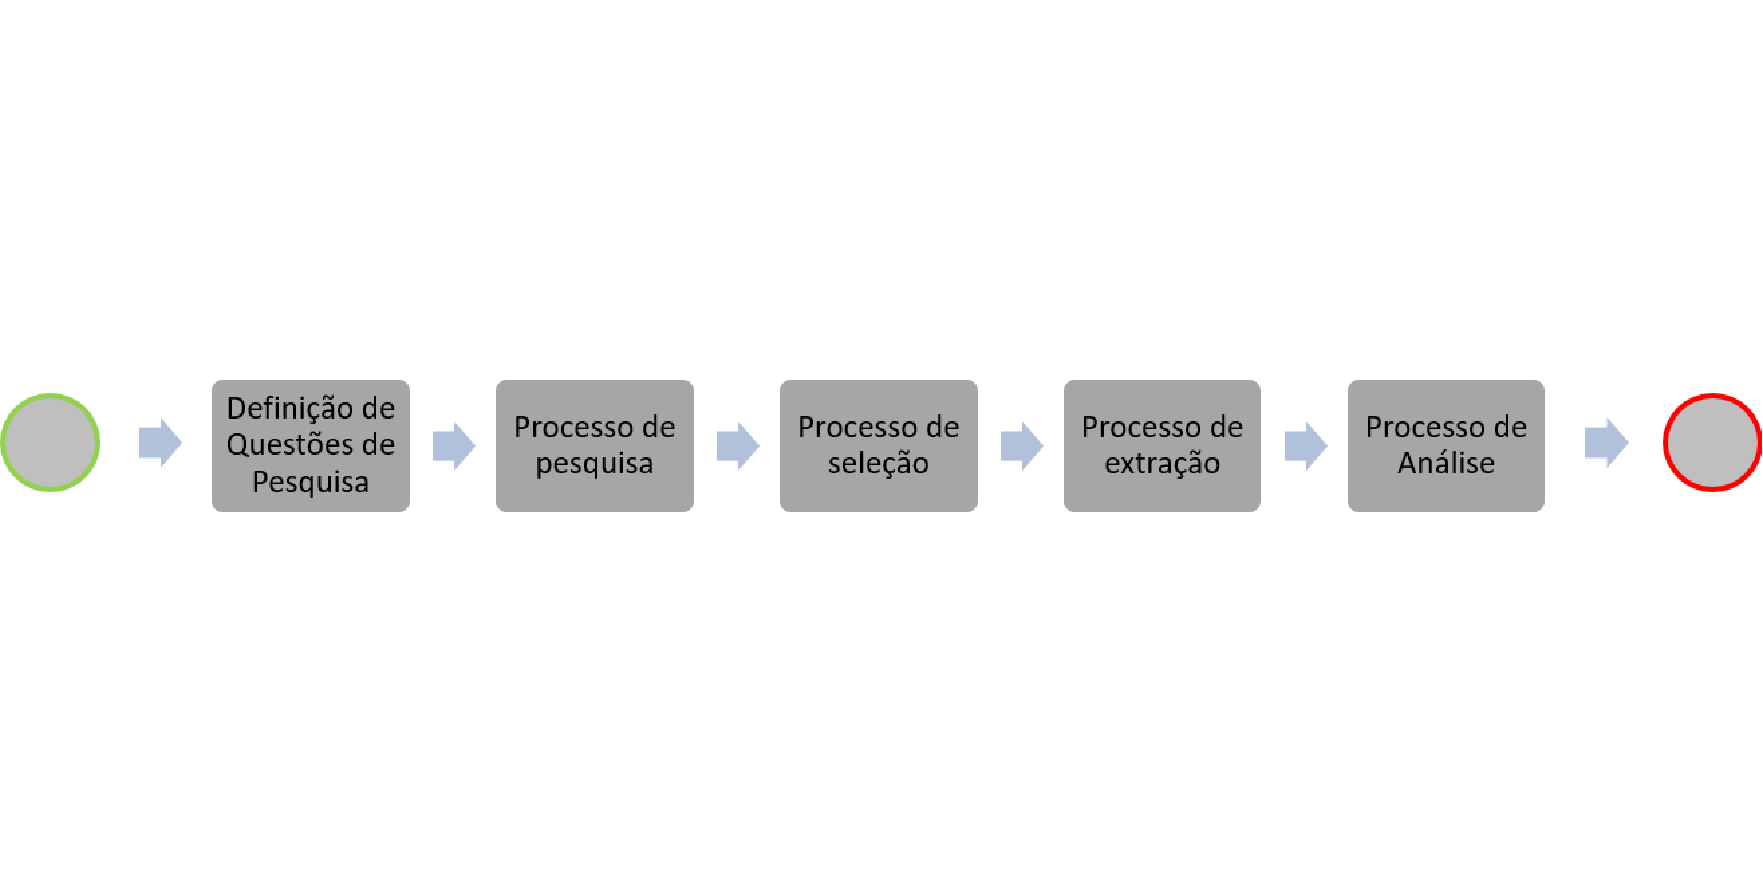
\includegraphics[scale=0.50]{sm_process.pdf}
	\caption{Visão geral do processo de mapeamento sistemático}
	\label{fig:mapping_process}
\end{figure}

Começamos nosso estudo definindo questões de pesquisa (Seção \ref{sec:secmsl_objetivos_equestao}). Em seguida, realizamos o processo de pesquisa (Seção \ref{sec:search_process}) para reunir um conjunto inicial de estudos primários de várias fontes diferentes. Com este conjunto de estudos, realizamos o processo de seleção (Seção \ref{sec:selection_process}), filtrando estudos de acordo com diferentes critérios. O processo de extração (Seção \ref{sec:extraction_process}) foi realizado nos estudos filtrados para suportar o processo de análise. Não processo de análise (Seção \ref{sec:analysis_process}) respondemos as questões de pesquisa definidas para este estudo.


\subsection{Objetivo e Questões de Pesquisa}
\label{sec:secmsl_objetivos_equestao}

Este MSL \textbf{tem como objetivo} coletar evidências da literatura, \textbf{com o propósito de} caracterizar Testes Baseados em Modelo, \textbf{com relação a} sua aplicação em Linhas de Produto de Software, \textbf{do ponto de vista de} Pesquisadores de LPS, \textbf{no contexto de} diferentes fontes digitais de estudo primário.

Nós formulamos seis questões de pesquisa com base no objetivo principal deste MSL, como segue:

\begin{itemize}
	
	\item \textbf{RQ.1: Para quais domínios do aplicativo LPS, tipos de solução e propostas o TBM é usado?}% 1 + 3 + 11
	Estamos interessados em reunir evidências de quais domínios de LPS são mais frequentes, como, por exemplo, software, aeroespacial e automotivo, bem como que tipo de soluções foram propostas para TBM de LPSs;
	
	\item \textbf{RQ.2: Quais abordagens de TBM, níveis de teste e artefatos foram usados para testar LPSs?} Nesta questão, o foco principal é identificar técnicas de TBM, níveis de teste e automação de teste;
	
	\item \textbf{RQ.3: Como a variabilidade e o tempo de ligação são tratados durante o TBM das LPSs?}% 4 + 8
	Nesta questão, gostaríamos de compreender quais estudos primários levam em conta a variabilidade e como eles realizam o gerenciamento da variabilidade nas atividades de TBM da LPS, bem como se o tempo de ligação afeta as atividades do TBM nas LPSs;
	
	\item \textbf{RQ.4: O TBM suporta testes de requisitos não-funcionais de LPS?} Estamos interessados em coletar evidências se os estudos primários dependem do teste de requisitos não-funcionais de LPS;
	
	\item \textbf{RQ.5: Como as propostas de TBM de LPS são avaliadas?} As soluções de TBMs de LPSs devem ser avaliadas como um meio de fornecer evidência de sua viabilidade. Portanto, gostaríamos de entender que tipo de avaliação é realizada, como experimentos controlados e estudos de caso;
	
	\item \textbf{RQ.6: Como a rastreabilidade é considerada durante atividades de TBM para LPSs?} Rastreabilidade é um conceito fundamental de TBM e LPS. Nesta questão, reunimos evidências de como as soluções consideram tal conceito para atividades de TBM em LPS.
	
\end{itemize}

\subsection{Processo de Pesquisa}
\label{sec:search_process}

A \ref{fig:search_process} mostra o processo de busca do MSL.

\begin{figure} [!h]
	\centering
	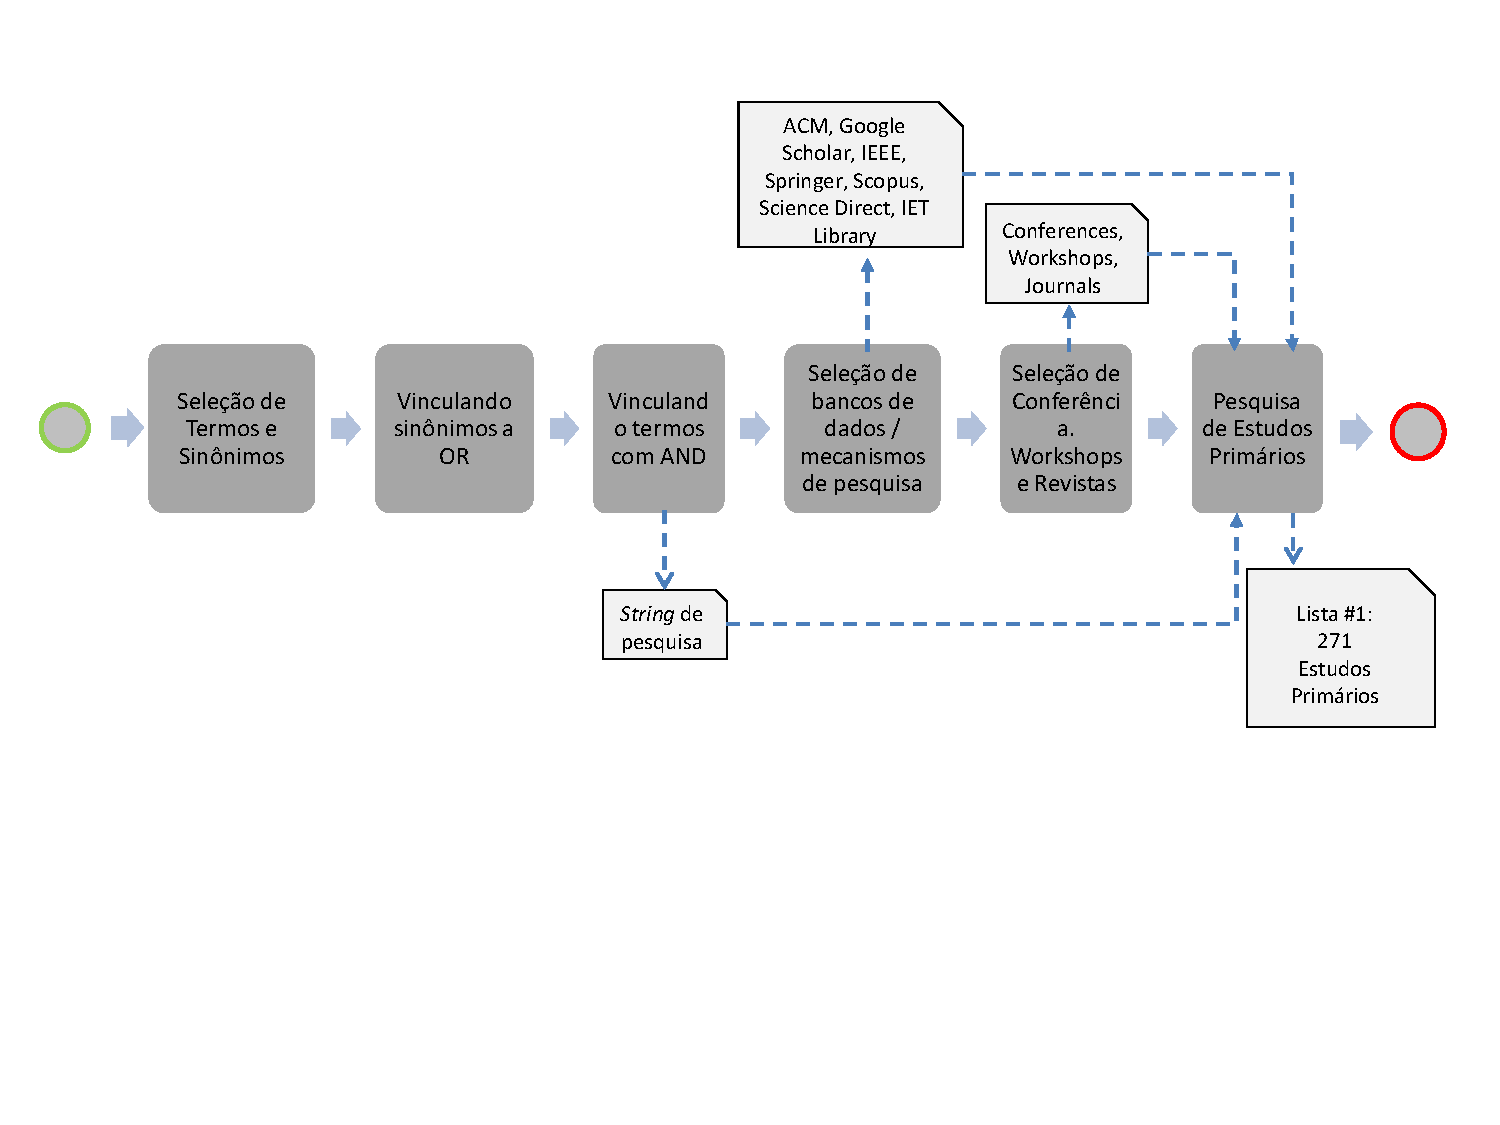
\includegraphics[scale=0.55]{search_process.pdf}
	\caption{Processo de pesquisa por MSL}
	\label{fig:search_process}
\end{figure}

A estratégia de busca para encontrar estudos primários relevantes definidos para este MSL é baseada principalmente na seleção de termos e sinônimos relacionados ao TBM aplicado ao LPS. Esses termos e sinônimos levam em consideração algumas das palavras-chave de trabalhos relacionados e são apresentadas da seguinte forma:

\begin{itemize}
	\item \textbf{\textit{software}};
	\item \textbf{\textit{product line}}:\textit{product-line}, \textit{product family}, \textit{product-family}, \textit{product-families}, \textit{family of products};
	\item \textbf{\textit{model-based testing}}:\textit{model based testing}, \textit{TBM}.
\end{itemize}

Uma vez que tivemos esses termos e seus sinônimos, associamos esses sinônimos ao operador lógico `` OR '' e termos com `` AND ''. Assim, criamos nossa \textit{string} de pesquisa geral, conforme apresentado na \ref{tab:search_string}.

\begin{table}[!h]	
	\centering
	\caption{String de pesquisa geral do MSL}
	\label{tab:search_string}
	\begin{tabular}{@{}c@{}}	
		\hline			
		software \textbf{AND} (``product line'' \textbf{OR} ``product-line'' \textbf{OR} \\``product family'' \textbf{OR} ``product-family'' \textbf{OR} ``product-families'' \textbf{OR} \\``family of products'' \textbf{OR} variability) \textbf{AND} (``model-based testing'' \textbf{OR} \\``model based testing'' \textbf{OR} TBM)	
		\\\hline
	\end{tabular}
\end{table}

Além disso, selecionamos fontes de pesquisa (eletrônica e manual), idioma dos estudos primários e tipo de publicação da seguinte forma:

\begin{itemize}
	\item \textbf{Fontes de Pesquisa:} bases de dados eletrônicas indexadas (IEEE, ACM, ScienceDirect, Scopus, Biblioteca TET IET, Google Scholar, Springer) listadas na \ref{table:fontes} e pesquisa manual em revistas especializadas, conferências e workshops como na \ref{table:conferences} e \ref{table:journals};
	
	\item \textbf{Linguagem de Estudos:} Inglês, devido à sua abrangência na área de Ciência da Computação;
	
	\item \textbf{Tipo de Publicação:} estudos primários revisados por pares publicados em periódicos, conferências / workshops ou capítulos de livros.
\end{itemize}

As razões para escolher essas fontes de pesquisa estão listadas:

\begin{itemize}
	\item fonte de ciência da computação mundialmente conhecida;
	\item fornece um mecanismo de pesquisa avançado capaz de lidar com consultas avançadas;
	\item indexado internacionalmente;
	\item índices de origem conferências e periódicos mais relevantes em Engenharia de Software;
	\item índices de fontes de artigos com fator de alto impacto (JCR e / ou índice H);
	\item Fonte não cessou a publicação.
\end{itemize}

\begin{table}[!h]
	\centering
	\scriptsize
	\caption{Fontes de pesquisa eletrônicas definidas}
	\label{table:fontes}
	\begin{tabular}{l|l}
		\hline \hline
		\textbf{Fonte Eletrônica} & \textbf{URL}                               							\\\hline
		ACM Digital Library  & \url{http://dl.acm.org}                                         \\\hline
		IEEE Xplore          & \url{http://ieeexplore.ieee.org}                                \\\hline
		ScienceDirect        & \url{http://www.sciencedirect.com}                              \\\hline
		Scopus               & \url{http://www.info.sciverse.com/scopus}                       \\\hline
		Springer             & \url{http://www.springer.com}                                   \\\hline
		Google Scholar       & \url{https://scholar.google.com}                                 \\\hline
		IET  Digital Library & \url{http://digital-library.theiet.org/content/journals/iet-sen} \\\hline
		\hline
	\end{tabular}
\end{table}

\begin{table}[!h]
	\centering
	\scriptsize
	\caption{Conferências Definidas e Workshops para Pesquisa Manual}
	\label{table:conferences}
	\begin{tabular}{l|l}
		\hline \hline
		\textbf{Acrônimo} & \textbf{Conferência/Workshop}                                 \\\hline
		ICECCS         & Engineering of Complex Computer Systems                        \\\hline
		AISE           & Advanced Information Systems Engineering                       \\\hline
		ICST           & International Conference on Software Testing                   \\\hline
		ICIS           & Computer and Information Science                               \\\hline
		ACM SIGSOFT    & Software Engineering Nãotes                                     \\\hline
		MSIS           & Workshop on Variability Modeling of Software-Intensive Systems \\\hline
		ILPS           & International Software Product Line Conference                 \\\hline
		ICSTSS         & International Conference on Testing Software and Systems       \\\hline
		QA\&TEST       & International Conference on Software QA and Testing            \\\hline
		IFIP           & International Conference on Testing Software and Systems       \\\hline
		\hline
	\end{tabular}
\end{table}

\begin{table}[!h]
	\centering
	\scriptsize
	\caption{Diários Definidos para Pesquisa Manual}
	\label{table:journals}
	\begin{tabular}{l|l}
		\hline \hline
		\textbf{Acrônimo} & \textbf{\textit{Journal}}                    \\\hline
		STVR					 & Software Testing, Verification \& Reliability \\\hline
		ESE            & Empirical Software Engineering      \\\hline
		JSS            & Journal of Systems and Software     \\\hline
		IST            & Information and Software Technology \\\hline
		ASC            & Applied Soft Computing              \\\hline
		SQJ            & Software Quality Journal            \\\hline
		SCP            & Science of Computer Programming     \\\hline
		\hline
	\end{tabular}
\end{table}

Como última atividade do processo de busca, realizamos a busca por estudos primários aplicando a string de busca a fontes eletrônicas, e buscando estudos primários manualmente em congressos, workshops e periódicos, conforme apresentado nas próximas seções. Um total de 271 estudos (Lista \# 1) foram recuperados no final deste processo.

\subsubsection{Avaliação de protocolo}

Elaboramos um questionário \footnote{\url{https://drive.google.com/open?id=1U0zfLS6JLfO6krrFkbpwL0mflCtrNkVBJ5cGKDjWfJw}} para avaliar nosso protocolo MSL para coletar a opinião de pesquisadores que trabalharam com TBM e / ou LPS, para facilitar a construção da pesquisa. O questionário é composto por oito itens, sete questões em escala de Likert \cite{li2013novel} e uma questão aberta, como segue:

\begin{enumerate}
	\item Este estudo baseia-se em uma importante questão de pesquisa em \textit{Model-Based Testing} (TBM) de linhas de produto de software (LPS).
	\item A cadeia de pesquisa é adequadamente derivada das questões de pesquisa.
	\item As fontes de pesquisa definidas são suficientes para cobrir estudos relevantes.
	\item Os critérios de inclusão e exclusão são adequados e adequadamente descritos.
	\item A pesquisa pode avaliar a qualidade / validade dos estudos selecionados.
	\item O processo de extração aborda adequadamente as questões de pesquisa.
	\item O processo de análise é apropriado para responder às questões de pesquisa.
\end{enumerate}

Cada pergunta do tipo likert tem as seguintes opções como respostas:

\begin{itemize}
	\item \textbf{Eu discordo totalmente:} quando o protocolo não atende aos critérios da pergunta de forma alguma;
	\item \textbf{Discordo Parcialmente} quando o protocolo não atende a alguns critérios da questão;
	\item \textbf{Neutro:} quando o protocolo não deixa claro se ele atende ou não aos critérios da questão;
	\item \textbf{Eu Concordo Parcialmente} quando o protocolo atende a alguns critérios da questão; e
	\item \textbf{Eu concordo plenamente:} quando o protocolo atende totalmente aos critérios da pergunta.
\end{itemize}

para os pesquisadores anotarem onde quer que julguem importante sobre o protocolo

Na parte inferior do questionário, uma opção foi disponibilizada para sugestões gratuitas sobre melhorias do protocolo. O objetivo principal desta avaliação foi refinar o protocolo com base nas respostas e sugestões dos pesquisadores.

Enviamos o questionário de avaliação para sete pesquisadores na área de Sistemas de Informação, Engenharia de Software e Engenharia Elétrica (ver \ref{table:avaliadores}). Disponibilizamos o questionário por 20 dias. Nós tivemos cinco respostas.

\begin{table}[!h]
	\centering
	\scriptsize
	\caption{Pesquisadores que avaliaram o protocolo de MSL}
	\label{table:avaliadores}
	\begin{tabular}{c|c|l|l}
		\hline \hline
		\textbf{ID} & \multicolumn{1}{c|}{\textbf{\begin{tabular}[c]{@{}c@{}}Nível de educação\end{tabular}}} & \multicolumn{1}{c|}{\textbf{Instituição}} & \multicolumn{1}{c}{\textbf{Área Especialista}} \\\hline
		R.1 & Ph.D. & Universidade Federal de Tecnologia do Paraná					& Sistemas de informação \\\hline
		R.2 & Ph.D. & Universidade Federal do Pampa											& Engenharia de software \\\hline
		R.3 & Ph.D. & Universidad Politècnica de València Espanha 		& Engenharia elétrica \\\hline
		R.4 & Ph.D. & Universidade Federal do Paraná										& Engenharia de software \\\hline
		R.5 & M.Sc. & Instituto SENAI de Tecnologia em Metalmecânica 			& Engenharia elétrica \\\hline
		\hline
	\end{tabular}
\end{table}

Os pesquisadores convidados fizeram uma avaliação muito produtiva. Todos consideram que a pesquisa pode gerar dados satisfatórios com base no contexto apresentado sobre o tema. A maioria também concorda que o Search String é adequado com base nas questões de pesquisa.

Outro ponto de concordância é que as fontes e os tipos de pesquisa podem abranger estudos relevantes, mas com relação aos critérios de inclusão e exclusão, alguns discordaram, por exemplo, que a seleção de artigos está limitada a apenas os últimos 10 anos de pesquisa. Nesse caso, a justificativa seria evitar o estudo duplicado que foi atualizado ou continuado.

Uma sugestão foi realizar uma avaliação baseada no número de citações de um determinado estudo. Essa sugestão foi aplicada em conjunto com o questionário de critérios.

\subsubsection{Busca Eletrônica}
\label{sec:searchelectronic}

Realizamos a busca eletrônica de agosto / 2017 a outubro / 2017. Nós derivamos nossa \textit{string} de busca geral para cada uma das fontes eletrônicas, como apresentado em \ref{tab:string_sources}.

\begin{table}[ht]
	\centering
	\scriptsize
	\caption{Fontes eletrônicas e sequências de pesquisa adaptadas}
	\label{tab:string_sources}
	\begin{tabularx}{\columnwidth}{c|X} 
		\hline \hline
		\textbf{\begin{tabular}[c]{@{}c@{}}Fonte Eletrônica\end{tabular}} & \multicolumn{1}{c}{\textbf{String de pesquisa adaptada}} \\\hline \hline
		
		ACM &  (\textit{``software" +``product line'' ``product-line'' ``product family'' ``product-family'' ``product-families''	``family of products'' ``variability" +``model-based testing'' ``model based testing'' ``TBM"}) \\\hline
		
		Google Scholar &  (\textit{``Software'') AND (``product line'' or ``product-line'' or ``product family'' or ``product-family'' or ``product-families'' or ``family of products'' or ``variability'') AND (``model-based testing'' or ``model based testing'' or ``TBM''}) \\\hline
		
		IEEE &  (\textit{(``software'') AND (``product line'' OR ``product-line'' OR ``product family'' OR ``product-family'' OR ``product-families'' OR ``family of products'' OR ``variability'') AND (``model-based testing'' OR ``model based testing'' OR ``TBM'')}) \\\hline
		
		Springer &  (\textit{(software)  AND  (''product line'' or ''product-line'' or ''product family'' or ''product-family'' or ''product-families'' or ''family of products'' or ''variability'')  AND  (''model-based testing'' or ''model based testing'' or TBM)} \\\hline
		
		Scopus & \textit{(TITLE-ABS-KEY ( software )  AND  TITLE-ABS-KEY ({product line}  OR {product-line}  OR {product family}  OR {product-family}  OR {product-families}  OR {family of products}  OR {variability} )  AND  TITLE-ABS-KEY ({model-based testing}  OR {model based testing}  OR {TBM} ) )  AND  ( PUBYEAR  $>$  2005 ) } \\\hline
		
		Science Direct & \textit{(``software'') AND (``product line'' OR ``product-line'' OR ``product family'' OR ``product-family'' OR ``product-families'' OR ``family of products'' OR ``variability'') AND (``model-based testing'' OR ``model based testing'' OR ``TBM'')} \\\hline
		
		IET Digital Library & \textit{((``software'') AND (``product line'' OR ``product-line'' OR ``product family'' OR ``product-family'' OR ``product-families'' OR ``family of products'' OR ``variability'') AND (``model-based testing'' OR ``model based testing'' OR ``TBM''))} \\\hline			
		\hline 
	\end{tabularx}	
\end{table}

A busca eletrônica retornou 251 estudos, como podemos ver na \ref{table:buscaauto}, coluna `` Retornado ''. A Science Direct foi a fonte mais voltada, com 125 estudos, seguida pela Scopus, com 62 estudos.

\begin{table}[!h]
	\centering
	\scriptsize
	\caption{Número de estudos de fontes eletrônicas}
	\label{table:buscaauto}	
	\begin{tabular}{l|c|c|c|c}
		\hline \hline
		\multicolumn{1}{c|}{\textbf{Fonte Eletrônica}} & \textbf{Retornou} & \textbf{Aceitos} & \textbf{Duplicados} & \textbf{Rejeitados} \\\hline \hline
		Science Direct 																	& 125 							& 07 								& 00 									& 118 \\\hline
		Scopus 																					& 62 								& 10 								& 21 									& 31 \\\hline
		IEEE Xplore 																		& 25 								& 00 								& 00 									& 25 \\\hline
		ACM 																						& 20 								& 16 								& 01 									& 03 \\\hline
		IET Digital Library 														& 09 								& 00 								& 00 									& 09 \\\hline
		Springer 																				& 07 								& 05 								& 01 									& 01 \\\hline			
		Google Scholar 																	& 03 								& 02 								& 00 									& 01 \\\hline
		\multicolumn{1}{c|}{\textbf{Total}} 						& \textbf{251} 			& \textbf{40} 			& \textbf{23} 				& \textbf{188} \\\hline 
		\hline
	\end{tabular}	
\end{table}

\subsubsection{Busca Manual}

A busca manual retornou 20 estudos de conferências, oficinas e periódicos, conforme apresentado na \ref{table:manualtabela}, coluna `` Retornado ''.

\begin{table}[!h]
	\centering
	\caption{Número de estudos de fontes manuais}
	\label{table:manualtabela}
	\resizebox{\textwidth}{!}{%
		\begin{tabular}{l|c|c|c}
			\hline \hline
			\textbf{Fonte} 																															& \textbf{Retornados} & \textbf{Aceitos} & \textbf{Rejeitados} \\\hline \hline
			
			Software \& Systems Modeling 																									& 01 								& 01 								& 00 \\\hline
			Model Driven Engineering Languages and Systems 																& 01 								& 00 								& 01 \\\hline			
			Software Quality Journal 																											& 01 								& 01 								& 00 \\\hline
			Software Testing, Verification and Validation (ICST) 													& 01 								& 01 								& 00 \\\hline
			Computer and Information Science (ICIS) 																			& 01 								& 01 								& 00 \\\hline
			ACM SIGSOFT Software Engineering Nãotes 																				& 01 								& 01 								& 00 \\\hline
			\begin{tabular}[c]{@{}l@{}}Workshop on Variability Modeling\\
				of Software-Intensive Systems\end{tabular} 																		& 01 								& 00 								& 01 \\\hline
			International Software Product Line Conference 																& 01 								& 00 								& 01 \\\hline
			IEEE Software 																																& 01 								& 00 								& 01 \\\hline	
			Google Scholar 																																& 11 								& 06 								& 05 \\\hline\hline
			\multicolumn{1}{c}{\textbf{Total}} 																						& \textbf{20} 			& \textbf{11} 			& \textbf{09} \\\hline
			\hline
		\end{tabular}%
	}
\end{table}

\subsection{Processo de Seleção}
\label{sec:selection_process}

A \ref{fig:selection_process} mostra o processo de seleção do MSL.

\begin{figure} [!h]
	\centering
	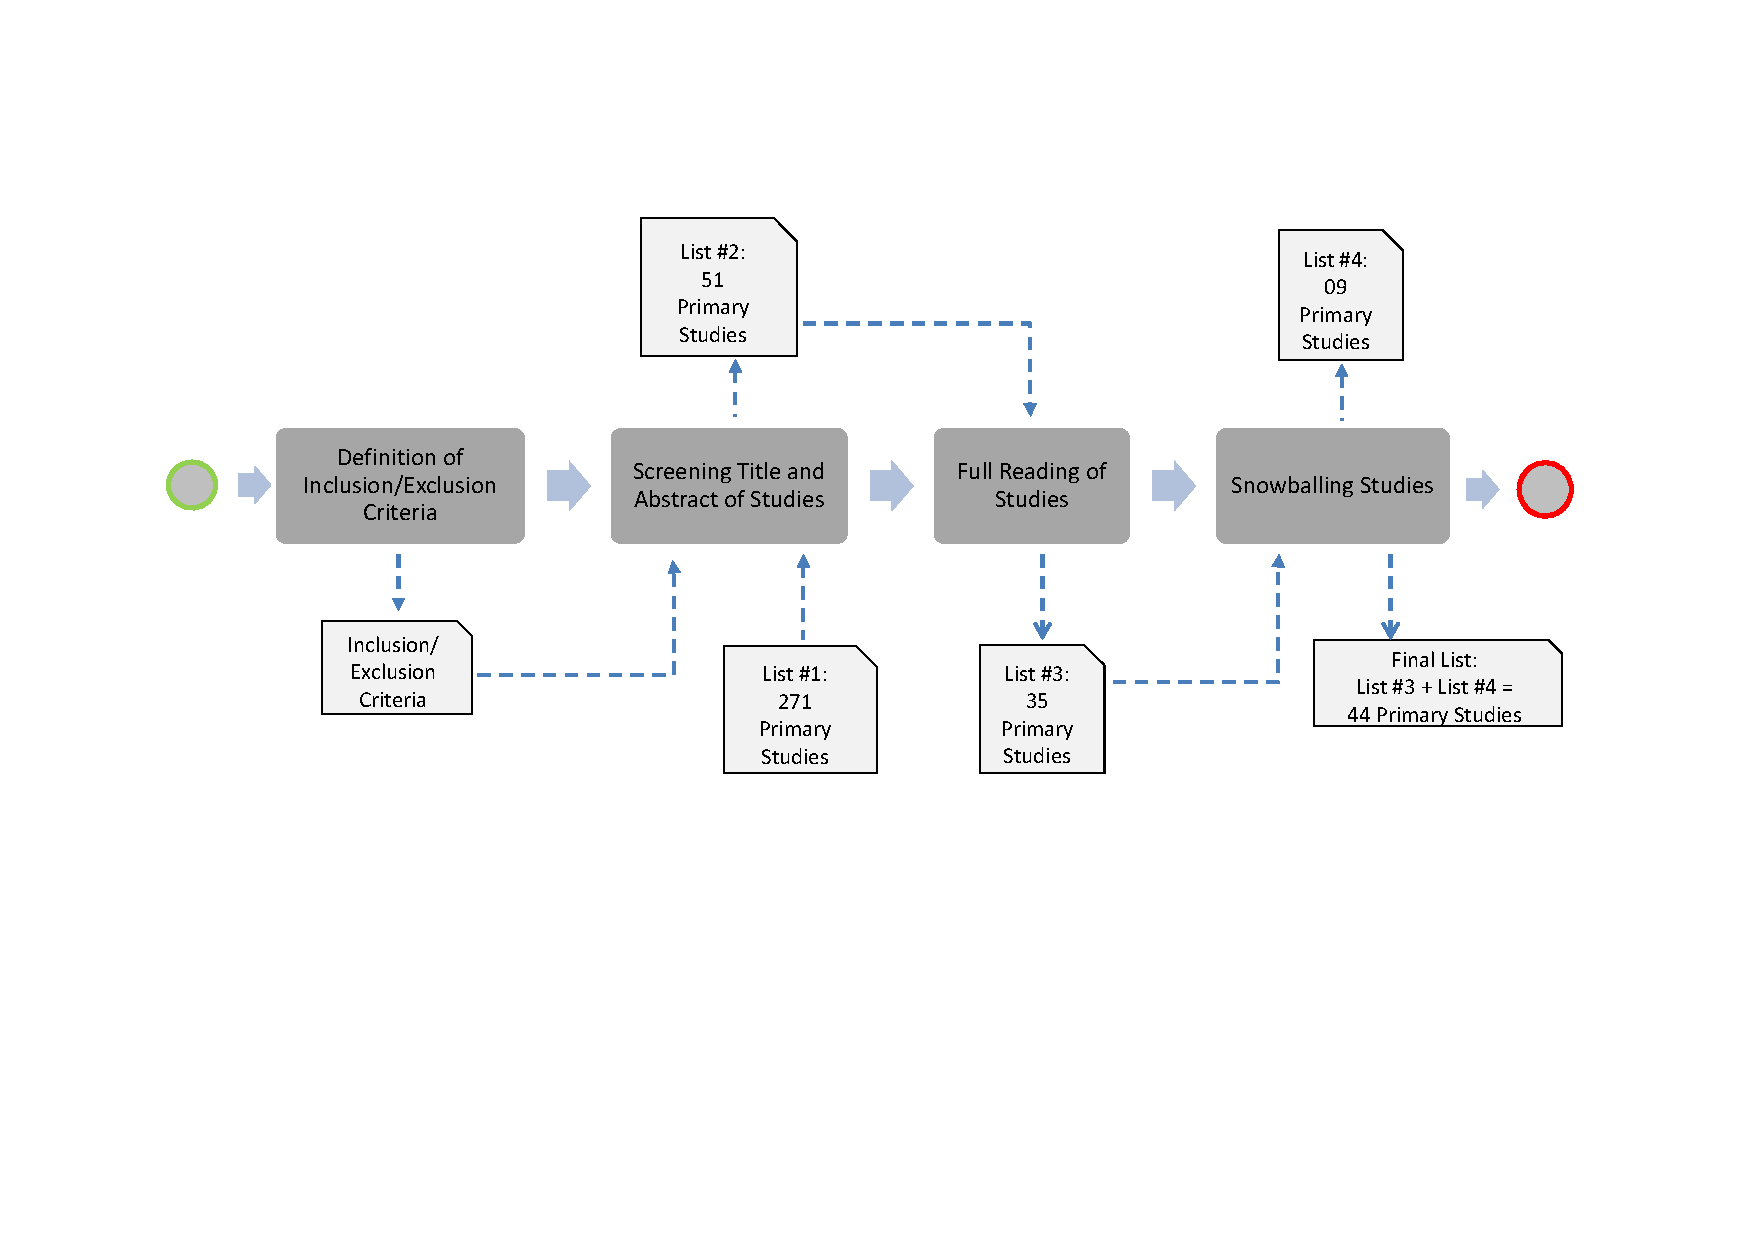
\includegraphics[scale=0.60]{selection_process.pdf}
	\caption{Processo Seletivo MSL}
	\label{fig:selection_process}
\end{figure}

As próximas seções apresentam como realizamos o processo de seleção.

\subsubsection{Definição de Critérios de Inclusão e Exclusão}
\label{sec:criteria}

Para selecionar estudos relevantes e contribuir para responder às questões de pesquisa deste estudo, definimos os seguintes critérios de inclusão e exclusão:

\begin{itemize}
	\item \textbf{Critério de Inclusão:}
	\begin{itemize}
		\item IC.1 - estudos que discutem atividades de TBM realizadas exclusivamente no domínio LPS.
	\end{itemize}
	
	\item \textbf{Critérios de exclusão:}
	\begin{itemize}
		\item EC.1 - estudos não abordam atividades de TBM realizadas exclusivamente no domínio LPS;
		\item EC.2 - estudos com texto incompleto;
		\item EC.3 - estudos em um idioma diferente do inglês para promover a disseminação e reprodutibilidade internacional;
		\item EC.4 - estudos com menos de quatro páginas, pois acreditamos que eles não têm espaço para contribuições relevantes;
		\item EC.5 - estudos duplicados;
		\item EC.6 - estudos indisponíveis, mesmo em contato com os autores.
	\end{itemize}
\end{itemize}

\subsubsection{Títulos de triagem e resumos de estudos}

Depois de definir os critérios de inclusão e exclusão, aplicamos os mesmos aos estudos lendo títulos e resumos de Lista \# 1 (271 estudos). Tal leitura filtrou Lista \# 1 para aceitar 51 estudos (Lista \# 2), onde 40 estudos provêm da busca eletrônica ( \ref{table:buscaauto}, coluna `` Aceito '') e 11 da busca manual ( \ref{table:manualtabela}, coluna `` Aceito '').

\begin{center}
	\begin{tiny}
		\begin{longtable}{l|c|c|c}		
			\caption{Artigos selecionados para leitura completa}
			\label{table:lista51} \\\hline
			
			\textbf{Título} & \textbf{Ano} & \textbf{Local} & \textbf{Tipo Pub.} \\\hline
			\endfirsthead
			
			\multicolumn{4}{c}
			{{\bfseries  \thetable\ Continuação da página anterior}} \\\hline
			\textbf{Título} & \textbf{Ano} & \textbf{Local} & \textbf{Tipo Pub.} \\\hline
			\endhead
			
			
			\begin{tabular}[c]{@{}l@{}}Delta-Oriented Model-Based \\LPS Regression Testing \cite{Lity_et_al2012}\end{tabular} & 2012 & ACM & Evento \\\hline
			
			\begin{tabular}[c]{@{}l@{}}Industrial Evaluation of Pairwise \\LPS Testing with MoSo-PoLiTe \cite{Steffens_et_al2012}\end{tabular} & 2012 & ACM & Evento \\\hline			
			
			\begin{tabular}[c]{@{}l@{}}Model-Based Coverage-Driven \\Test Suite Generation for \\Software Product Lines \cite{cichos2011model}\end{tabular} & 2011 & ACM & Journal \\\hline
			
			\begin{tabular}[c]{@{}l@{}}MoSo-PoLiTe - Tool Support \\for Pairwise and Model-Based \\Software Product Line Testing \cite{oster2011moso}\end{tabular}  & 2011 & ACM & Evento \\\hline
			
			MPLM - MaTeLo Product Line Manager \cite{Samih_et_al2014} & 2014 & ACM & Evento \\\hline
			
			\begin{tabular}[c]{@{}l@{}}On the use of test cases in \\model-based software product line \\development \cite{knapp2014use}\end{tabular} & 2014 & ACM & Evento \\\hline
			
			\begin{tabular}[c]{@{}l@{}}Pairwise Feature-Interaction \\Testing for LPSs:Potentials \\and Limitations \cite{oster2011pairwise}\end{tabular} & 2011 & ACM & Evento \\\hline
			
			\begin{tabular}[c]{@{}l@{}}Deriving Usage Model Variants \\for Model- based Testing:\\An Industrial Case Study \cite{samih2014deriving}\end{tabular} & 2014 & IEEE & Evento \\\hline
			
			\begin{tabular}[c]{@{}l@{}}Model-based Software Product Line \\Testing by Coupling Feature Models \\with Hierarchical Markov Chain Usage Models \cite{gebizli2016model}\end{tabular}  & 2016 & IEEE & Evento \\\hline
			
			\begin{tabular}[c]{@{}l@{}}Model-Based Test Design of Product Lines:\\ Raising Test Design to the Product Line Level\end{tabular} \cite{lackner2014model} & 2014 & IEEE & Journal \\\hline
			
			Requirements-Based Delta-Oriented LPS Testing \cite{dukaczewski2013requirements} & 2013 & IEEE & Evento \\\hline
			
			\begin{tabular}[c]{@{}l@{}}Using Feature Model to Support \\Model-Based Testing of Product Lines:\\An Industrial Case Study\end{tabular} \cite{Wang_et_al2013} & 2013 & IEEE & Journal \\\hline
			
			\begin{tabular}[c]{@{}l@{}}An automated Model-based Testing \\Approach in Software Product Lines \\Using a Variability Language\end{tabular} \cite{Garcia_et_al2010} & 2010 & \begin{tabular}[c]{@{}c@{}}Politécnica \\Arquivo \\digital UPM\end{tabular} & Evento \\\hline
			
			\begin{tabular}[c]{@{}l@{}}Automated Product Line Methodologies \\to Support Model-Based Testing\end{tabular} \cite{wang2013automated} & 2013 & \begin{tabular}[c]{@{}c@{}}CEUR \\Proceedings\end{tabular} & Evento \\\hline
			
			\begin{tabular}[c]{@{}l@{}}Behavioural Model Based Testing \\of Software Product Lines\end{tabular} \cite{devroey2014behavioural} & 2014 & ACM & Evento \\\hline
			
			\begin{tabular}[c]{@{}l@{}}Feature Model-based Software Product\\Line Testing \cite{oster2012feature}\end{tabular} & 2012 & \begin{tabular}[c]{@{}c@{}}TUprints\\Darmstadt \\publication \\service\end{tabular} & Journal \\\hline
			
			\begin{tabular}[c]{@{}l@{}}Model-based pairwise testing \\for feature interaction coverage \\in software product line engineering\end{tabular} \cite{lochau2012model} & 2011 & Springer & Journal \\\hline
			
			\begin{tabular}[c]{@{}l@{}}Model-based Test Generation \\for Software Product Line\end{tabular} \cite{cai2013model} & 2013 & IEEE & Evento \\\hline
			
			Model-Based Testing for Software Product Lines \cite{Olimpiew2008} & 2008 & Springer & Evento \\\hline
			
			\begin{tabular}[c]{@{}l@{}}PLETS - A Product Line \\of Model- Based Testing Tools\end{tabular} \cite{rodrigues2013plets} & 2013 & PUC-RS & Evento \\\hline
			
			\begin{tabular}[c]{@{}l@{}}Top-Down and Bottom-Up \\Approach for Model-Based \\Testing of Product Lines\end{tabular} \cite{weissleder2013top} & 2013 & EPTCS & Evento \\\hline
			
			\begin{tabular}[c]{@{}l@{}}A Product Line Modeling and \\Configuration Methodology to \\Support Model-Based Testing:\\An Industrial Case Study\end{tabular} \cite{ali2012product} & 2012 & Springer & Journal \\\hline
			
			\begin{tabular}[c]{@{}l@{}}Coverage Criteria for Behavioural \\Testing of Software Product Lines\end{tabular} \cite{devroey2014coverage} & 2014 & Springer & Evento \\\hline
			
			\begin{tabular}[c]{@{}l@{}}A Model Based Testing Approach \\for Model-Driven Development \\and Software Product Lines\end{tabular} \cite{Lamancha_et_al2010} & 2010 & Springer & Evento \\\hline
			
			\begin{tabular}[c]{@{}l@{}}A Vision for Behavioural Model-Driven \\Validation of Software Product Lines\end{tabular} \cite{devroey2012vision} & 2012 & Springer & Evento \\\hline
			
			\begin{tabular}[c]{@{}l@{}}Abstract Test Case Generation for\\Behavioural Testing of Software Product Lines\end{tabular} \cite{devroey2014abstract} & 2014 & ACM & Evento \\\hline
			
			\begin{tabular}[c]{@{}l@{}}Applying Incremental Model Slicing \\to Product-Line Regression Testing\end{tabular} \cite{lity2016applying} & 2016 & Springer & Journal \\\hline
			
			\begin{tabular}[c]{@{}l@{}}Automated Testing of Software-as-a-Service \\Configurations using a Variability Language\end{tabular} \cite{patel2015automated} & 2015 & ACM & Evento \\\hline
			
			Delta-Oriented FSM-Based Testing \cite{varshosaz2015delta} & 2015 & Springer & Evento \\\hline
			
			\begin{tabular}[c]{@{}l@{}}Incremental Model-Based Testing \\of Delta-oriented Software Product Lines\end{tabular} \cite{lochau2012incremental} & 2012 & Springer & Journal \\\hline
			
			Model Based Testing in Software Product Lines \cite{Reales_et_al2011} & 2011 & Springer & Evento \\\hline
			
			Model-Based Testing \cite{Lochau:2014} & 2014 & Springer & Evento \\\hline
			
			\begin{tabular}[c]{@{}l@{}}Parameterized Preorder Relations for Model-Based\\Testing of Software Product Lines\end{tabular} \cite{lochau2012parameterized} & 2012 & Springer & Evento \\\hline
			
			\begin{tabular}[c]{@{}l@{}}Poster:VIBeS, Transition \\System Mutation Made Easy\end{tabular} \cite{devroey2015vibes} & 2015 & IEEE & Evento \\\hline
			
			Spinal Test Suites for Software Product Lines \cite{beohar2014spinal} & 2014 & EPTCS & Evento \\\hline
			
			\begin{tabular}[c]{@{}l@{}}Automated model-based testing \\using the UML testing profile and QVT\end{tabular} \cite{Lamancha_et_al2009} & 2009 & ACM & Evento \\\hline
			
			\begin{tabular}[c]{@{}l@{}}Relating Variability Modeling and \\Model-Based Testing for \\Software Product Lines Testing\end{tabular} \cite{samih2012relating} & 2012 & ICTSS & Evento \\\hline
			
			\begin{tabular}[c]{@{}l@{}}An Evaluation of Model-Based Testing \\in Embedded Applications\end{tabular} \cite{weissleder2014evaluation} & 2014 & IEEE & Evento \\\hline
			
			\begin{tabular}[c]{@{}l@{}}Assessing Software Product Line Testing \\Via Model-Based Mutation \\An Application to Similarity Testing\end{tabular} \cite{henard2013assessing} & 2013 & IEEE & Evento \\\hline
			
			\begin{tabular}[c]{@{}l@{}}Automated and Scalable T-wise \\Test Case Generation Strategies \\for Software Product Lines\end{tabular} \cite{perrouin2010automated} &  2010 & IEEE & Evento \\\hline
			
			\begin{tabular}[c]{@{}l@{}}Model-based Testing of System Requirements \\using UML Use Case Models\end{tabular} \cite{hasling2008model}  & 2008 & IEEE & Evento \\\hline
			
			\begin{tabular}[c]{@{}l@{}}Successive refinement of models \\for model-based testing to increase system \\test effectiveness\end{tabular} \cite{gebizli2016successive} & 2016 & IEEE & Evento \\\hline
			
			\begin{tabular}[c]{@{}l@{}}A Software Product Line \\for Model-Based Testing Tools\end{tabular} \cite{rodrigues2012software}  & 2012 & PUC-RS & Evento \\\hline
			
			\begin{tabular}[c]{@{}l@{}}Reusing State Machines for Automatic Test \\Generation in Product Lines\end{tabular} \cite{weissleder2008reusing}  & 2008 & MoTip & Evento \\\hline
			
			\begin{tabular}[c]{@{}l@{}}A Nãovel Markov Boundary Based Feature \\Subset Selection Algorithm\end{tabular} \cite{de2010novel}  & 2010 & Elsevier & Journal \\\hline
			
			\begin{tabular}[c]{@{}l@{}}A Nãovel Model-Based Testing Approach for \\Software Product Lines\end{tabular} \cite{damiani2017novel}  & 2016 & Springer & Evento \\\hline
			
			\begin{tabular}[c]{@{}l@{}}Abstract Test Case Generation for Behavioural\\Testing of Software Product Lines\end{tabular} \cite{devroey2014abstract}  & 2014 & ACM & Evento \\\hline				
			
			\begin{tabular}[c]{@{}l@{}}An Overview on Test Generation from \\Functional Requirements \end{tabular} \cite{escalona2011overview}  &  2011 & Elsevier & Journal \\\hline				
			
			\begin{tabular}[c]{@{}l@{}}Basic Behavioral Models for Software\\Product Lines:Expressiveness and Testing \\Pre-Orders \end{tabular} \cite{beohar2016basic}  & 2016 & Elsevier & Journal \\\hline
			
			\begin{tabular}[c]{@{}l@{}}Bottom-up reuse for multi-level testing \end{tabular} \cite{perez2010bottom}  & 2010 & Elsevier & Journal \\\hline
			
			\begin{tabular}[c]{@{}l@{}}Colored Model Based Testing for \\Software Product Lines \end{tabular} \cite{farrag2010colored}  & 2010 & semanticscholar & Gray Literature \\\hline
			
			\begin{tabular}[c]{@{}l@{}}IncLing:Efficient Product-Line Testing Using\\Incremental Pairwise Sampling \end{tabular} \cite{al2016incling}  & 2016 & ACM & Evento \\\hline
			
			\begin{tabular}[c]{@{}l@{}}Input-output conformance testing based \\on featured transition systems \end{tabular} \cite{beohar2014input}  & 2014 & ACM & Evento \\\hline
			
			\begin{tabular}[c]{@{}l@{}}Model-based testing of automotive systems \end{tabular} \cite{bringmann2008model}  & 2008 & IEEE & Evento \\\hline
			
			\begin{tabular}[c]{@{}l@{}}Model-based system testing of \\software product families \end{tabular} \cite{reuys2005model}  & 2005 & Springer & Evento \\\hline
			
			\begin{tabular}[c]{@{}l@{}}Model-based testing for applications \\derived from software product lines \end{tabular} \cite{olimpiew2005model}  & 2005 & ACM & Evento \\\hline
			
			\begin{tabular}[c]{@{}l@{}}Reducing the Concretization Effort in\\FSM-Based Testing of Software Product Lines \end{tabular} \cite{fragal2017reducing}  & 2016 & IEEE & Evento \\\hline
			
			\begin{tabular}[c]{@{}l@{}}Refinement-based testing of \\delta-oriented product lines \end{tabular} \cite{damiani2013refinement}  & 2013 & ACM & Evento \\\hline
			
			\begin{tabular}[c]{@{}l@{}}Risk-based integration testing of \\software product lines \end{tabular} \cite{lachmann2017risk}  & 2016 & ACM & Evento \\\hline
			
			\begin{tabular}[c]{@{}l@{}}Uncertainty-wise evolution of \\test ready models \end{tabular} \cite{zhang2017uncertainty}  & 2016 & Elsevier & Journal \\\hline
		\end{longtable}
	\end{tiny}
\end{center}

\subsubsection{Leitura Completa de Estudos}

Dada Lista \# 2, lemos cada um dos 51 estudos. Rejeitamos 16 deles (veja \ref{table:lista16}) com base nos critérios de exclusão da Seção \ref{sec:criteria}, fornecendo assim Lista \# 3 com 35 estudos.

% \usepackage{array}
% \usepackage{longtable}

\begin{small}
	

\begin{longtable}{>{\hspace{0pt}}p{0.452\linewidth}|>{\centering\hspace{0pt}}p{0.059\linewidth}|>{\centering\hspace{0pt}}p{0.059\linewidth}|>{\centering\hspace{0pt}}p{0.059\linewidth}|>{\centering\hspace{0pt}}p{0.059\linewidth}|>{\centering\hspace{0pt}}p{0.059\linewidth}|>{\centering\arraybackslash\hspace{0pt}}p{0.059\linewidth}}
\caption{Estudos removidos de acordo com os critérios de exclusão}
\label{table:lista16}\\ 
	\hline
	\textbf{Título}  & \textbf{EC.1}  & \textbf{EC.2}  & \textbf{EC.3}  & \textbf{EC.4}  & \textbf{EC.5}  & \textbf{EC.6}  \endfirsthead 
	\hline
	A Novel Markov Boundary Based Feature Subset Selection Algorithm  & X & - & - & - & - & - \\ 
	\hline
	A Nãovel Model-Based Testing Approach for Software Product Lines  & - & - & - & - & X & - \\ 
	\hline
	Abstract Test Case Generation for Behavioural Testing of Software Product Lines  & X & - & - & - & - & - \\ 
	\hline
	An Overview on Test Generation from Functional Requirements  & X & - & - & - & - & - \\ 
	\hline
	Basic Behavioral Models for Software Product Lines:Expressiveness and Testing Pre-Orders  & - & - & - & X & - & - \\ 
	\hline
	Bottom-up reuse for multi-level testing & X & - & - & - & - & - \\ 
	\hline
	Colored Model Based Testing for Software Product Lines  & X & - & - & - & X & - \\ 
	\hline
	IncLing:Efficient Product-Line Testing Using Incremental Pairwise Sampling  & X & - & - & - & - & - \\ 
	\hline
	Input-output conformance testing based on featured transition systems  & X & - & - & - & - & - \\ 
	\hline
	Model-based testing of automotive systems & - & - & - & X & - & - \\ 
	\hline
	Model-based system testing of software product families  & - & - & - & - & X & - \\ 
	\hline
	Model-based testing for applications derived from software product lines  & - & - & - & - & X & - \\ 
	\hline
	Reducing the Concretization Effort in FSM-Based Testing of Software Product Lines  & X & - & - & - & - & - \\ 
	\hline
	Refinement-based testing of delta-oriented product lines  & X & - & - & - & - & - \\ 
	\hline
	Risk-based integration testing of software product lines  & X & - & - & - & - & - \\ 
	\hline
	Uncertainty-wise evolution of test ready models  & X & - & - & - & - & - \\
	\hline
\end{longtable}
\end{small}


\subsubsection{Estudos derivados do Snowballing}

Realizamos bolas de neve invertidas em Lista \# 3, onde avaliamos as referências dos estudos. Dez estudos retornaram de bola de neve, e os critérios de inclusão e exclusão foram aplicados a eles. Portanto, um deles foi duplicado conforme apresentado em \ref{table:snow}. Os nove estudos restantes compuseram Lista \# 4.

% \usepackage{array}
% \usepackage{pdflscape}
% \usepackage{longtable}


	
\begin{small}


\begin{landscape}
	\begin{longtable}
		{>{\centering\hspace{0pt}}p{0.025\linewidth}|>{\hspace{0pt}}p{0.400\linewidth}|>{\centering\hspace{0pt}}p{0.025\linewidth}|>{\hspace{0pt}}p{0.435\linewidth}|>{\centering\arraybackslash\hspace{0pt}}p{0.080\linewidth}}
		\caption*{Estudos do Snowballing\label{table:snow}}\\ 
		\hline\hline
		\textbf{ID}  & \multicolumn{1}{>{\centering\hspace{0pt}}p{0.381\linewidth}|}{\textbf{Fonte do estudo} } & \textbf{ID}  & \multicolumn{1}{>{\centering\hspace{0pt}}p{0.415\linewidth}|}{\textbf{Estudo do Snowballing} } & \textbf{Estatus}  \endfirsthead 
		\hline\hline
		S24 & A Model Based Testing Approach for Model-Driven Development and Software Product Lines  & S36 & Automated model-based testing using the UML testing profile and QVT  & Aceito \\ 
		\hline
		S8 & Deriving Usage Model Variants for Model-based Testing:An Industrial Case Study  & S37 & Relating Variability Modeling and Model-Based Testing for Software Product Lines Testing  & Aceito \\ 
		\hline
		S10 & Model-Based Test Design of Product Lines:Raising Test Design to the Product Line Level  & S38 & An Evaluation of Model-Based Testing in Embedded Applications  & Aceito \\ 
		\hline
		S10 & Model-Based Test Design of Product Lines:Raising Test Design to the Product Line Level  & S39 & Assessing Software Product Line Testing Via Model-Based Mutation An Application to Similarity Testing  & Aceito \\ 
		\hline
		S5 & MPLM-MaTeLo Product Line Manager & S40 & Automated and Scalable T-wise Test Case Generation Strategies for Software Product Lines  & Aceito \\ 
		\hline
		S20 & PLETS - a Product Line of Model-Based Testing Tools  & S41 & Model based testing of system requirements using UML use case models  & Aceito \\ 
		\hline
		S9 & Model-based Software Product Line Testing by Coupling Feature Models with Hierarchical Markov Chain Usage Models  & S42 & Successive refinement of models for model-based testing to increase system test effectiveness  & Aceito \\ 
		\hline
		S20 & PLETS - a Product Line of Model-Based Testing Tools  & S43 & A Software Product Line for Model-Based Testing Tools  & Aceito \\ 
		\hline
		S21 & Top-Down and Bottom-Up Approach for Model-Based Testing of Product Lines  & S44 & Reusing State Machines for Automatic Test Generation in Product Lines  & Aceito \\ 
		\hline
		S5 & MPLM-MaTeLo Product Line Manager & – & An approach to derive usage models variants for model-based  & Duplicado \\
		\hline\hline
	\end{longtable}
\end{landscape}
\end{small}


A \ref{table:listaextra} apresenta o conjunto final de estudos selecionados para este MSL, composto por 44 estudos (Lista Final), dos quais:os primeiros 35 são de pesquisas eletrônicas e manuais e os restantes nove são do \textit{Snowballing}.

%\textcolor{red}{COLOCAR O \ CITE DE CADA TRABALHO ANTES DO \FIM{TABULAR} COMO NOS TRABALHOS DE S1 A 29 ...}

\begin{center}
	\begin{tiny}
		\begin{longtable}{c|l|c|c|c}		
			\caption{Lista final de estudos}
			\label{table:listaextra} \\\hline
			
			\textbf{ID} & \multicolumn{1}{c|}{\textbf{Título}} & \textbf{Ano} & \textbf{Local} & \textbf{Tipo de Pub.} \\\hline
			\endfirsthead
			
			\multicolumn{5}{c}
			{{\bfseries  \thetable\ Continuação da página anterior}} \\\hline
			\textbf{ID} & \multicolumn{1}{c|}{\textbf{Título}} & \textbf{Ano} & \textbf{Local} & \textbf{Tipo de Pub.} \\\hline
			\endhead
			
			
			S1 & \begin{tabular}[c]{@{}l@{}}Delta-Oriented Model-Based \\LPS Regression Testing \cite{Lity_et_al2012}\end{tabular} & 2012 & ACM & Evento \\\hline
			
			S2 & \begin{tabular}[c]{@{}l@{}}Industrial Evaluation of Pairwise \\LPS Testing with MoSo-PoLiTe \cite{Steffens_et_al2012}\end{tabular} & 2012 & ACM & Evento \\\hline
			S3 & \begin{tabular}[c]{@{}l@{}}Model-Based Coverage-Driven \\Test Suíte Generation for \\Software Product Lines \cite{cichos2011model}\end{tabular} & 2011 & ACM & Journal \\\hline
			S4 & \begin{tabular}[c]{@{}l@{}}MoSo-PoLiTe - Tool Support \\for Pairwise and Model-Based \\Software Product Line Testing \cite{oster2011moso}\end{tabular}  & 2011 & ACM & Evento \\\hline
			S5 & MPLM - MaTeLo Product Line Manager \cite{samih2014mplm} & 2014 & ACM & Evento \\\hline
			S6 & \begin{tabular}[c]{@{}l@{}}On the use of test cases in \\model-based software product line \\development \cite{knapp2014use}\end{tabular} & 2014 & ACM & Evento \\\hline
			S7 & \begin{tabular}[c]{@{}l@{}}Pairwise Feature-Interaction \\Testing for LPSs:Potentials \\and Limitations \cite{oster2011pairwise}\end{tabular} & 2011 & ACM & Evento \\\hline
			S8 & \begin{tabular}[c]{@{}l@{}}Deriving Usage Model Variants \\for Model- based Testing:\\An Industrial Case Study \cite{samih2014deriving}\end{tabular} & 2014 & IEEE & Evento \\\hline
			S9 & \begin{tabular}[c]{@{}l@{}}Model-based Software Product Line \\Testing by Coupling Feature Models \\with Hierarchical Markov Chain Usage Models \cite{gebizli2016model}\end{tabular}  & 2016 & IEEE & Evento \\\hline
			S10 & \begin{tabular}[c]{@{}l@{}}Model-Based Test Design of Product Lines:\\ Raising Test Design to the Product Line Level \cite{lackner2014model}\end{tabular} & 2014 & IEEE & Journal \\\hline
			
			S11 & Requirements-Based Delta-Oriented LPS Testing \cite{dukaczewski2013requirements} & 2013 & IEEE & Evento \\\hline
			
			
			S12 & \begin{tabular}[c]{@{}l@{}}Using Feature Model to Support \\Model-Based Testing of Product Lines:\\An Industrial Case Study \cite{Wang_et_al2013}\end{tabular}  & 2013 & IEEE & Journal \\\hline
			S13 & \begin{tabular}[c]{@{}l@{}}An automated Model-based Testing \\Approach in Software Product Lines \\Using a Variability Language \cite{Garcia_et_al2010}\end{tabular} & 2010 & \begin{tabular}[c]{@{}c@{}}Politécnica \\Arquivo \\digital UPM\end{tabular} & Evento \\\hline
			S14 & \begin{tabular}[c]{@{}l@{}}Automated Product Line Methodologies \\to Support Model-Based Testing \cite{wang2013automated} \end{tabular} & 2013 & \begin{tabular}[c]{@{}c@{}}CEUR \\Proceedings\end{tabular} & Evento \\\hline
			S15 & \begin{tabular}[c]{@{}l@{}}Behavioural Model Based Testing \\of Software Product Lines\end{tabular} \cite{devroey2014behavioural} & 2014 & ACM & Evento \\\hline
			S16 & Feature Model-based Software Product Line Testing \cite{oster2012feature} & 2012 & \begin{tabular}[c]{@{}c@{}}TUprints\\Darmstadt \\publication \\service\end{tabular} & Journal \\\hline
			S17 & \begin{tabular}[c]{@{}l@{}}Model-based pairwise testing \\for feature interaction coverage \\in software product line engineering\end{tabular} \cite{lochau2012model} & 2011 & Springer & Journal \\\hline
			S18 & \begin{tabular}[c]{@{}l@{}}Model-based Test Generation \\for Software Product Line\end{tabular} \cite{cai2013model} & 2013 & IEEE & Evento \\\hline
			S19 & Model-Based Testing for Software Product Lines \cite{Olimpiew2008} & 2008 & Springer & Evento \\\hline
			S20 & \begin{tabular}[c]{@{}l@{}}PLETS - A Product Line \\of Model- Based Testing Tools\end{tabular} \cite{rodrigues2013plets} & 2013 & PUC-RS & Evento \\\hline
			S21 & \begin{tabular}[c]{@{}l@{}}Top-Down and Bottom-Up \\Approach for Model-Based \\Testing of Product Lines\end{tabular} \cite{weissleder2013top} & 2013 & EPTCS & Evento \\\hline
			S22 & \begin{tabular}[c]{@{}l@{}}A Product Line Modeling and \\Configuration Methodology to \\Support Model-Based Testing:\\An Industrial Case Study\end{tabular} \cite{ali2012product} & 2012 & Springer & Journal \\\hline
			S23 & \begin{tabular}[c]{@{}l@{}}Coverage Criteria for Behavioural \\Testing of Software Product Lines\end{tabular} \cite{devroey2014coverage} & 2014 & Springer & Evento \\\hline
			S24 & \begin{tabular}[c]{@{}l@{}}A Model Based Testing Approach \\for Model-Driven Development \\and Software Product Lines\end{tabular} \cite{Lamancha_et_al2010} & 2010 & Springer & Evento \\\hline
			S25 & \begin{tabular}[c]{@{}l@{}}A Vision for Behavioural Model-Driven \\Validation of Software Product Lines\end{tabular} \cite{devroey2012vision} & 2012 & Springer & Evento \\\hline
			S26 & \begin{tabular}[c]{@{}l@{}}Abstract Test Case Generation for\\Behavioural Testing of Software Product Lines\end{tabular} \cite{devroey2014abstract} & 2014 & ACM & Evento \\\hline
			S27 & \begin{tabular}[c]{@{}l@{}}Applying Incremental Model Slicing \\to Product-Line Regression Testing\end{tabular} \cite{lity2016applying} & 2016 & Springer & Journal \\\hline
			S28 & \begin{tabular}[c]{@{}l@{}}Automated Testing of Software-as-a-Service \\Configurations using a Variability Language\end{tabular} \cite{patel2015automated} & 2015 & ACM & Evento \\\hline
			S29 & Delta-Oriented FSM-Based Testing \cite{varshosaz2015delta} & 2015 & Springer & Evento \\\hline
			S30 & \begin{tabular}[c]{@{}l@{}}Incremental Model-Based Testing \\of Delta-oriented Software Product Lines\end{tabular} \cite{lochau2012incremental} & 2012 & Springer & Journal \\\hline
			S31 & Model Based Testing in Software Product Lines \cite{Reales_et_al2011} & 2011 & Springer & Evento \\\hline
			S32 & Model-Based Testing \cite{Lochau:2014} & 2014 & Springer & Evento \\\hline
			S33 & \begin{tabular}[c]{@{}l@{}}Parameterized Preorder Relations \\for Model-Based Testing of Software Product Lines\end{tabular} \cite{lochau2012parameterized} & 2012 & Springer & Evento \\\hline
			S34 & \begin{tabular}[c]{@{}l@{}}Poster:VIBeS, Transition \\System Mutation Made Easy\end{tabular} \cite{devroey2015vibes} & 2015 & IEEE & Evento \\\hline
			S35 & Spinal Test Suites for Software Product Lines \cite{beohar2014spinal} & 2014 & EPTCS & Evento \\\hline
			
			
			S36 & \begin{tabular}[c]{@{}l@{}}Automated model-based testing \\using the UML testing profile and QVT\end{tabular} \cite{Lamancha_et_al2009} & 2009 & ACM & Evento \\\hline
			S37 & \begin{tabular}[c]{@{}l@{}}Relating Variability Modeling and \\Model-Based Testing for \\Software Product Lines Testing\end{tabular} \cite{samih2012relating} & 2012 & ICTSS & Evento \\\hline
			S38 & \begin{tabular}[c]{@{}l@{}}An Evaluation of Model-Based Testing \\in Embedded Applications\end{tabular} \cite{weissleder2014evaluation} & 2014 & IEEE & Evento \\\hline
			S39 & \begin{tabular}[c]{@{}l@{}}Assessing Software Product Line Testing \\Via Model-Based Mutation \\An Application to Similarity Testing\end{tabular} \cite{henard2013assessing} & 2013 & IEEE & Evento \\\hline
			S40 & \begin{tabular}[c]{@{}l@{}}Automated and Scalable T-wise \\Test Case Generation Strategies \\for Software Product Lines\end{tabular} \cite{perrouin2010automated} & 2010 & IEEE & Evento \\\hline
			S41 & \begin{tabular}[c]{@{}l@{}}Model-based Testing of System Requirements \\using UML Use Case Models\end{tabular} \cite{hasling2008model}  & 2008 & IEEE & Evento \\\hline
			S42 & \begin{tabular}[c]{@{}l@{}}Successive refinement of models \\for model-based testing to increase system \\test effectiveness\end{tabular} \cite{gebizli2016successive} & 2016 & IEEE & Evento \\\hline
			S43 & \begin{tabular}[c]{@{}l@{}}A Software Product Line \\for Model-Based Testing Tools\end{tabular} \cite{rodrigues2012software}  & 2012 & PUC-RS & Evento \\\hline
			S44 & \begin{tabular}[c]{@{}l@{}}Reusing State Machines for Automatic Test \\Generation in Product Lines\end{tabular} \cite{weissleder2008reusing}  & 2008 & MoTip & Evento \\\hline				
		\end{longtable}
	\end{tiny}
\end{center}

\subsection{Processo de Extração}
\label{sec:extraction_process}

A \ref{fig:extraction_process} mostra o processo de extração do MSL.

\begin{figure}[!h]
	\centering
	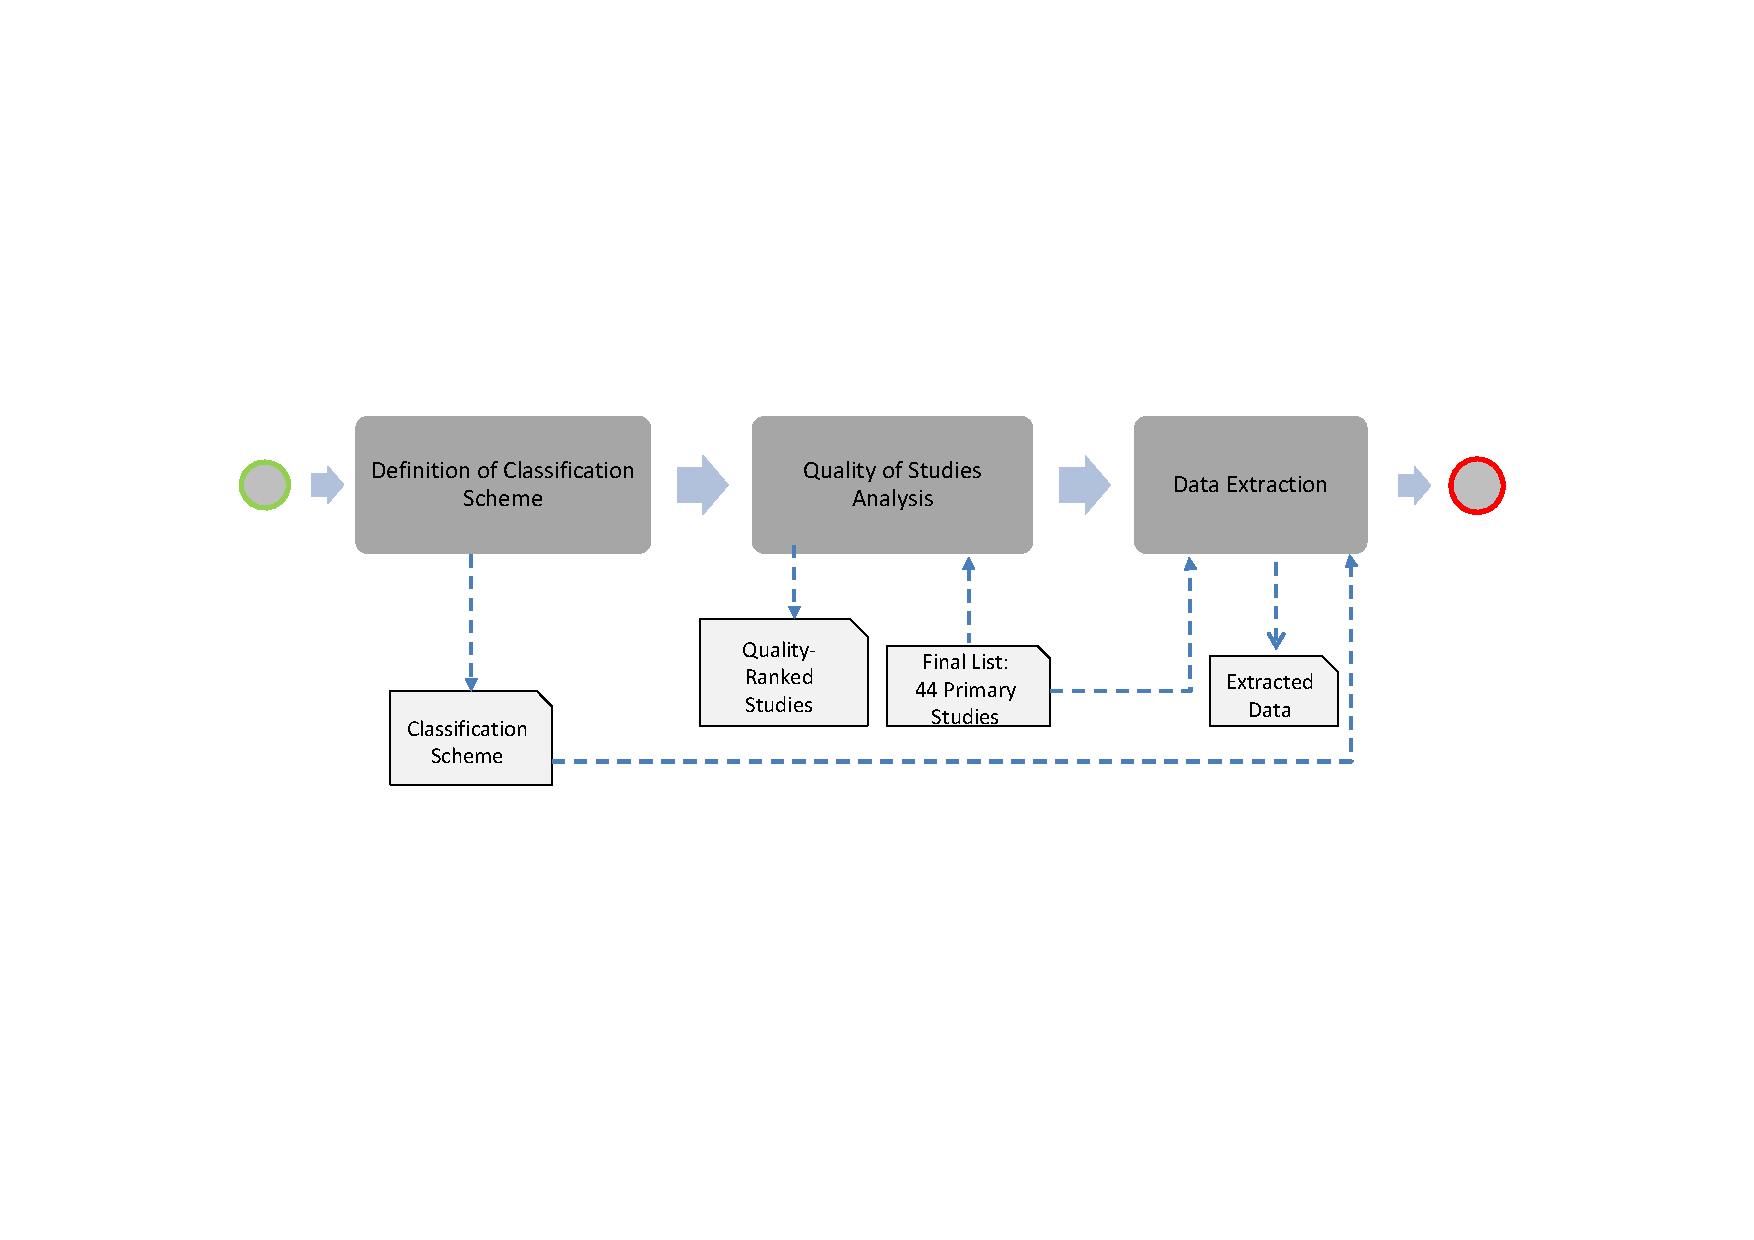
\includegraphics[scale=0.60]{extraction_process.pdf}
	\caption{Processo de extração de MSL}
	\label{fig:extraction_process}
\end{figure}

\subsubsection{Definição do Esquema de Classificação}

\subsubsection{Análise de Qualidade de Estudos}
\label{sec:quality_analysis}

Para avaliação da qualidade dos estudos, definimos um questionário e aplicamos em cada estudo. Portanto, elaboramos as três perguntas a seguir:

\begin{itemize}
	\item O par de estudos é revisado?
	\item O objetivo do estudo é claro?
	\item A proposta do estudo foi avaliada / validada?
\end{itemize}

Para cada questão, havia três alternativas, nas quais apenas uma delas poderia ser escolhida:`` Não '', `` Sim '' e `` Parcialmente ''. Estudos com `` Não '' para quaisquer questões são automaticamente descartados. Nós cuidadosamente lemos novamente os estudos com "Parcialidade" como uma resposta para qualquer pergunta.

Adotamos este procedimento, assim como a aplicação dos critérios de inclusão e exclusão para garantir contribuições mínimas dos estudos selecionados para o processo de extração.

Realizamos a extração de dados para coletar informações necessárias para responder às questões de pesquisa, bem como analisar os estudos dos critérios de seleção. Portanto, definimos os seguintes critérios de qualidade (QC) para garantir a qualidade mínima dos estudos:

\begin{itemize}
	\item QC.1 - O estudo descreve claramente o propósito da pesquisa?
	\item QC.2 - O campo de ação é compatível com a área de pesquisa?
	\item QC.3 - Como o estudo é avaliado?
	\item QC.4 - Houve uma coleta de dados apropriada?
	\item QC.5 - Houve uma análise de dados apropriada?
	\item QC.6 - O estudo apresenta resultados consistentes com seus objetivos?
	\item QC.7 - Os resultados contribuem para o processo realizado para a pesquisa?
\end{itemize}



\subsubsection{Extração de dados}

Os próximos itens apresentam a lista de dados que definimos como extraídos de cada estudo primário:

\begin{itemize}
	\item Dados bibliométricos:Título, Autor(es), Ano de Publicação, Fonte de Publicação, Tipo de Publicação, Tipo de Documento;
	\item Domínio da Solução;
	\item Inclui variabilidade ?;
	\item \textit{Feature Interaction}?;
	\item Método de Execução;
	\item Item de teste usado;
	\item Nível de teste aplicado;
	\item Abordagem de Teste Usada;
	\item Nível de cobertura;
	\item Trate a rastreabilidade ?;
	\item Finalidade do TBM;
	\item Teste de Requisito Não-Funcional é Suportado ?;
	\item Artefato de Origem;
	\item Artefato Intermediário;
	\item Uso de Ferramentas;
	\item Tempo de Ligação;
	\item Atividades do TBM avaliadas;
	\item Resultados da pesquisa;
	\item Método de Coleta de Evidências;
	\item Local de validação;
	\item Tipo de contribuição.
	
\end{itemize}

\subsection{Processo de Análise}
\label{sec:analysis_process}

A \ref{fig:analysis_process} mostra o processo de análise do MSL.

\begin{figure} [!h]
	\centering
	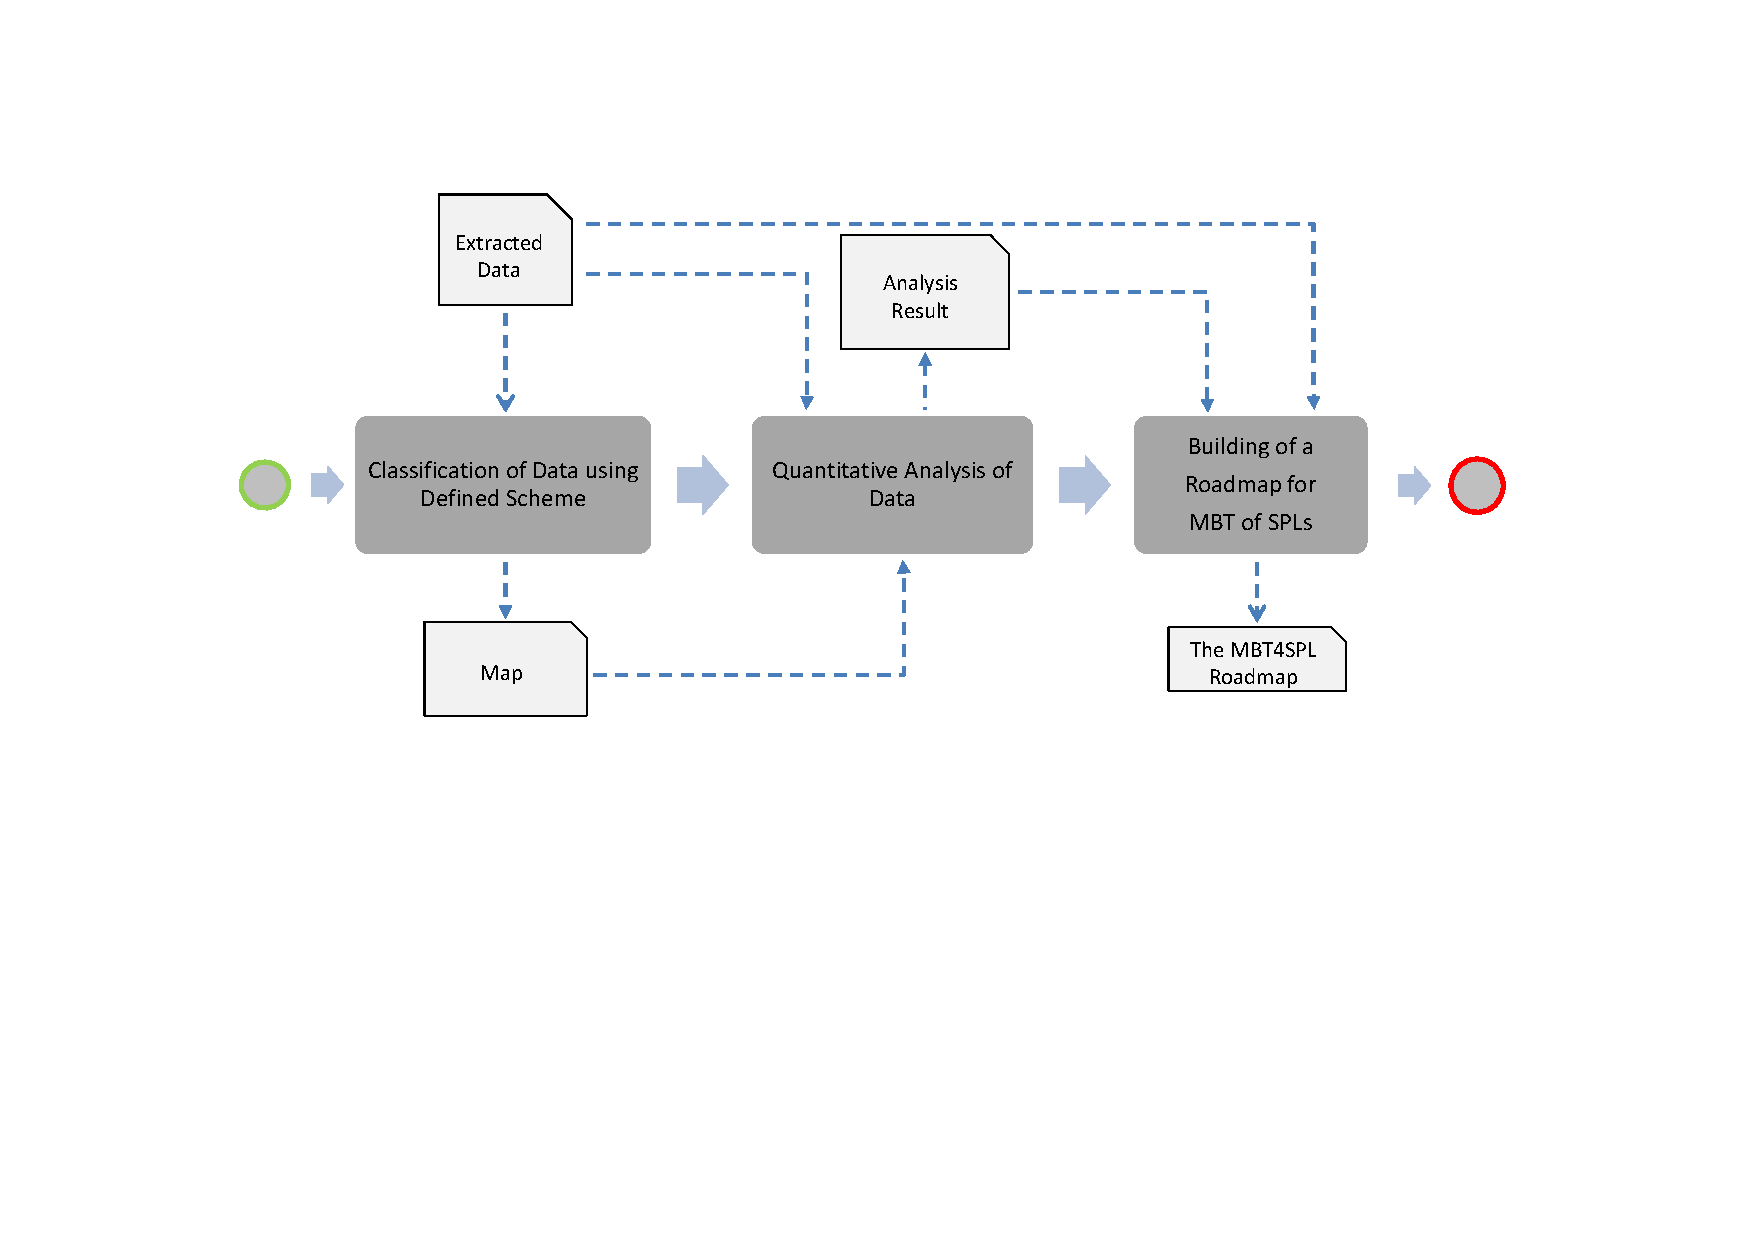
\includegraphics[scale=0.60]{analysis_process.pdf}
	\caption{Processo de Análise MSL}
	\label{fig:analysis_process}
\end{figure}

Classificação de dados usando o esquema definido

Análise Quantitativa de Dados

Criação de um roteiro para TBM de LPSs

\section{Resultados}
\label{sec:secmsl_results}

\subsection{Caracterização dos Estudos}

\subsubsection{Estudos por ano}

É importante entender como o tema de pesquisa do TBM aplicado ao LPS se comportou ao longo dos últimos anos. Portanto, \ref{table:listaano} apresenta o número de estudos por ano e a \ref{fig:qtdano} mostra a distribuição desses estudos ao longo dos anos.

\begin{table}[!h]
	\centering
	\tiny
	\caption{Número de estudos por ano}
	\label{table:listaano}
	
	\begin{tabular}{l|c|c|c|c|c|c|c|c|c|c} \hline 
		
		\textbf{Tipo de local} & \textbf{2008} & \textbf{2009} & \textbf{2010} & \textbf{2011} & \textbf{2012} & \textbf{2013} & \textbf{2014} & \textbf{2015} & \textbf{2016} & \textbf{Count}\\\hline \hline
		
		
		Conferência &  1 & 1 & 1 & 2 & - & 3 & 6 & 3 & 2 & 19 \\\hline
		
		Workshop &  2 & 1 & 1 & 1 & 4 & 3 & 1 & - & - & 13 \\\hline
		
		Journal &  - & - & - & 2 & 3 & 1 & 1 & - & 1 & 8 \\\hline
		
		Simpósio & - & - & - & - & 2 & - & 2 & - & - & 4 \\\hline
		
		Total &  3 & 2 & 2 & 5 & 9 & 7 & 10 & 3 & 3 & 44 \\\hline
		
		
		
	\end{tabular}
\end{table}

\begin{figure}[!h]
	\centering
	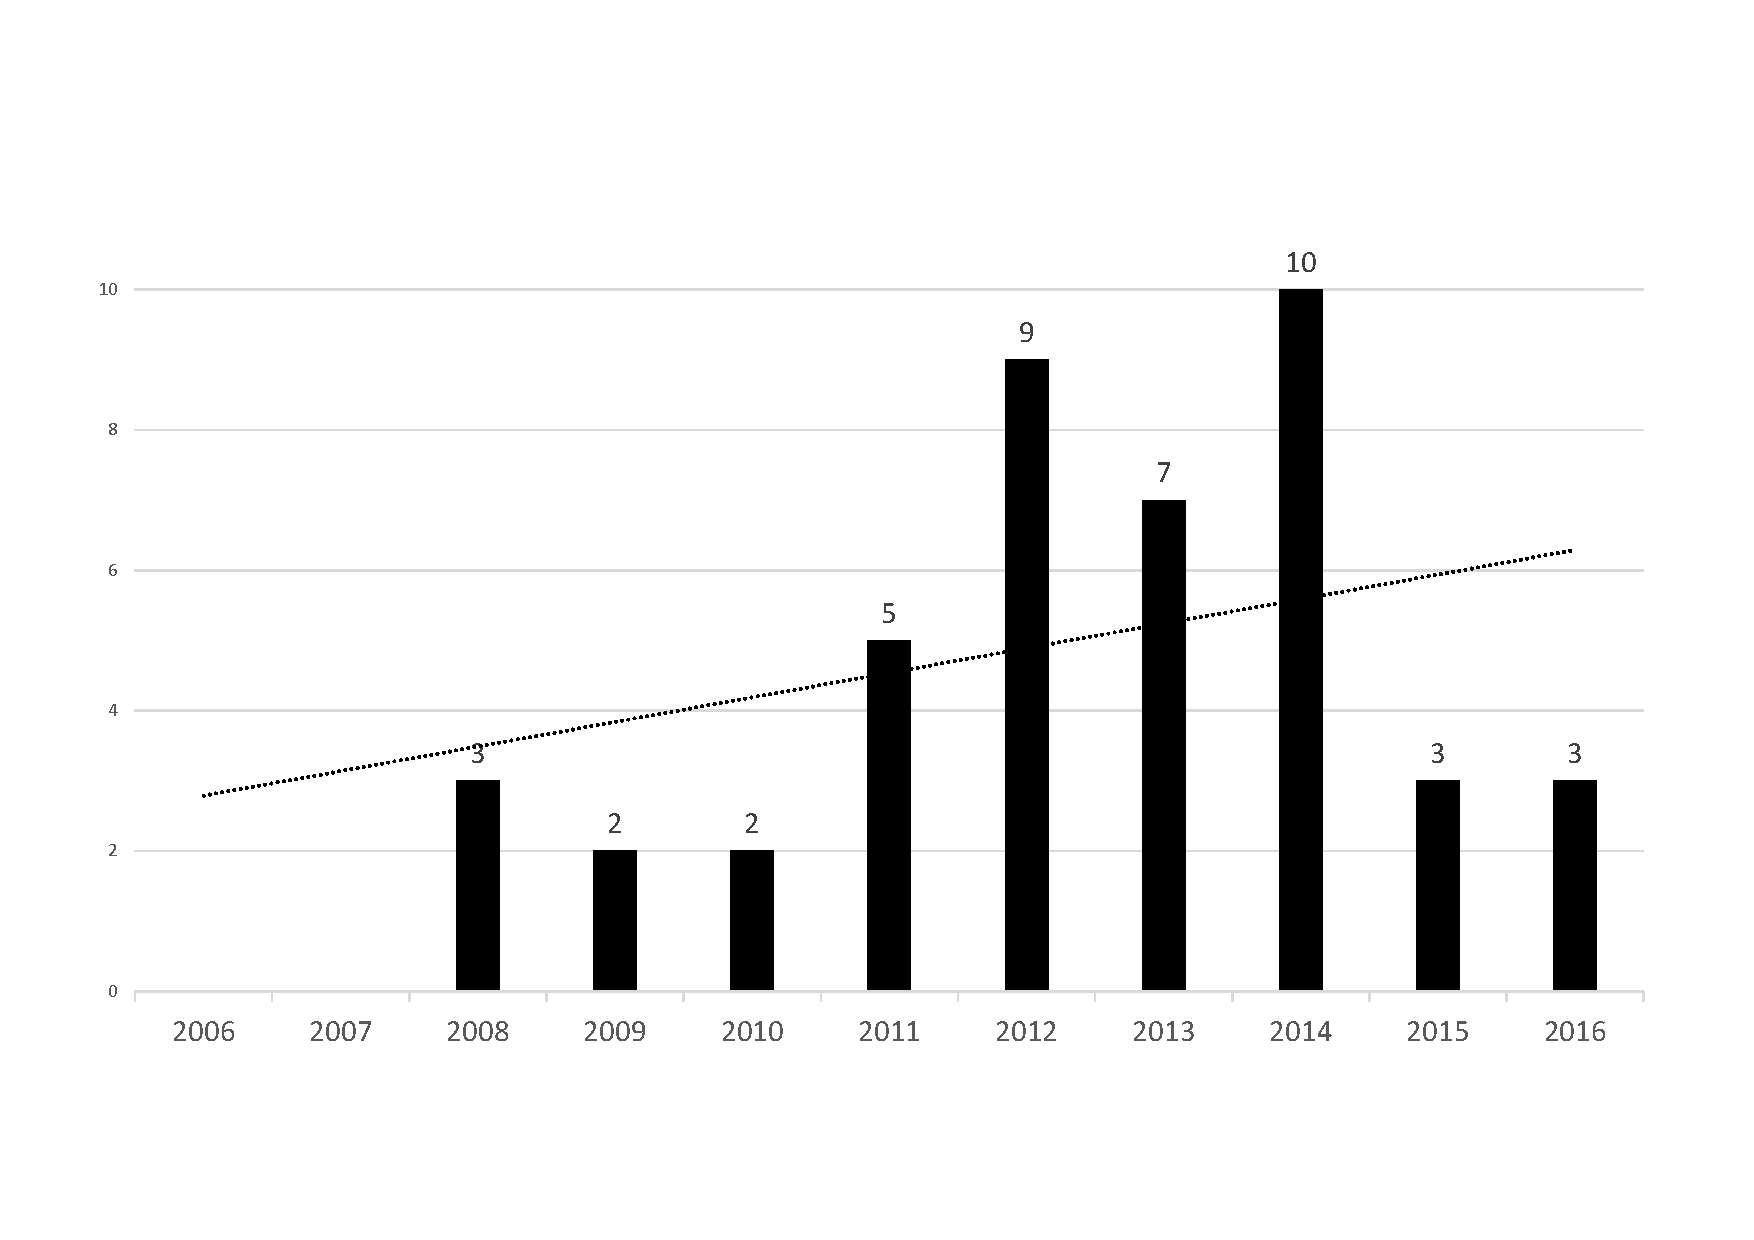
\includegraphics[scale=0.50]{quantidadeano.pdf}
	\caption{Distribuição de estudos por ano}
	\label{fig:qtdano}
\end{figure}

Com base na \ref{fig:qtdano}, observamos um número crescente de estudos ao longo dos anos. Especial atenção é dada a 2014 com 10 estudos. Além disso, com exceção de 2006 e 2007, sem ocorrência, os estudos são bem distribuídos na maioria dos anos, como em 2008, 2009, 2010, 2011, 2015 e 2016.

\subsubsection{Qualidade de Estudos}

Para garantir a qualidade mínima dos estudos, realizamos uma avaliação de qualidade conforme planejado na seção \ref{sec:extraction_process}, levando em consideração a aplicação dos critérios de qualidade da Seção \ref{sec:quality_analysis}.

Todos os estudos da Lista Final têm qualidade mínima com base em tais critérios, como podemos ver na  \ref{table:ranking} com a maioria das respostas `` Sim ''.

\begin{landscape}
	%\scalefont{0.6}	
	\tiny
	\begin{longtable}{c|c|c|c|c|c|c|c}
		\caption{Avaliação de Qualidade de Estudos}
		\label{table:ranking} \\\hline
		\textbf{ID do Estudo} &
		\textbf{QC.1-Propósito} &
		\textbf{QC.2-Compatibilidade} &
		\textbf{QC.3-Avaliação} &
		\textbf{QC.4-Coleção de dados} &
		\textbf{QC.5-Análise de dados} &
		\textbf{QC.6-Consistência dos Resultados} &
		\textbf{QC.7-Contribuição} 
		\\\hline \hline
		\endfirsthead
		%
		
		
		%		\multicolumn{8}{c}%
		%		{{\bfseries \tablename\\thetable{} continued from previous page}} \\
		%		\hline
		\textbf{ID do Estudo} &
		\textbf{QC.1-Propósito} &
		\textbf{QC.2-Compatibilidade} &
		\textbf{QC.3-Avaliação} &
		\textbf{QC.4-Coleção de dados} &
		\textbf{QC.5-Análise de dados} &
		\textbf{QC.6-Consistência dos Resultados} &
		\textbf{QC.7-Contribuição} 
		\\\hline \hline
		\endhead
		%
		S1 & Sim & Não & Sim & Sim & Sim & Sim & Sim \\\hline
		S2 & Sim & Não & Sim & Sim & Sim & Sim & Sim \\\hline
		S3 & Sim & Não & Sim & Sim & Sim & Sim & Sim \\\hline
		S4 & Sim & Não & Não Informado & Sim & Sim & Sim & Sim \\\hline
		S5 & Sim & Não & Não Informado & Não Informado & Não Informado & Sim & Sim \\\hline
		S6 & Sim & Não & Não Informado & Sim & Sim & Sim & Sim \\\hline
		S7 & Sim & Não & Sim & Sim & Sim & Sim & Sim \\\hline
		S8 & Sim & Não & Sim & Sim & Sim & Sim & Sim \\\hline
		S9 & Sim & Não & Sim & Sim & Sim & Sim & Sim \\\hline
		S10 & Sim & Não & Sim & Sim & Sim & Sim & Sim \\\hline
		S11 & Sim & Não & Não & Sim & Sim & Sim & Sim \\\hline
		S12 & Sim & Não & Sim & Sim & Sim & Sim & Sim \\\hline
		S13 & Sim & Sim & Não Informado & Sim & Sim & Sim & Sim \\\hline
		S14 & Sim & Não & Sim & Sim & Sim & Sim & Sim \\\hline
		S15 & Sim & Sim & Sim & Sim & Sim & Sim & Sim \\\hline
		S16 & Sim & Não & Não Informado & Sim & Sim & Sim & Sim \\\hline
		S17 & Sim & Não & Sim & Sim & Sim & Sim & Sim \\\hline
		S18 & Sim & Sim & Não Informado & Sim & Sim & Sim & Sim \\\hline
		S19 & Sim & Sim & Sim & Sim & Sim & Sim & Sim \\\hline
		S20 & Sim & Sim & Sim & Sim & Sim & Sim & Sim \\\hline
		S21 & Sim & Sim & Sim & Sim & Sim & Sim & Sim \\\hline
		S22 & Sim & Não & Sim & Sim & Sim & Sim & Sim \\\hline
		S23 & Sim & Sim & Sim & Sim & Sim & Sim & Sim \\\hline
		S24 & Sim & Sim & Não Informado & Sim & Sim & Sim & Sim \\\hline
		S25 & Sim & Sim & Sim & Sim & Sim & Sim & Sim \\\hline
		S26 & Sim & Sim & Sim & Sim & Sim & Sim & Sim \\\hline
		S27 & Sim & Sim & Sim & Sim & Sim & Sim & Sim \\\hline
		S28 & Sim & Sim & Sim & Sim & Sim & Sim & Sim \\\hline
		S29 & Sim & Sim & Sim & Sim & Sim & Sim & Sim \\\hline
		S30 & Sim & Não & Sim & Sim & Sim & Sim & Sim \\\hline
		S31 & Sim & Sim & Sim & Não Informado & Não Informado & Sim & Sim \\\hline
		S32 & Sim & Sim & Não Informado & Não Informado & Não Informado & Sim & Sim \\\hline
		S33 & Sim & Sim & Sim & Sim & Sim & Sim & Sim \\\hline
		S34 & Sim & Sim & Não Informado & Não Informado & Não Informado & Sim & Sim \\\hline
		S35 & Sim & Sim & Sim & Não Informado & Não Informado & Sim & Sim \\\hline
		S36 & Sim & Sim & Sim & Não Informado & Não Informado & Sim & Sim \\\hline
		S37 & Sim & Sim & Não & Não Informado & Não Informado & Sim & Sim \\\hline
		S38 & Sim & Sim & Sim & Sim & Sim & Sim & Sim \\\hline
		S39 & Sim & Sim & Sim & Sim & Sim & Sim & Sim \\\hline
		S40 & Sim & Sim & Sim & Sim & Sim & Sim & Sim \\\hline
		S41 & Sim & Não & Não Informado & Não Informado & Não Informado & Sim & Sim \\\hline
		S42 & Sim & Não & Sim & Sim & Sim & Sim & Sim \\\hline
		S43 & Sim & Sim & Sim & Sim & Sim & Sim & Sim \\\hline
		S44 & Sim & Não & Sim & Sim & Sim & Sim & Sim \\\hline		
	\end{longtable}
\end{landscape}

\subsection{Resultados em questões de pesquisa}

Nesta seção apresentamos os resultados com base em cada questão de pesquisa pré-definida.

\subsubsection{\bf{RQ.1:Para quais domínios do aplicativo LPS, tipos de solução e propostas TBM são usados?}}% 1 + 3 + 11

Para responder a essa pergunta, levamos em consideração o TBM aplicado a domínios LPS (por exemplo, software, automotivo), tipos de solução de área de pesquisa LPS (por exemplo, modelagem de recursos) e o tipo de proposta de estudos (por exemplo, abordagem, técnica, ferramenta).

Identificamos sete domínios de aplicação distintos nos quais o TBM for LPS é aplicado. \ref{table:qpp1} lista cada domínio e respectivos estudos e a \ref{fig:chart_domains} mostra o número de estudos por domínio.

\begin{table}[!h]
	\centering
	\scriptsize
	\caption{TBM de domínios de aplicativos LPS}
	\label{table:qpp1}
	\begin{tabular}{l|l|c}
		\hline
		\textbf{Domínio de Aplicação} & \textbf{ID do Estudo} & \textbf{Count}\\\hline \hline
		Aeroespacial     		& S5, S8 & 02\\\hline
		Automotivo       	& S1, S3, S4, S7, S10, S11, S16, S17, S30 & 09\\\hline
		Eletrônico       	& S2, S9, S42, S44 & 04\\\hline
		Fabricação     & S6 & 01\\\hline
		Medicina         	& S41 & 01\\\hline
		Software         	& \begin{tabular}[c]{@{}l@{}l@{}}T13, S15, S18, S19, S20, S21, S23, S24, S25,\\S26, S27, S28, S29, S31, S32, S33, S34, S35,\\T36, S37, S38, S39, S40, S43\end{tabular} & 24\\\hline
		Telecomunicação & S12, S14, S22 & 03\\\hline \hline
		
		\multicolumn{2}{c|}{\textbf{TOTAL}} & \textbf{44} \\\hline
		
	\end{tabular}
\end{table}

\begin{figure}[!h]
	\centering	
	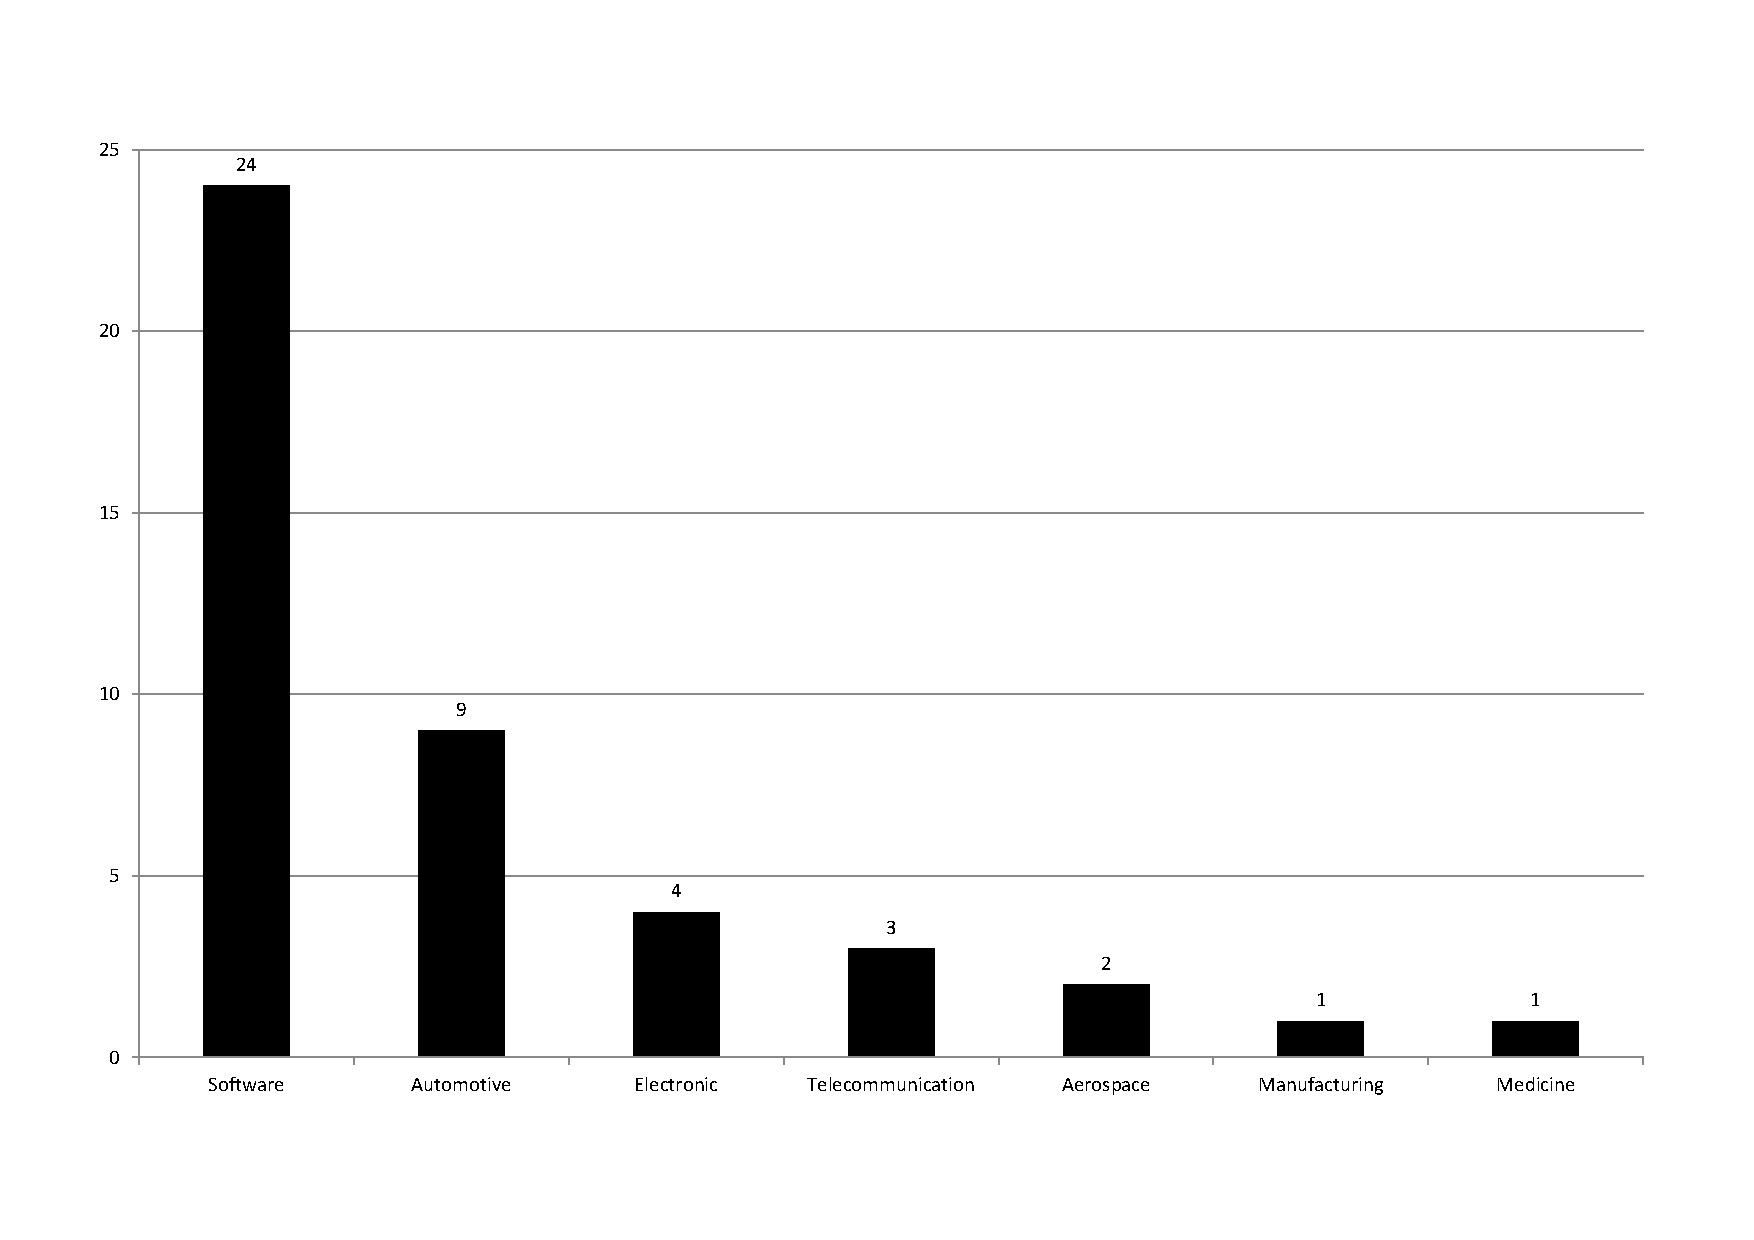
\includegraphics[scale=0.50]{chart_domains.pdf}
	\caption{Automação TBM para LPS de abordagens de teste}
	\label{fig:chart_domains}
\end{figure}

O domínio de aplicação \textit{Software} tem a maioria das ocorrências com 24 estudos, seguido por \textit{Automotive} com nove, que utiliza software embutido em seus produtos.

\paragraph{\textbf{Aerospacial}}

MPLM é uma das poucas ferramentas que concentram o maior esforço na questão da solução de variabilidade na geração de casos de teste, \citet{samih2014mplm} em seu recurso de estudo a ferramenta Matelo, juntamente com outras ferramentas permite derivar a variante do modelo a partir de um o conjunto desejado e, assim, gerar casos de teste para um projeto experimental na Airbus defense \& Space. O TBM auxilia na reutilização para geração dos casos de teste, o outro estudo que trabalha no mesmo domínio é uma extensão deste citado.

\paragraph{\textbf{Automotivo}}

\citet{Lity_et_al2012} apresenta a abordagem delta, que trabalha com elementos cruzados de um elemento chamado G, onde os casos de teste são definidos com uma cobertura satisfatória. Os artefatos de teste são desenvolvidos de forma incremental à medida que surgem novas variantes de produtos. Consideramos que o fator de regressão e a adaptabilidade dos artefatos de teste podem ter uma contribuição significativa ao serem trabalhados em um LPS, embora não tenham enfoque no TBM. O uso de software embarcado em produtos automotivos cresce exponencialmente, o TBM tem ajudado a gerar os testes desses produtos que sofrem variações, onde existe um núcleo central, e cada variação pode ou não conter uma especificidade única das demais.

\paragraph{\textbf{Eletrônico}}

Seguindo esse conceito \citet{Steffens_et_al2012} usa modelos para gerar subgrupos ou casos de teste desses modelos, aborda a questão da interação de recursos com a cobertura de teste e gerencia as variabilidades como itens cruzados. MoSo-PoLiTe, uma ferramenta que propõe fazer a derivação dos produtos a partir do modelo principal, utilizando o teste combinatório automatizado. O TBM atua na geração de casos de teste para subgrupos de produtos, além de buscar garantir uma maior cobertura de erros de funcionalidade, já que se trata de um domínio eletrônico, a garantia de qualidade deve ser com uma margem significativamente maior.

\paragraph{\textbf{Fabricação}}

\citet{knapp2014use} apresenta um procedimento associado a um conjunto de ferramentas para atribuir o resultado de um caso de teste a um membro arbitrário de um LPS, usando modelos de variabilidade baseados em UML e CVL, o modelo é usado para a criação de máquinas de estado são então convertidos em diagrama de classes.

\paragraph{\textbf{Medicina}}

\citet{hasling2008model} realiza a conversão dos modelos em diagramas de atividades e caso de uso, após esta conversão é elaborada a criação de casos de teste, onde as variantes dos modelos podem ser consideradas como variáveis. Ao usar o TBM, ele não menciona se a variabilidade é manipulada, simplesmente usada para criar casos de teste a partir de diagramas de atividades.

\paragraph{\textbf{Software}}

O software é um dos domínios mais relatados, inicialmente porque está diretamente ligado ao tópico de pesquisa, embora os demais domínios também utilizem o TBM no processo de desenvolvimento de algum produto de software específico para um determinado domínio.

\citet{Olimpiew2008} também fornece muitos dados e informações sobre TBM em LPS, embora o foco seja em diagramas de atividades customizados, mas com foco na reutilização do teste em produtos de variante LPS. A abordagem proposta do CADeT transforma os casos de uso em diagramas de atividades, que por sua vez são transformados em casos de teste. As especificações de teste são rastreadas a partir do diagrama de atividades e do caso de uso.

A grande maioria dos estudos relata a criação de alguma abordagem ou ferramenta em TBM para auxiliar no desenvolvimento de LPS, no entanto, muitos não relatam com mais detalhes o uso de TBM em seu estudo.

\paragraph{\textbf{Telecomunicação}}

O TBM atua no auxílio da derivação de casos de teste de máquinas de estado, o desempenho neste domínio é devido ao uso de mídia embutida nos dispositivos de comunicação. Em um dado momento é possível interpretar que o estudo referente a esse domínio seria manufatura, mas tem uma área de atuação bem definida que seria a divisão de pesquisa de uma grande empresa de telecomunicações.

Ainda sobre o uso de ferramentas \citet{wang2013automated} retrata o uso de um processo automatizado de seleção de teste de forma mínima e sistematizado. Processos automatizados contribuem para algoritmos de seleção, por mais que estejam em uma manufatura, para criar uma visão sistêmica da seleção de variabilidade.

% ================= tipos de solução inicio

A \ref{tab:spl_solutions} lista os estudos realizados para testar diferentes tipos de solução de LPS, como:\textit{Teste de recurso}, \textit{Teste de modelo LPS} e \textit{Teste PLA} (arquitetura de linha de produto - PLA). Para essa classificação, separamos o PLA dos artefatos gerais do LPS, devido à importância direta do PLA para o sucesso dos LPSs.

\begin{table}[!h]
	\centering
	\caption{Teste de TBM de tipos de solução LPS}
	\scriptsize
	\label{tab:spl_solutions}
	\begin{tabular}{l|l|c}
		\hline
		\textbf{Tipo de Solução} 			& \textbf{ID do estudo} 	& \textbf{Estudos} \\\hline \hline
		
		Feature Testing 			& S1, S8, S11, S14, S15, S17, S18, S26, S27, S29, S32 & 11 \\\hline
		
		LPS Model Testing 		& \begin{tabular}[c]{@{}l@{}}T2, S3, S4, S5, S9, S12, S13, S19, S20, S21, S24, S30, \\S36, S37, S39\end{tabular} 																				& 15\\\hline
		
		PLA Testing						& \begin{tabular}[c]{@{}l@{}}T6, S7, S10, S16, S22, S23, S25, S28, S31, S33, S34, \\S35, S38, S40, S41, S42, S43, S44\end{tabular} 														& 18 \\\hline \hline
		
		\multicolumn{2}{c|}{\textbf{TOTAL}} & \textbf{44} \\\hline
	\end{tabular}
\end{table}

Podemos observar na \ref{tab:spl_solutions} a maioria dos estudos voltados para o teste de PLA. Isso ocorre principalmente devido ao papel central do PLA para o desenvolvimento de LPSs, uma vez que é uma abstração de todos os potenciais produtos únicos a serem desenvolvidos por um LPS. Portanto, 18 estudos (40,9 \%) testaram o PLA e seus modelos. Os testes de PLA estão no nível de dados de entrada e saída, por meio de testes de caixa preta e testes de funcionalidade. Ao buscar a reutilização, há uma preocupação com a confiabilidade da arquitetura principal e com a derivação de produtos LPS. % \textcolor{red}{COMO OS ESTUDOS TEM FEITO TESTE DE PLA? DESCREVER GERAL E SUCINTAMENTE ...}

Com relação ao teste de modelos de LPS, encontramos 34 \% dos estudos levando em consideração qualquer tipo de nível de teste ou tipo para LPSs para engenharia de domínio e engenharia de aplicação. Testar modelos de LPS é um meio de fornecer reutilização de casos de teste para produtos específicos derivados de um LPS. Como apontado na literatura geral de testes, a detecção de defeitos nos modelos pode ser várias vezes menos custosa do que nas atividades posteriores do NPS. O teste nos modelos de LPS depende muito de qual nível será testado. Na maioria desses estudos, os testes dependem de funcionalidades, portanto, os modelos estão sendo testados de acordo com o resultado esperado dos requisitos especificados. % \textcolor{red}{COMO OS ESTUDOS TEM FEITO TESTE DE MODELOS DE LPS? DESCREVER GERAL E SUCINTAMENTE ...}

O teste de recursos é composto por 25 \% dos estudos. Embora os recursos estejam no nível do espaço do problema, seus testes são essenciais para o sucesso de um LPS, pois os recursos estão diretamente relacionados aos modelos de LPS em todos os níveis, incluindo o código-fonte. O teste de recurso funcional está de acordo com a cobertura das ações esperadas. Assim, este é um grande desafio, pois com a derivação de novos produtos suas funcionalidades podem sofrer variações, o que pode causar uma combinação exponencial de sequências de teste. % \textcolor{red}{COMO OS ESTUDOS TEM FEITO TESTE DE recursos? DESCREVER GERAL E SUCINTAMENTE ...}

% ================= fim soluções


% ================= inicio soluções 2

Por uma questão de contribuições de estudos, analisamos e apresentamos na \ref{table:contribuicao} em termos de seus tipos de propostas.

\begin{table}[!h]
	\centering
	\scriptsize
	\caption{Propostas principais de TBM para LPS}
	\label{table:contribuicao}
	\begin{tabular}{l|l|c}
		\hline
		
		\textbf{Tipo de proposta} & \textbf{ID do estudo} &  \textbf{Estudos}\\\hline \hline
		
		Abordagem & \begin{tabular}[c]{@{}l@{}}T1, S5, S6, S7, S8, S9, S10, S11, S13, S14, S15, S16,\\S17, S18, S20, S21, S22, S23, S24, S27, S28, S29,\\S30, S31, S35, S36, S37, S38, S39, S41, S42, S43, S44\end{tabular} & 33 \\\hline
		
		Algoritmo & S3, S25, S26 & 03 \\\hline
		
		Kit de ferramentas & S40  & 01 \\\hline
		
		Estratégia & S33  & 01 \\\hline
		
		Abordagem de Extensão & S12  & 01 \\\hline
		
		Ferramenta & S2, S4, S34  & 03 \\\hline
		
		Metodologia & S19  & 01 \\\hline
		
		Tutorial & S32  & 01 \\\hline \hline
		
		\multicolumn{2}{c|}{\textbf{TOTAL}} & \textbf{44} \\\hline
	\end{tabular}
\end{table}

Podemos observar que a maioria dos estudos (33) apresenta como uma contribuição de proposta uma abordagem. Os estudos restantes relatam de uma a três propostas cada.

\subsubsection{\bf{RQ.2:Quais abordagens de TBM, níveis de teste, artefatos, ferramentas e modelos foram usados para testar LPSs?}}

Nesta seção, fornecemos resultados sobre abordagens, níveis de teste, artefatos, ferramentas e modelos usados para aplicar o TBM às LPSs.

Os estudos analisados realizam principalmente testes de tempo de projeto. Além disso, para esta questão de pesquisa, analisamos os testes:abordagens, níveis e tipos e automação.

\paragraph{\textbf{Abordagens Usadas}}

A partir de estudos selecionados, criamos duas abordagens baseadas em "caixa":caixa branca e caixa preta. O primeiro é quando alguém tem acesso ao código-fonte e pode fornecer análises com maior profundidade. Este último é realizado quando não se tem acesso ao código, mas apenas para inserir dados e parâmetros, assim como os resultados produzidos.

\ref{tab:test_approaches} apresenta os estudos classificados em cada uma das abordagens.

\begin{table}[!h]
	\centering
	\scriptsize
	\caption{Abordagens de TBM para LPS}
	\label{tab:test_approaches}
	\begin{tabular}{l|l|c}
		\hline
		\textbf{Abordagem de Teste} & \textbf{ID do estudo} & \textbf{Estudos}\\\hline \hline
		
		Caixa-Preta  		& \begin{tabular}[c]{@{}l@{}}S2, S3, S7, S8, S9, S10, S11, S12, S13, S14, S15, S16,\\S17, S18, S19, S21, S22, S23, S24, S25, S26, S27, S28,\\S29, S30, S31, S32, S33, S34, S35, S36, S37, S38, S39,\\S40, S41, S42, S43, S44\end{tabular} & 39 \\\hline
		
		Caixa-Branca 		& S1, S4, S20 & 03 \\\hline
		
		Não Informado	& S5, S6	& 02 \\\hline \hline
		
		\multicolumn{2}{c|}{\textbf{TOTAL}} & \textbf{44} \\\hline
	\end{tabular}
\end{table}

Podemos observar que a maioria dos estudos (39/44) executa testes de caixa preta, principalmente porque:os testes são realizados em uma abstração de nível superior, como, por exemplo, testes funcionais; e LPS na atividade de engenharia de domínio.

A grande maioria dos estudos procura gerar casos de teste por meio de modelos, portanto, esse é um dos fatores que levam ao uso da abordagem da caixa preta. \citet{Steffens_et_al2012} use modelos para gerar casos de teste. Esta prática é feita por quase todos os outros estudos \cite{cichos2011model, oster2011pairwise, samih2014deriving, lackner2014model, Garcia_et_al2010}.


\paragraph{\textbf{Níveis de teste}}

Encontramos diferentes níveis e tipos de testes TBM. Da Lista Final, quatro estudos se destacam mais (\ref{tab:test_levels} \footnote{Um estudo pode suportar mais de um nível ou tipo de teste.}), Que são:\textit{Integração}, \textit{Sistema }, \textit{Regressão} e \textit{Funcional}. A \ref{fig:chart_levels_types} descreve os níveis e tipos de TBM de LPSs.

\begin{table}[!h]
	\centering
	\scriptsize
	\caption{TBM dos níveis e tipos de testes de LPS}
	\label{tab:test_levels}
	\begin{tabular}{l|l|c}
		\hline
		\textbf{Nível / Tipo de Teste} & \textbf{ID do estudo} & \textbf{Estudos}\\\hline \hline
		
		%model testing
		Combinação     & S4 					& 01			\\\hline
		
		%levels - black-box		
		Estrutural      & S20						& 01	\\\hline
		
		Funcional		  & S6, S9, S10, S22, S24, S28, S31 
		& 07 \\\hline
		
		Performance     & S20 					& 01	\\\hline
		
		%levels - white-box		
		Regressão      & \begin{tabular}[c]{@{}l@{}}S1, S11, S13, S14, S15, S17, S18, S27, S30,\end{tabular}                                  		& 09	\\\hline
		
		Sistema          & \begin{tabular}[c]{@{}l@{}}S25, S26, S33, S34, S35, S36, S38, S39, S40, S41,\\S42, S43, S44\end{tabular}  & 13      \\\hline
		
		Integração     & \begin{tabular}[c]{@{}l@{}}S3, S5, S7, S8, S11, S13, S14, S15, S16, S17, S18,\\S19, S21, S23, S29, S37  \end{tabular} 																		& 16	\\\hline
		
		Unitário	          & S2					& 01			\\\hline
		
		
		Não Informado    & S12, S32		& 02	\\\hline \hline
		
		\multicolumn{2}{c|}{\textbf{TOTAL}} & \textbf{51} \\\hline
	\end{tabular}
\end{table}

\begin{figure}[!h]	
	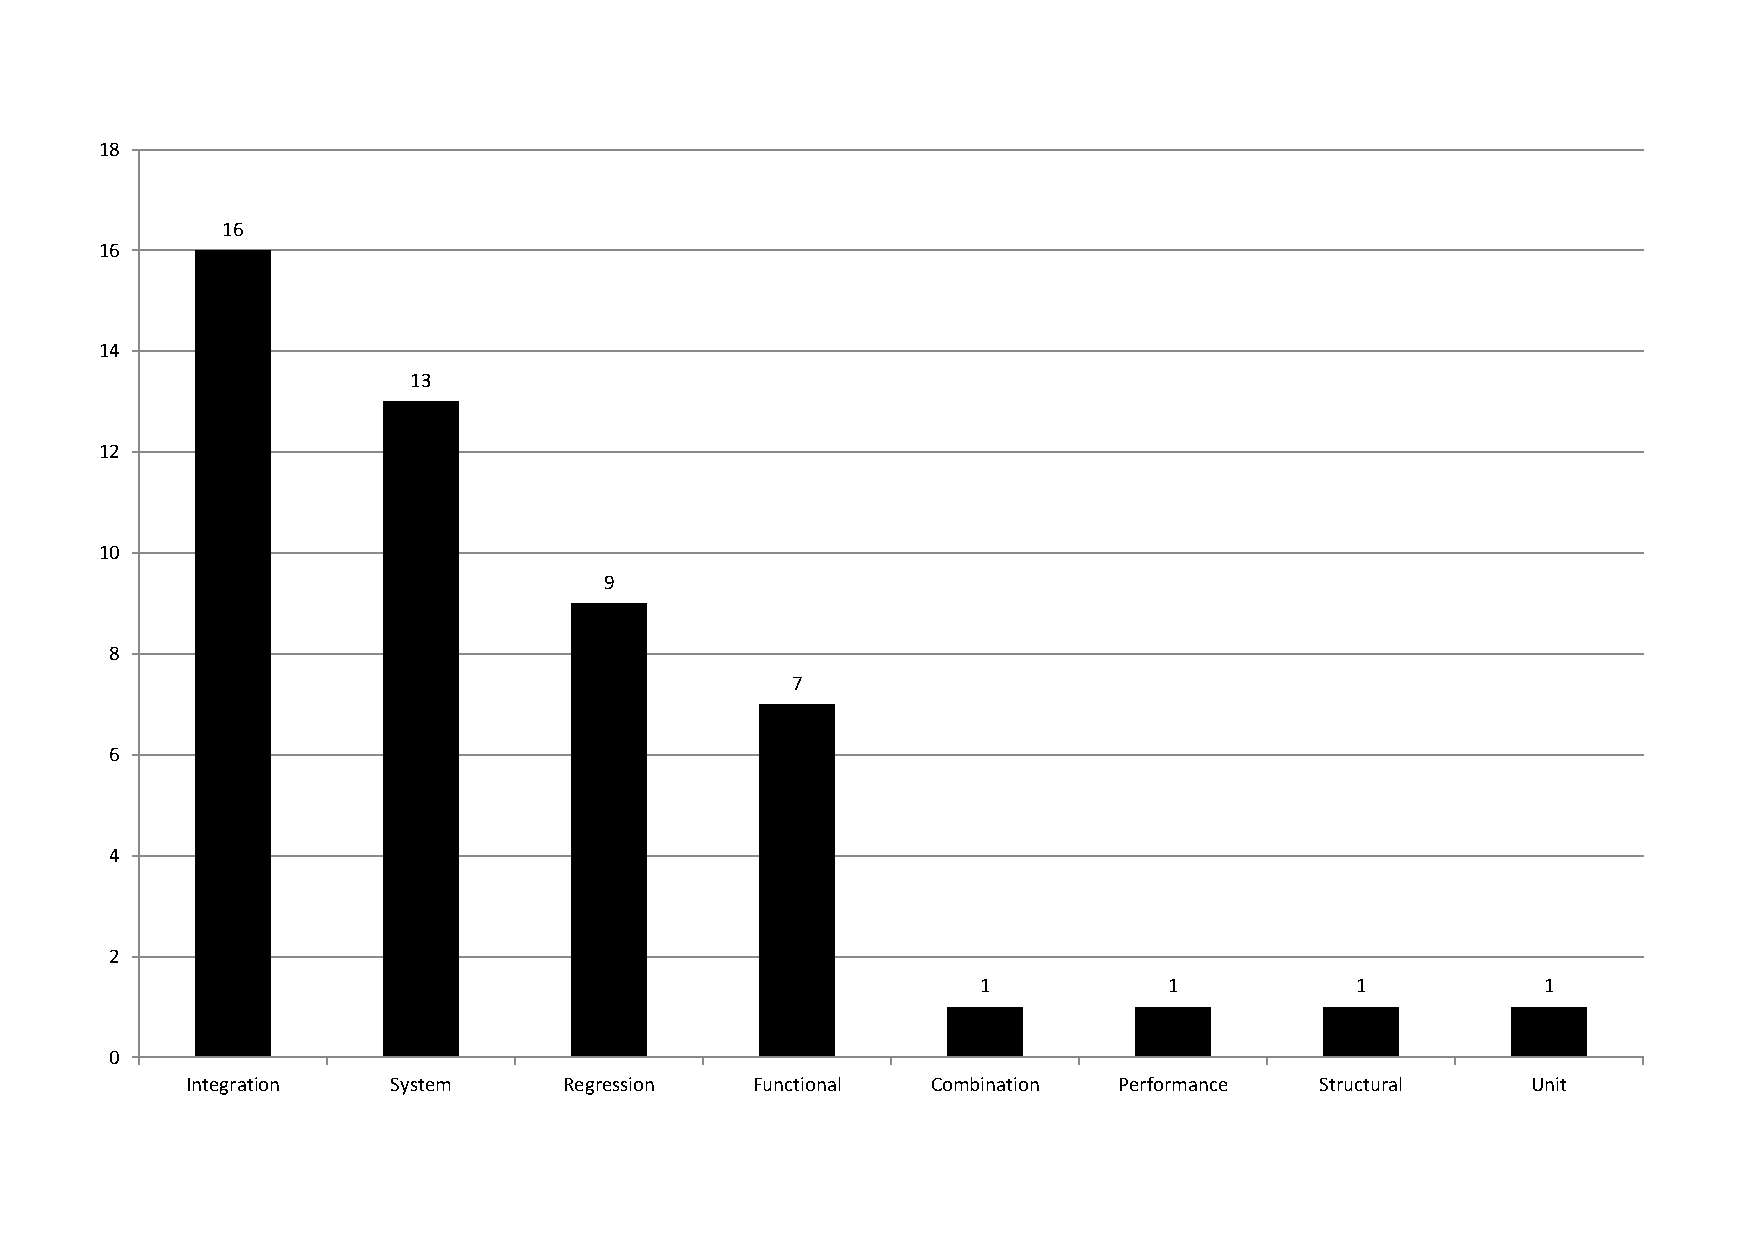
\includegraphics[scale=0.50]{chart_levels_types.pdf}
	\caption{Comparação de níveis e tipos de TBM para LPS}
	\label{fig:chart_levels_types}
\end{figure}

Podemos observar que o nível de teste de integração é um dos mais considerados, pois a maioria dos testes é realizada na engenharia de domínio LPS. Além disso, para a reutilização de muitos casos de teste, a derivação de novos produtos requer uma verificação de integração entre modelos \cite{samih2014mplm, oster2011pairwise, samih2014deriving, oster2012feature, olimpiew2005model, cichos2011model, devroey2014coverage, varshosaz2015delta, samih2012relating, dukaczewski2013requirements, Garcia_et_al2010, wang2013automated, devroey2014behavioural, cai2013model} .

%Outros estudos visualizam algo semelhante, mas não funcionam de maneira modular. Eles buscam testes no nível do sistema, pois alguns deles afirmam que é muito caro lidar com uma grande quantidade de sequências de teste na engenharia de domínio do LPS. Portanto, eles só se concentram na estrutura do sistema \citet{devroey2012vision,devroey2014abstract,lochau2012parameterized,devroey2015vibes,beohar2014spinal,lackner2014model,weissleder2014avaliação,henard2013assessing,perrouin2010automated,hasling2008model,rodrigues2013plets}.

%Diferentes níveis de teste são cobertos por esses estudos, como Combinação, Estrutural, Funcional, Desempenho, Regressão e Unidade. Estes estudos preocupam-se com o nível de cobertura das funcionalidades e com a geração dos casos de teste de maneiras específicas como, por exemplo, os modelos knapp2014use, gebizli2016model, lackner2014model, dukaczewski2013, garcia2010automated, wang2013automated, lochau2012model, cai2013model, ali2012product, patel2015automated}.

\paragraph{\textbf{Automação de Testes}}

Ao analisar os estudos selecionados, identificamos o uso de ferramentas totalmente automatizadas e semi-automatizadas para auxiliar no teste de TBMs de LPSs. Também identificamos estudos sem auxílio de ferramentas, desenvolvendo manualmente atividades de testes, como podemos observar na \ref{tab:test_automation}.

\begin{table}[!h]
	\centering
	\scriptsize
	\caption{TBM de automação LPS}
	\label{tab:test_automation}
	\begin{tabular}{l|l|c}
		\hline
		\textbf{Abordagem de automação} & \textbf{ID do estudo}  & \textbf{Estudos}  \\\hline 
		
		Totalmente automatizado   		& \begin{tabular}[c]{@{}l@{}}S2, S3, S4, S5, S6, S7, S8, S9, S10, S11, \\S12, S13, S14, S15, S16, S17, S18, S20, \\S22, S23, S24, S26, S27, S28, S31, S40, S41  \end{tabular} & 27 \\\hline
		
		Semi-automatizado	& \begin{tabular}[c]{@{}l@{}} S19, S21, S25, S29, S30, S34, S36, S37, S38, S39,\\S42, S43, S44\end{tabular} & 13 \\\hline
		
		Manual					& S1, S33, S35 & 03 \\\hline
		
		Não Informado 		& S32  & 01 \\\hline \hline
		
		\multicolumn{2}{c|}{\textbf{TOTAL}} & \textbf{44} \\\hline
	\end{tabular}
\end{table}

Nãos estudos selecionados, verificamos o uso de ferramentas \textit{fully-automated} em atividades de teste. Segundo estudos selecionados, a maioria deles utiliza algum tipo de automação para realizar tais atividades. As ferramentas usadas são amplamente implementadas pelos autores dos estudos \cite{oster2011moso, Steffens_et_al2012, devroey2015vibes, perrouin2010automated}, mas esses autores também fornecem comparações entre ferramentas de abordagens semelhantes \cite{oster2011moso, Steffens_et_al2012, devroey2015vibes, perrouin2010automated, rodrigues2013plets}.

Outro conjunto de estudos selecionados usa ferramentas \textit{semi-automated}, nas quais apenas um trecho do processo de teste é automatizado, com ou sem atividades manuais. O Olimpiew \cite{olimpiew2005model} cria casos de uso para permitir especificações de casos de teste reutilizáveis pelo arquiteto de software. De acordo com Weissleder e Lackner \cite{weissleder2013top}, os modelos são usados em conjunto para modelar recursos e comportamento para a geração de diagramas de máquinas de estado e comportamento por engenheiros de software usando abordagens semi-automatizadas.

Estudos puramente manuais não adotam nenhum tipo de automação das atividades de teste. Tais estudos discutem abordagens teóricas relacionadas com TBM de LPS e, portanto, foram classificados como \textit{Manual}. Em geral, as atividades manuais seriam a conversão de um modelo inicial em um modelo secundário com maior detalhe, depois para casos de teste \cite{lity2016applying, lochau2012parameterized, beohar2014spinal}. As abordagens manuais tendem a apresentar apenas conceitos teóricos do modelo de processo desenvolvido, ou buscam apresentar a essência referente a um contexto específico.

O gráfico de bolha da \ref{fig:approachXautomation} mostra a automação de abordagens. Como podemos observar, o teste caixa-preta tem maior automação, tanto por ferramentas totalmente automatizadas quanto semi-automatizadas, totalizando 39 estudos. As abordagens de caixa branca são menos executadas com o auxílio de ferramentas (semi) automatizadas, apenas três estudos.


\begin{figure}[!h]	
	\centering
	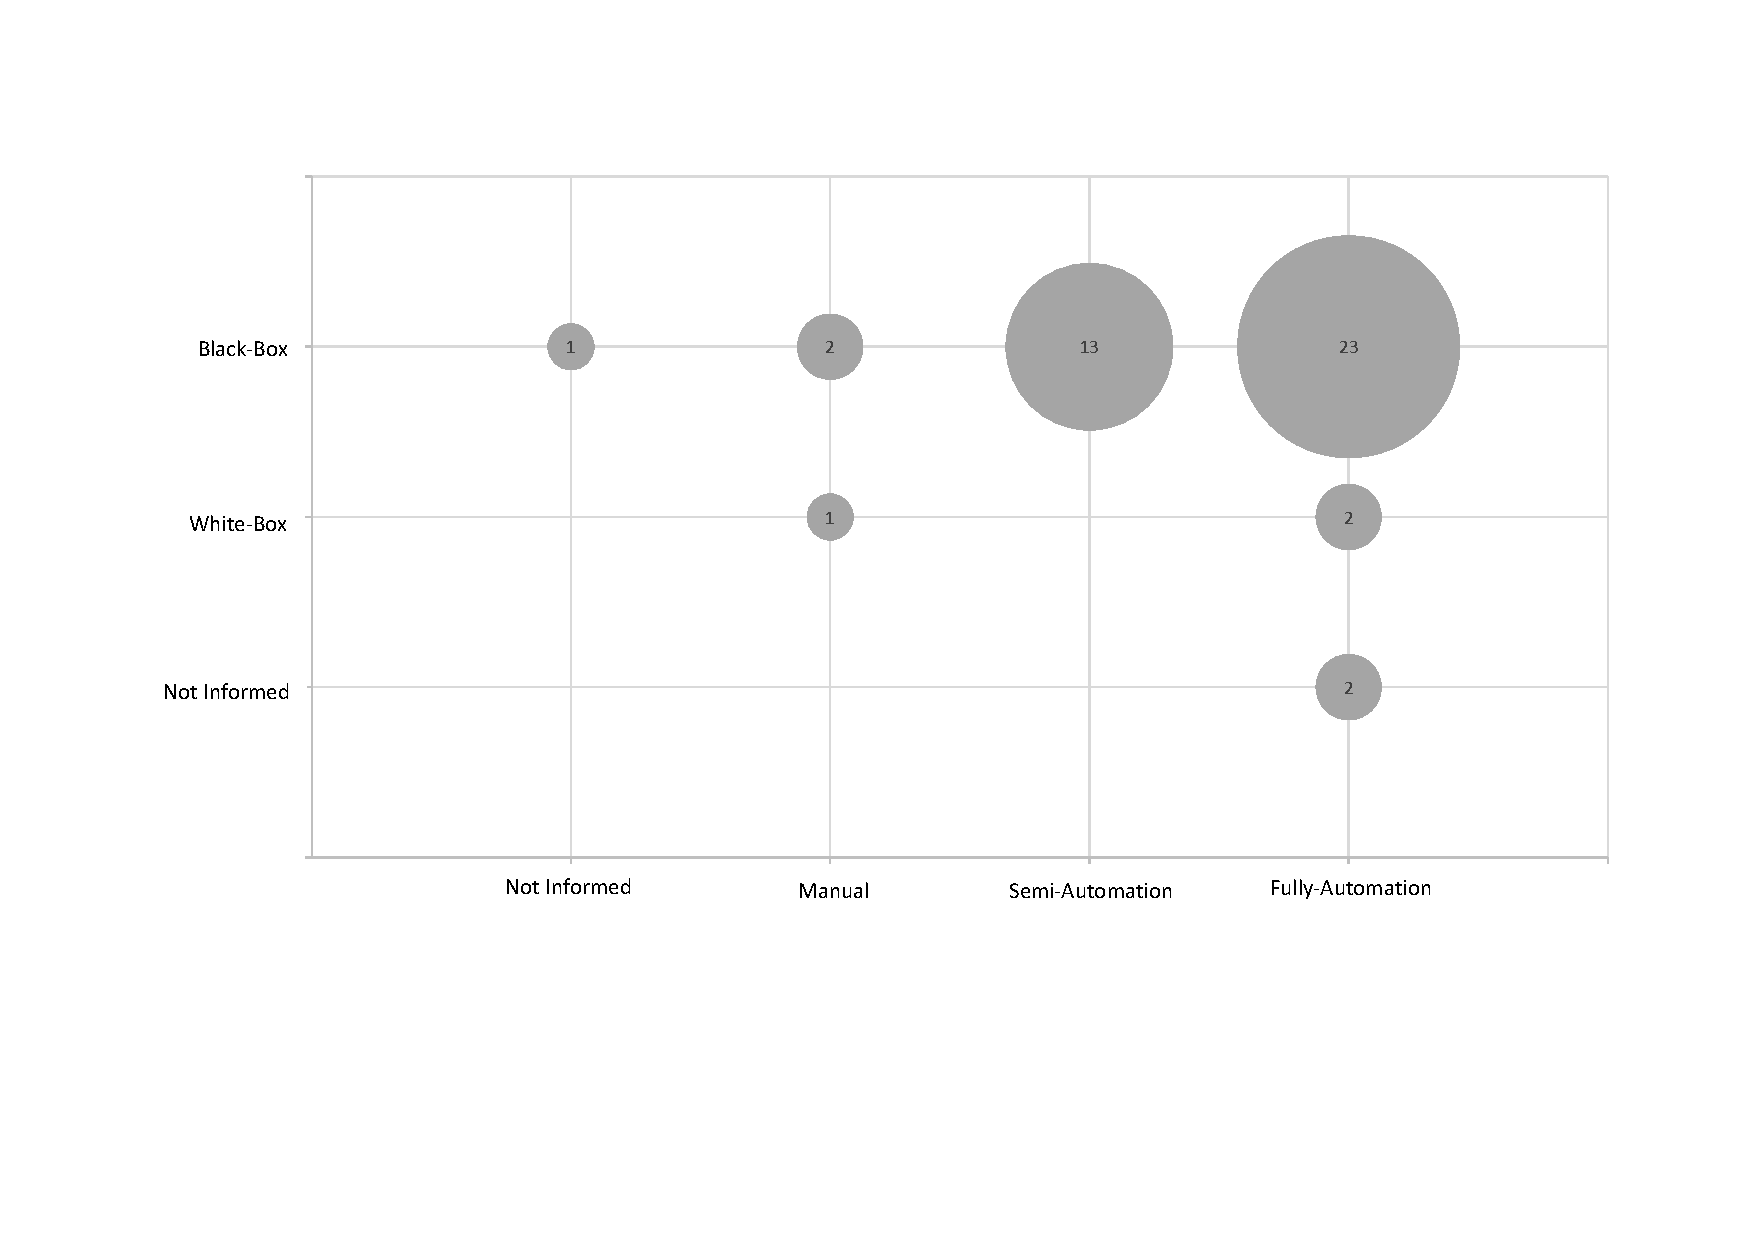
\includegraphics[scale=0.55]{bubble_approachXautomation.pdf}
	\caption{Automação TBM para LPS de abordagens de teste}
	\label{fig:approachXautomation}
\end{figure}

O gráfico de bolha da \ref{fig:teste_levelxautomation} mostra a automação dos níveis e tipos de teste.

\begin{figure}[!h]
	\centering	
	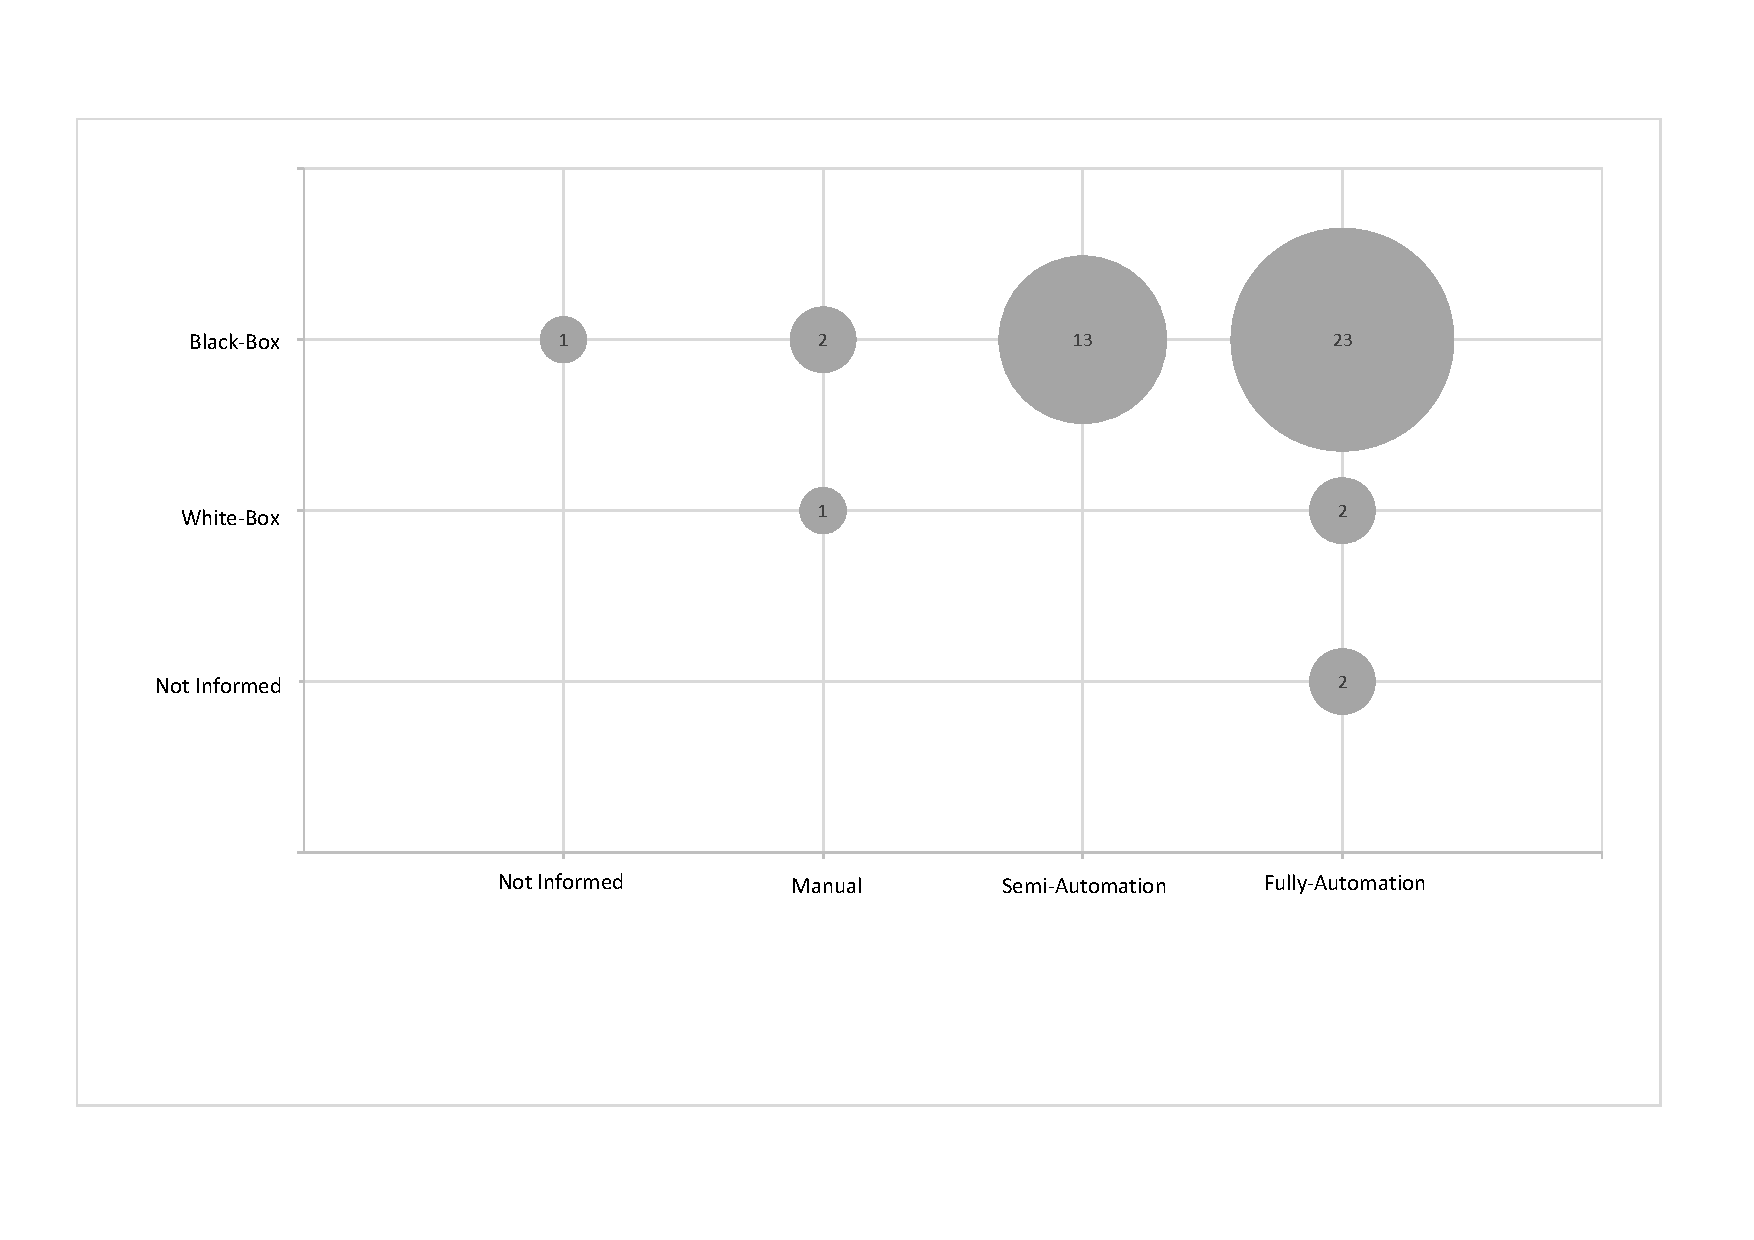
\includegraphics[scale=0.55]{bubble_Teste_level_automation.pdf}
	\caption{Automação de níveis de teste de TBM para LPS}
	\label{fig:teste_levelxautomation}
\end{figure}

Treze estudos são menos realizados com o auxílio de ferramentas (semi) automatizadas. Apenas três estudos não apresentam nenhum tipo de automação, enquanto um estudo não relata.


\paragraph{\textbf{Artefatos Usados}}

Para gerar casos de teste, os estudos de TBM usam vários artefatos diferentes, como Máquina de estados, Diagrama de classes, Diagrama de sequência e Modelo de recursos, como podemos observar na \ref{tab:artefatosutilizados}. Uma comparação de tais artefatos é fornecida na \ref{fig:chart_artifacts}.

\begin{table}[!h]
	\centering
	\scriptsize
	\caption{Artefatos Usados Durante TBM de LPS}
	\label{tab:artefatosutilizados}
	\begin{tabular}{l|l|c}
		\hline
		\textbf{Artefato} & \textbf{ID do estudo} & \textbf{Estudos} \\\hline \hline
		
		Máquina de Estado & \begin{tabular}[c]{@{}l@{}} S1, S6, S7, S10, S11, S12, S13, S14, S15, S17, S21,\\T22, S23, S27, S29, S30, S34, S38, S44\end{tabular} & 19 \\\hline
		
		Modelo original & S8, S9, S42 & 03\\\hline
		
		\begin{tabular}[c]{@{}l@{}}OVM Variability\\Model\end{tabular} & S8 & 01 \\\hline
		
		Diagrama de Classes & S6, S12, S14, S31 & 04 \\\hline
		
		Diagrama de atividades & S18, S19, S41 & 03 \\\hline
		
		Diagrama de casos de uso & S20, S28, S41, S43 & 04 \\\hline
		
		Diagrama de sequência & S24, S31, S36 & 03 \\\hline
		
		Diagrama de Transição & S7, S15, S25, S26, S33, S35, S37 & 07 \\\hline
		
		Diagrama de Funções & S2, S3, S4, S5, S9, S16, S39, S40 & 08 \\\hline
		
		Não Informado & S32 & 01 \\\hline \hline		
		
		\multicolumn{2}{c|}{\textbf{TOTAL}} & \textbf{53} \\\hline
	\end{tabular}
\end{table}

\begin{figure}[!h]
	\centering	
	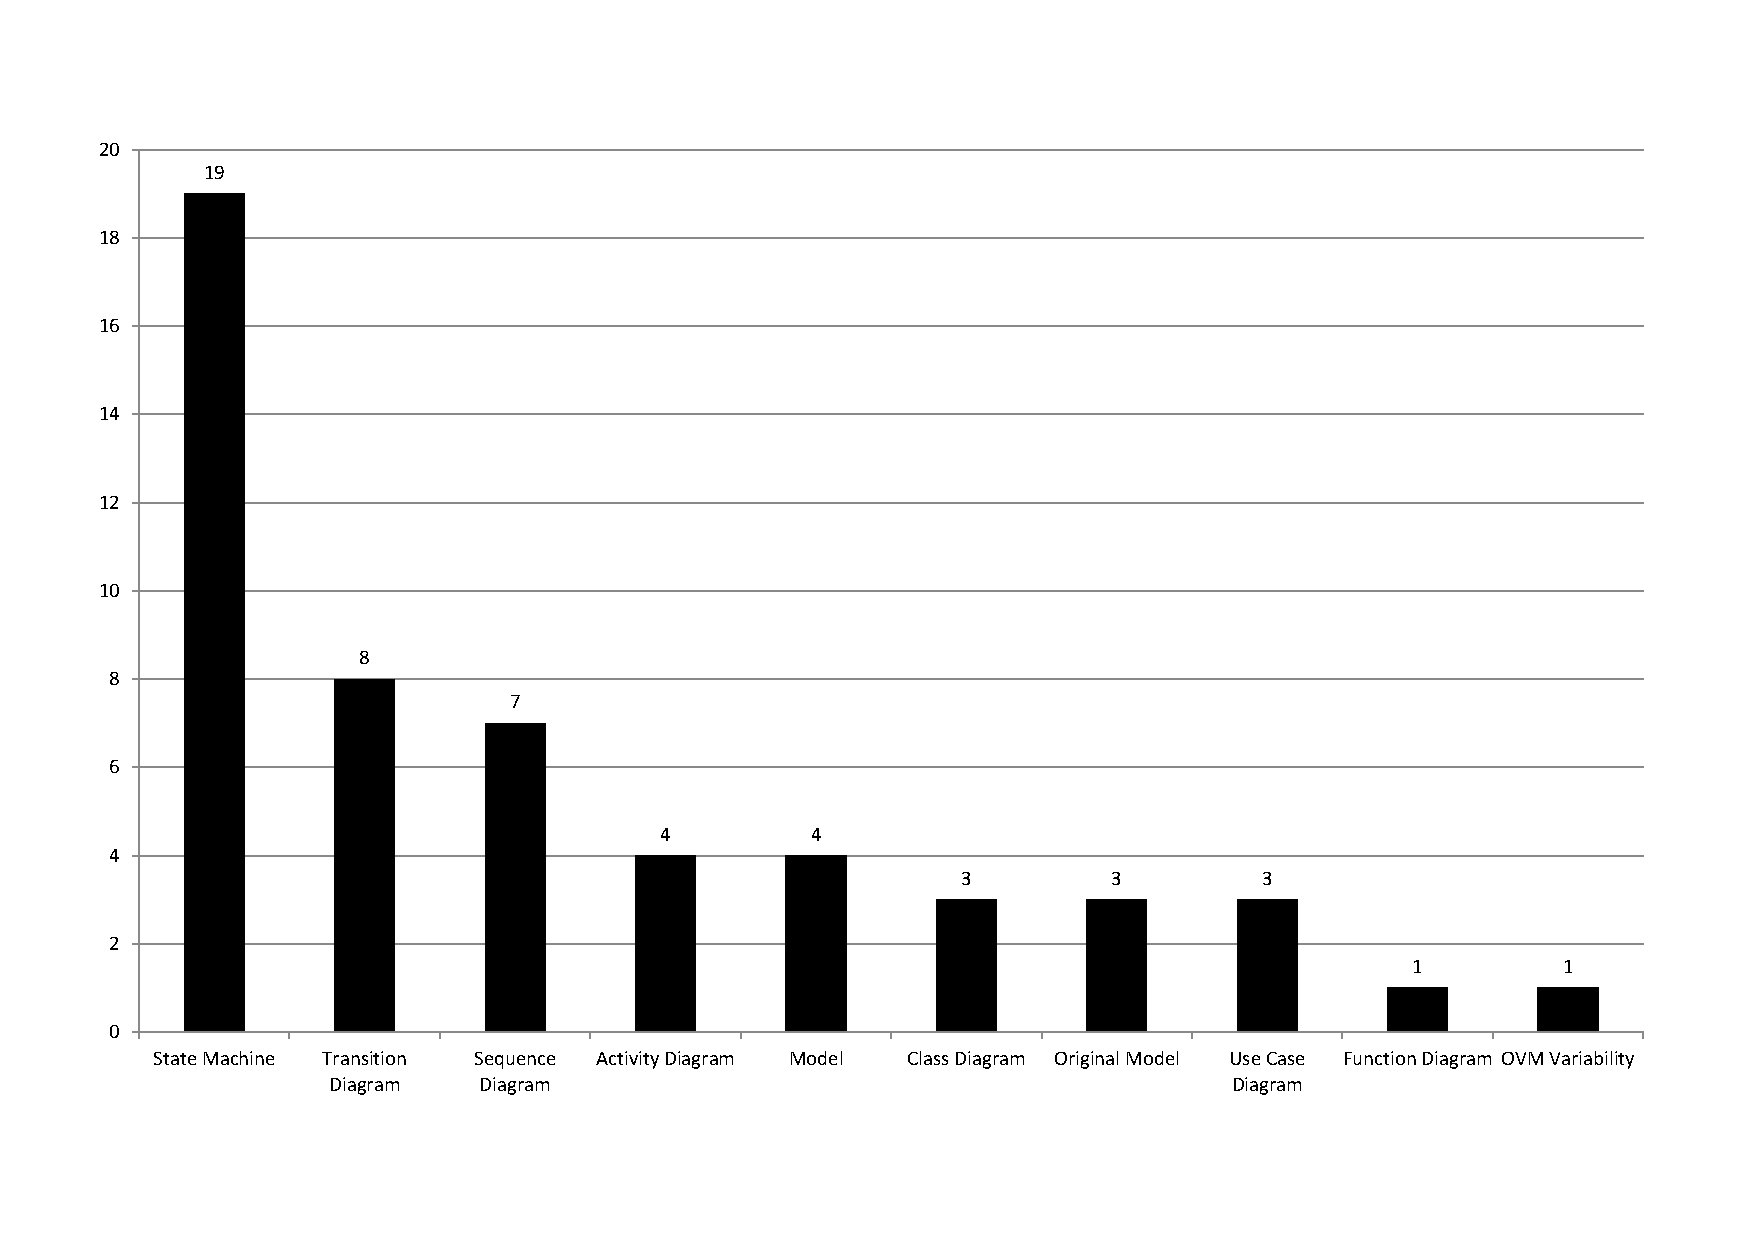
\includegraphics[scale=0.50]{chart_artifacts.pdf}
	\caption{Automação TBM para LPS de abordagens de teste}
	\label{fig:chart_artifacts}
\end{figure}

Alguns desses artefatos desempenham o papel do artefato original (inicial) em teste, que são os artefatos dos quais os casos de teste devem ser gerados. Outros artefatos são usados como elementos intermediários para fornecer ao TBM um meio de testar um determinado modelo original.


\paragraph{\textbf{Ferramentas usadas}}

\ref{fig:artefatoxlevelxmodel} apresenta ferramentas usadas para executar TBMs de LPSs relacionadas a artefatos. Algumas dessas ferramentas são mais frequentes, pois são usadas em mais de um estudo.

Podemos citar algumas ferramentas com um número maior de citações, como a série Rational IBM, o gerenciador de linha de produtos MaTeLo, variantes PURE, ferramentas CADeT e Eclipse \cite{olimpiew2005model, samih2014mplm, Lity_et_al2012, beohar2014spinal, costa2016split}.

As ferramentas CADeT \cite{olimpiew2005model} ajudam na geração de casos de teste a partir de modelos, bem como na especificação de casos de teste reutilizáveis. Fazendo uso do Delta para extrair os casos de teste com foco em regressão, esta ferramenta, bem como as ferramentas IBM Rational, Eclipse \cite{lochau2012incremental} e MoSo-PoLiTe foram consideradas para resolver o mesmo problema.


\begin{center}
	\begin{tiny}
		\begin{landscape}
			\begin{longtable}[c]{l|c|c|c|c|c|c|c|c|c}
				\caption{Comparação de ferramentas e artefatos primários ou secundários}
				\label{tab:artefatosXferramentas}\\
				\hline
				\textbf{Ferramenta}   & \textbf{\begin{tabular}[c]{@{}c@{}}Máquinas\\de Estado\end{tabular}} & \textbf{\begin{tabular}[c]{@{}c@{}}Direto \\do\\Modelo\end{tabular}} & \textbf{\begin{tabular}[c]{@{}c@{}}Diagrama\\de Classe\end{tabular}} & \textbf{Statechart} & \textbf{\begin{tabular}[c]{@{}c@{}}Diagrama\\de Atividade\end{tabular}} & \textbf{\begin{tabular}[c]{@{}c@{}}Diagrama\\de Sequência\end{tabular}} & \textbf{\begin{tabular}[c]{@{}c@{}}Diagrama\\de Transição\end{tabular}} & \textbf{\begin{tabular}[c]{@{}c@{}}Diagrama\\de Funcionalidade\end{tabular}} & \textbf{Caso de Uso} \\\hline
				\endhead
				%
				\textbf{\begin{tabular}[c]{@{}l@{}}IBM Rational \\Rhapsody \end{tabular}}   & \checkmark  & & & & & & & & \\\hline
				\textbf{MoSo-PoLiTe}   &  & \checkmark &  & \checkmark &  &  &  &  &  \\\hline
				\textbf{\begin{tabular}[c]{@{}l@{}}MaTeLo Product \\Line Manager\end{tabular}}   &  & \checkmark &  &  &  &  &  &  &  \\\hline
				\textbf{LPSOT tool}   &  & \checkmark &  &  &  &  &  & \checkmark &  \\\hline
				\textbf{LPSTestbench}   &\checkmark  &  &  &  &  &  &  &  &  \\\hline
				\textbf{PURE variantes}   &\checkmark  &  & \checkmark & \checkmark &  &  &  &  &  \\\hline
				\textbf{UML2 Eclipse}   & \checkmark &  &  &  &  &  &  &  &  \\\hline
				\textbf{CVL-Too}   & \checkmark &  &  &  &  &  &  &  &  \\\hline
				\textbf{\begin{tabular}[c]{@{}l@{}}Rational Software\\Architect\end{tabular}} &  \checkmark  &  & \checkmark &  &  &  &  &  &  \\\hline
				\textbf{MOFLON - SDM} &    & \checkmark &  &  &  &  &  &  &  \\\hline
				\textbf{Rhapsody} &  &    &  & \checkmark &  &  &  &  &  \\\hline
				\textbf{CADeT Tools}   &  &  &  &  &\checkmark  &  &  &  &  \\\hline
				\textbf{TRUST tool}   &\checkmark  &  &  &  &  &  &  &  &  \\\hline
				\textbf{Selenium}  &  &  &  &  &  &  &  &  & \checkmark \\\hline
				\textbf{AspectOPTIMA}   &  &  &  &  &  &  &  & \checkmark &  \\\hline
				\textbf{Quick Test Pro}   &  &  &  &  &  &  &  &  & \checkmark \\\hline
				\textbf{\begin{tabular}[c]{@{}l@{}}Rational \\Functional Tester\end{tabular}}   &  &  &  &  &  &  &  &  & \checkmark \\\hline
				\textbf{Pralíntool}   &  &  & \checkmark &  &  &\checkmark  &  &  &  \\\hline
				\textbf{VIBeS} &  \checkmark  &  &  &  &  &  &  &  &  \\\hline
				\textbf{Eclipse}   & \checkmark &  &  &  &  & \checkmark &  &  &  \\\hline
				\textbf{UML2 Tools}   &  &  &  &  &  & \checkmark &  &  &  \\\hline
				\textbf{ViTAL} &    &  &  &  &  &  & \checkmark &  &  \\\hline
				\textbf{visio} &  \checkmark  &  &  &  &  &  &  &  &  \\\hline
				\textbf{ATG} &  \checkmark  &  &  &  &  &  &  &  &  \\\hline
				\textbf{Excel}   & \checkmark &  &  &  &  &  &  &  &  \\\hline
			\end{longtable}
		\end{landscape}
	\end{tiny}	
\end{center}

\paragraph{\textbf{Modelos LPS}}

Quanto ao tipo de modelo de LPS considerado entre os trabalhos analisados, a maioria foi feita usando \textit{Behavioral-based}, que se caracteriza por ser comportamental, talvez a razão para isso, seja porque os modelos são ricos em detalhes, facilitando interpretação ou configuração, mesmo se o modelo é posteriormente convertido em um artefato, primário ou intermediário. Na \ref{table:cenario} pode-se observar que vários trabalhos utilizam o modelo de modelos baseados em Cenário, a relação se deve ao fato de estes trabalhos fazerem uso de artefatos intermediários, trabalhando com cenários de uso ao invés de comportamento direto.

\begin{table}[!h]
	\centering
	\scriptsize
	\caption{TBM de LPS Tipos de Modelos}
	\label{table:cenario}
	\begin{tabular}{l|l|c}
		\hline
		
		\textbf{Modelo LPS Considerado} & \textbf{Referência} &  \textbf{Estudos} \\\hline \hline
		
		Scenario-based & \begin{tabular}[c]{@{}l@{}} S3, S11, S19, S20, S24, S31, S38, S40, S41,\\S42, S43, S44\end{tabular} & 12 \\\hline
		
		Class-oriented & S6 & 01 \\\hline
		
		Behavioral-based & \begin{tabular}[c]{@{}l@{}} S1, S2, S4, S7, S8, S9, S10, S12, S13, S14,\\S15, S16, S17, S18, S21, S22, S23, S25,\\S26, S27, S28, S29, S30, S33, S34, S35, S36,\\S37, S39\end{tabular} & 29 \\\hline
		
		Não Identificado 	& S5, S32 & 02 \\\hline \hline
		
		\multicolumn{2}{c|}{\textbf{TOTAL}} & \textbf{44} \\\hline
	\end{tabular}
\end{table}


\begin{landscape}
	\begin{figure}[!h]	
		\centering
		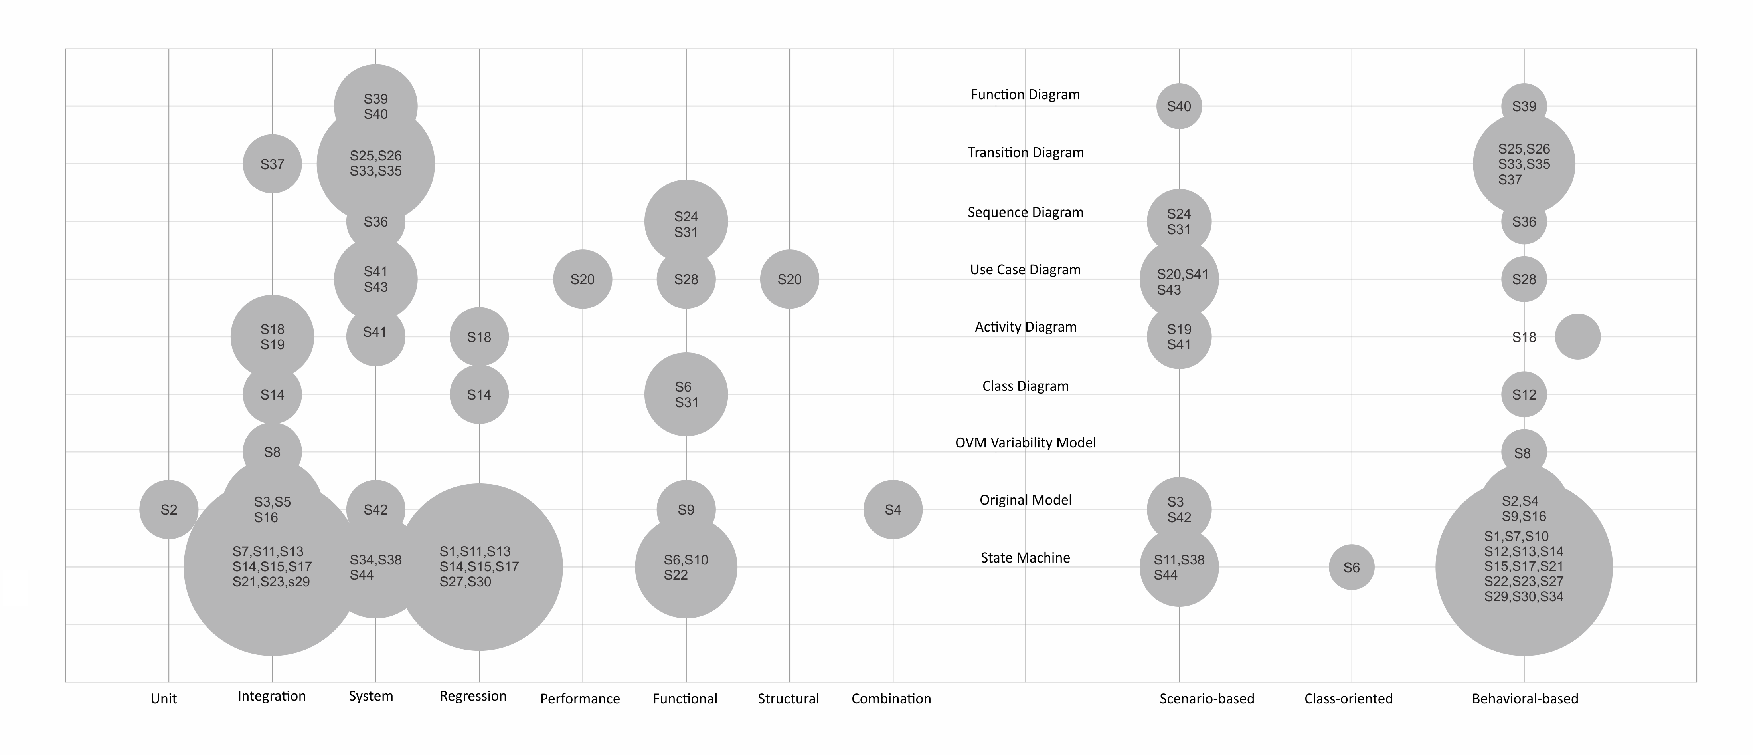
\includegraphics[scale=0.85]{artefatoXlevelsXmodels.pdf}
		\caption{Artefatos X Níveis X Modelos}
		\label{fig:artefatoxlevelxmodel}
	\end{figure}
\end{landscape}

\subsubsection{\bf{RQ.3:Como a variabilidade e o tempo de ligação são tratados durante o TBM de LPSs?}}

Como a variabilidade é a essência da LPS, assim como é diretamente relacionada ao tempo de vinculação, nesta seção apresentamos resultados nos quais os estudos levam em conta tais conceitos e como eles os tratam.

\ref{tab:variability_treatment} classifica os estudos que:consideram a variabilidade (linha \textit{`` Sim ''}) durante o TBM do LPS e não consideram a variabilidade (linha \textit{`` Não ''}). Em vários estudos, não conseguimos identificar se as variabilidades são tratadas.

\begin{table}[!h]
	\centering
	\scriptsize
	\caption{Estudos que tratam da variabilidade durante as atividades da TBM}
	\label{tab:variability_treatment}
	\begin{tabular}{l|l|c}
		\hline
		\textbf{Trata a variabilidade?} & \textbf{ID do Estudo} & \textbf{Estudos} \\\hline \hline
		
		Sim & \begin{tabular}[c]{@{}l@{}} S1, S2, S4, S5, S6, S7, S8, S9, S10, S12, S13, S14, S15,\\S16, S17, S18, S19, S21, S22, S24, S25, S27, S28, S29, \\S30, S31, S33, S34, S37, S40\end{tabular} & 30\\\hline
		
		Não & S39, S43 & 02\\\hline
		
		Não Identificado & \begin{tabular}[c]{@{}l@{}} S3, S11, S20, S23, S26, S32, S35, S36, S38, S41, S42, S44\end{tabular} & 12 \\\hline \hline
		
		\multicolumn{2}{c|}{\textbf{TOTAL}} & \textbf{44} \\\hline
	\end{tabular}
\end{table}

Apenas dois estudos (S39, S43) não tratam a variabilidade durante atividades de TBM. Isso ocorre porque eles aplicam testes em produtos específicos de LPS na engenharia de aplicativos.

Como podemos observar na \ref{tab:variability_treatment}, 68,1 \% (30/44) dos estudos tratam a variabilidade durante qualquer atividade de TBM de LPSs. 

Muitas estratégias diferentes são usadas para lidar com a variabilidade durante o TBM. A variabilidade pode ser modelada e resolvida em diagramas UML, com a geração de diagramas de classes e máquinas de estados \cite{wang2013automated} a serem testadas. 

Idiomas específicos também podem ser usados para especificar a variabilidade dos casos de teste \cite{devroey2014behavioural}. A \ref{fig:typexvariability} resume quais estudos tratam ou não a variabilidade por tipo de solução. 

\begin{figure}[!h]
	\centering	
	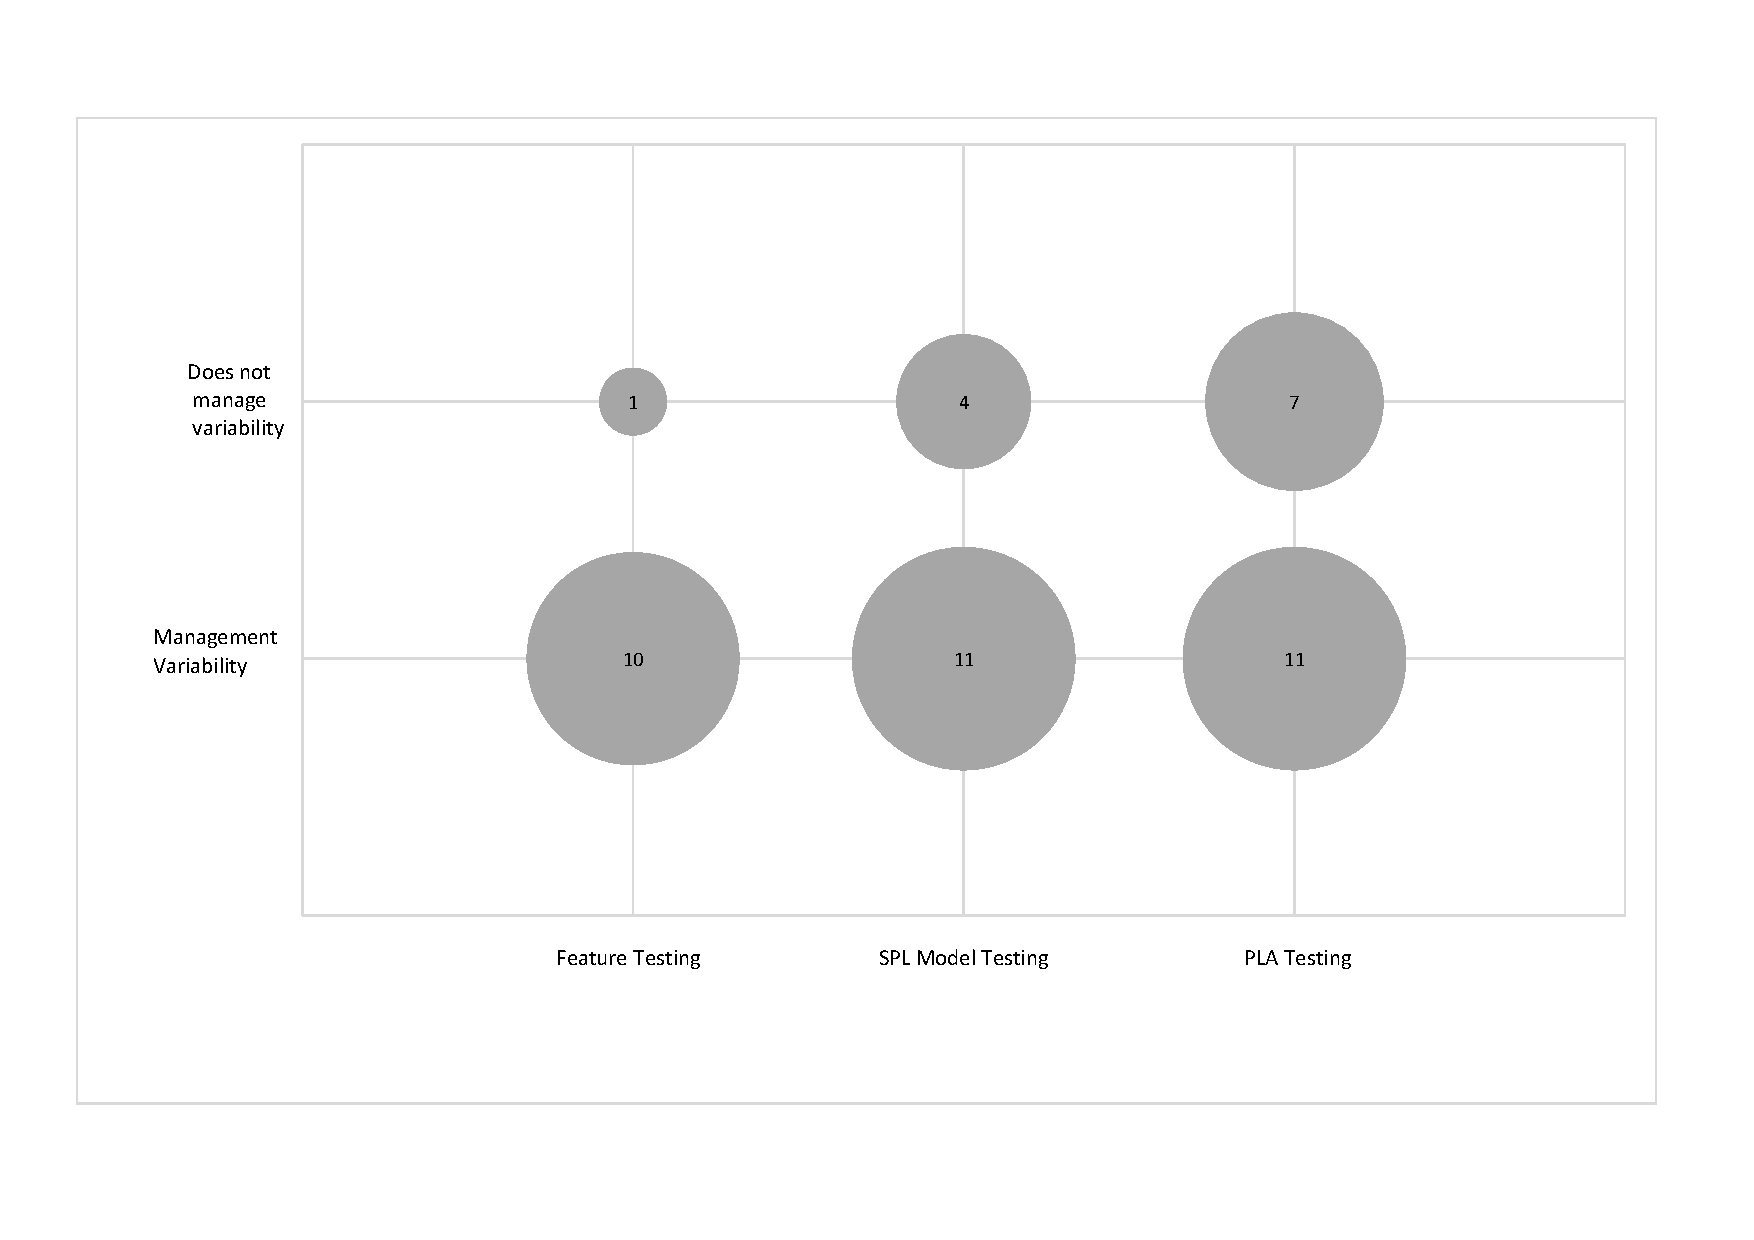
\includegraphics[scale=0.50]{bubble_typeXvariability.pdf}
	\caption{Tratamento da variabilidade por tipo de solução}
	\label{fig:typexvariability}
\end{figure}

O tempo de ligação é a capacidade de resolver a variabilidade em qualquer ponto do ciclo de vida do LPS. É obrigatório o aumento significativo dos níveis de variabilidade \cite{Chen_et_al2009}.

O tempo de vinculação no LPS é tradicionalmente em tempo de design, pré-compilação, compilação ou tempo de vinculação, lidando com a variabilidade estática. Já nos sistemas que lidam com a variabilidade dinâmica, pode ser em tempo de carregamento quando um sistema é implementado e carregado na memória e, em tempo de execução, após o sistema ter iniciado a execução de \cite{Alves_et_al2009}.

\ref{tab:bindingtime} lista estudos dos quais 86.3 \% (38/44) lidam com a variabilidade de vinculação em tempo de design. Os estudos restantes não informam seus tempos de ligação.

\begin{table}[!h]
	\centering
	\scriptsize
	\caption{Tempo de Ligação de Variabilidade em TBM de LPS}
	\label{tab:bindingtime}
	\begin{tabular}{l|l|c}
		\hline 
		
		\textbf{Binding Time} & \textbf{Id do Estudo}  &  \textbf{Estudos} \\\hline \hline
		
		Design Time & \begin{tabular}[c]{@{}l@{}} S7, S8, S9, S10, S11, S12, S13, S14, S15, S16, S17, S18,\\S19, S20, S21, S22, S23, S24, S25, S26, S27, S28, S29,\\S30, S31, S32, S33, S34, S35, S36, S37, S38, S39, S40,\\S41, S42, S43, S44\end{tabular} & 38 \\\hline
		
		Não Identificado & S1, S2, S3, S4, S5, S6 & 06 \\\hline \hline
		
		\multicolumn{2}{c|}{\textbf{TOTAL}} & \textbf{44} \\\hline
	\end{tabular}
\end{table}



\subsubsection{\bf{RQ.4:O TBM suporta testes de requisitos não funcionais do LPS?}}

Nenhum dos 44 estudos selecionados deste MSL apresenta ou menciona qualquer tipo de teste de requisitos de LPS não funcional. Embora o LPS e os produtos testados estejam geralmente em tempo de design, nada impede a criação dos requisitos não funcionais do plano de teste \cite{Lee_et_al2012}.

\citet{Feng_et_al2007} e \citet{Reis_et_al2007}, por exemplo, propõe a criação de casos de teste para a variabilidade considerando requisitos não-funcionais. 
\cite{Kakarontzas_et_al2008} propõe casos de teste hierárquicos para requisitos não funcionais específicos.

\subsubsection{\bf{RQ.5:Como as propostas de TBM de LPS são avaliadas?}}

Analisamos a avaliação da proposta de estudos de TBM de LPS com base no tipo de avaliação e no ambiente em que as avaliações são realizadas.

\ref{tab:coletaevidencia} lista estudos de acordo com seus tipos de avaliação, que são:\textit{Experiment} e \textit{Case Study}. Dos estudos selecionados, 79,5 \% (35/44) deles realizaram um desses tipos de avaliação. Em nove estudos, nem a avaliação foi realizada nem eles puderam ser identificados.

\begin{table}[!h]
	\centering
	\scriptsize
	\caption{Método de Evidenciação da Solução TBM para LPS}
	\label{tab:coletaevidencia}
	\begin{tabular}{l|l|c}
		\hline
		
		\textbf{Método de avaliação} & \textbf{ID do Estudo}  & \textbf{Estudos} \\\hline \hline
		
		Experimento & \begin{tabular}[c]{@{}l@{}} S1, S3, S4, S16, S20, S21, S23, S24, S25, S28, S39, S40,\\S42\end{tabular} &  13\\\hline
		
		Estudo de Caso & \begin{tabular}[c]{@{}l@{}} S2, S6, S7, S8, S9, S10, S11, S12, S13, S14, S15, S17,\\S19, S22, S26, S27, S29, S30, S33, S38, S43, S44\end{tabular} & 22 \\\hline
		
		Não Informado & S5, S18, S31, S32, S34, S35, S36, S37, S41 & 09 \\\hline \hline
		
		\multicolumn{2}{c|}{\textbf{TOTAL}} & \textbf{44} \\\hline
	\end{tabular}
\end{table}

Os experimentos são responsáveis por 29,5 \% (13/44) das avaliações realizadas. Nós não percebemos qualquer replicação experimental como um meio de impor resultados originais em uma determinada proposta. Além disso, poucos trabalhos apresentam elementos experimentais essenciais, como validade do estudo, perfil dos participantes, formulação e teste de hipóteses. Embora a maioria dos estudos relacionados à indústria não use participantes humanos, o tamanho da amostra não é relatado na maioria dos estudos. Cerca de 60 \% dos estudos disponibilizam seu pacote experimental ou parte dele, incluindo, por exemplo, diagramas e algoritmos, por meio de uma URL pública. Não entanto, a maioria das URLs não está mais disponível . Acreditamos que isso ocorre porque a maioria das avaliações é realizada em conjuntos de setores (consulte \ref{tab:areadevalidacao}).

Os estudos de caso são o tipo de avaliação mais realizado das propostas de TBM para LPS, com 50 \% (22/44) dos estudos e podem ter questões confidenciais.

Um aspecto importante relacionado à avaliação de propostas é o ambiente em que tais avaliações ocorrem. Portanto, analisamos quais estudos são realizados na academia e quais são realizados na indústria. \ref{tab:areadevalidacao} lista estudos por ambiente de avaliação.

\begin{table}[!h]
	\centering
	\scriptsize
	\caption{Ambientes de evidência de soluções TBM para LPS}
	\label{tab:areadevalidacao}
	\begin{tabular}{l|l|c}
		\hline
		
		\textbf{Environment} & \textbf{Study ID} &  \textbf{Count}\\\hline \hline
		
		Industria & \begin{tabular}[c]{@{}l@{}} S1, S2, S3, S4, S5, S6, S7, S8, S9, S10, S11, S12, S13,\\S14, S15, S16, S17, S20, S22, S29, S30, S38, S41, S42,\\S43, S44\end{tabular} & 26 \\\hline
		
		Academia & \begin{tabular}[c]{@{}l@{}} S19, S23, S24, S25, S26, S27, S28, S31, S32, S33, S34,\\S35, S36, S37, S39, S40\end{tabular} & 16 \\\hline
		
		Não Informado & S18, S21 & 02 \\\hline \hline
		
		\multicolumn{2}{c|}{\textbf{TOTAL}} & \textbf{44} \\\hline
	\end{tabular}
\end{table}

A maioria dos estudos ocorre na indústria, 59 \% (26/44), o que é de grande importância devido ao seu realismo e participação de profissionais de testes reais. Além disso, o conjunto da indústria fornece dados reais de projetos de LPS. Por outro lado, em estudos realizados em ambiente acadêmico, geralmente recruta os estudantes como participantes e usam NPSs pedagógicos ou não comerciais. Nãote que o uso de estudantes na engenharia de software baseada em evidências não é uma ameaça tão amplamente discutida \cite{Feldt_et_al2018}.

A \ref{fig:validacaoXlocal} mostra um gráfico de bolhas dos tipos de avaliação e seus ambientes.


\begin{figure}[!h]
	\centering
	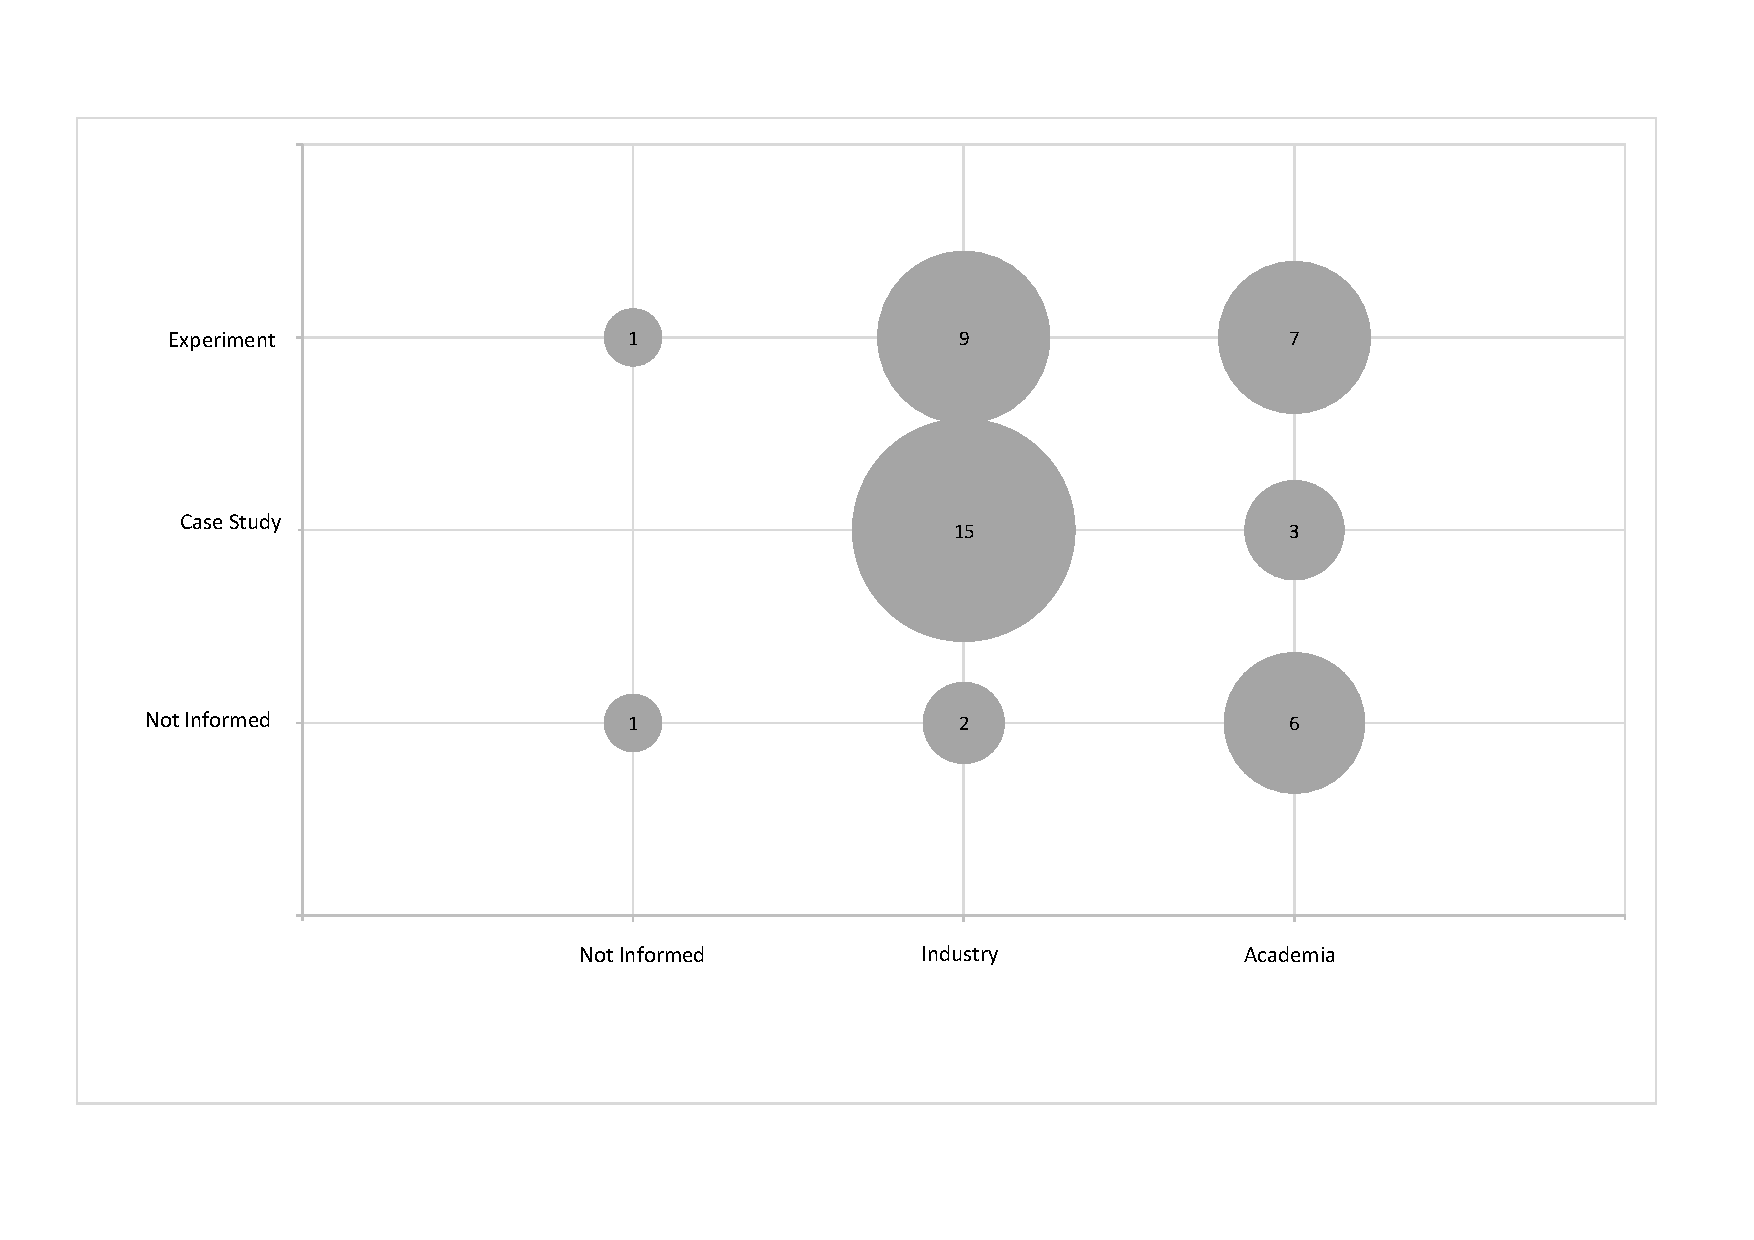
\includegraphics[scale=0.50]{validacaoXlocalIngles.pdf}
	\caption{Tipos de Avaliação de Propostas e Ambientes}
	\label{fig:validacaoXlocal}
\end{figure}

Como podemos observar na \ref{fig:validacaoXlocal}, a maioria dos estudos, nove experimentos e 15 estudos de caso, foram avaliados no conjunto da indústria, o que contribui para aumentar a confiabilidade das evidências das propostas fornecidas.



\subsubsection{\bf{RQ.6:Como a rastreabilidade é considerada durante atividades de TBM para LPSs?}}

A rastreabilidade ainda é uma das muitas lacunas de pesquisa no desenvolvimento de software, especialmente para LPSs. Como a rastreabilidade é responsável por identificar elementos importantes para derivar produtos específicos de LPS e para a evolução do LPS, é diretamente necessário durante as atividades do TBM \cite{Bernardino_et_al2017, costa2016split}. Além disso, a rastreabilidade fornece suporte essencial para garantia de qualidade de LPSs.

Nesta seção, analisamos quais estudos levam em consideração qualquer tipo de rastreabilidade durante as atividades de TBM. Assim, \ref{table:rastreabilidade} lista os estudos e se fornecem algum suporte para a rastreabilidade.

\begin{table}[!h]
	\centering
	\scriptsize
	\caption{Estudos com Suporte de Rastreabilidade para TBM de LPSs}
	\label{table:rastreabilidade}
	
	\begin{tabular}{l|l|c}
		\hline
		
		\textbf{\begin{tabular}[c]{@{}l@{}}Suporte\\a Rastreabilidade?\end{tabular}} & \textbf{ID do estudo}  & \textbf{Estudos}\\\hline \hline
		
		Sim & S5, S7, S15, S16, S17, S19, S20, S24, S31, S36, S37, S41 & 12 \\\hline
		
		Não & \begin{tabular}[c]{@{}l@{}} S1, S2, S3, S4, S6, S8, S9, S10, S11, S12, S13, S14, S18, S21,\\S22, S23, S25, S26, S27, S28, S29, S30, S32, S33, S34, S35,\\S38, S39, S40, S42, S43, S44 \end{tabular} & 32 \\\hline \hline
		
		\multicolumn{2}{c|}{\textbf{TOTAL}} & \textbf{44} \\\hline
	\end{tabular}
\end{table}

Poucos estudos (12/44) relatam ou mencionam a rastreabilidade como suporte. Além disso, nenhum deles declara como eles usam ou tratam a rastreabilidade. Eles só alegam que a rastreabilidade é fundamental para a geração de casos de teste, que devem ser o mais automatizados possível.


\subsection{Procedimentos de compartilhamento de dados do MSL}

Realizamos procedimentos para promover a abertura e a reprodutibilidade deste estudo. Portanto, nós:

\begin{itemize}
	\item fornece um formato de arquivo CSV com dados de todos os estudos deste MSL;
	\item fornece um formato de arquivo de metadados CSV explicando o arquivo CSV dos estudos;
	\item fornece arquivos PDF para todas as figuras e gráficos deste documento;
	\item fornece o formato de arquivo TEX para todas as tabelas deste documento;
	\item fornece formato de arquivo BIBTEX e CSV com referências dos estudos da Lista Final para uso em diferentes ferramentas bibliográficas;
	\item Fornece item de dados (CSV, PDF, TEX, arquivos BibTeX) em um repositório confiável compartilhamento de dados público aberto e permanente, chamado Zenodo \footnote{\url{zenodo.org}}, sob DOI \url{xxxx / aaaa / zzzz }.
\end{itemize}

\section{TBM4LPS:um roteiro para testes baseados em modelos de pesquisa de LPSs}
\label{sec:roadmapmslfinal}

Esta seção apresenta um roteiro, denominado TBM4LPS, como resultado do mapeamento da Lista Final de estudos com relação às fases do processo de TBM para LPSs. Três fases são consideradas:Baseado em artefato, Gerenciamento e Verificação de Variabilidade e Execução de TBM.

A  \ref{fig:guiaestudo} mostra o TBM4LPS sobre como os estudos são divididos de acordo com as fases e atividades do TBM. Para ilustrar o readomap, duas rotas serão apresentadas:a primeira baseada principalmente em um estudo primário específico, guia os usuários do modelo de estudo até a geração de casos de teste; e o segundo, considerando as três fases e atividades do TBM para LPS, dando aos usuários estudos que suportam tais fases.

\begin{tiny}
	\begin{landscape}	
		\begin{figure}[!h]
			\centering
			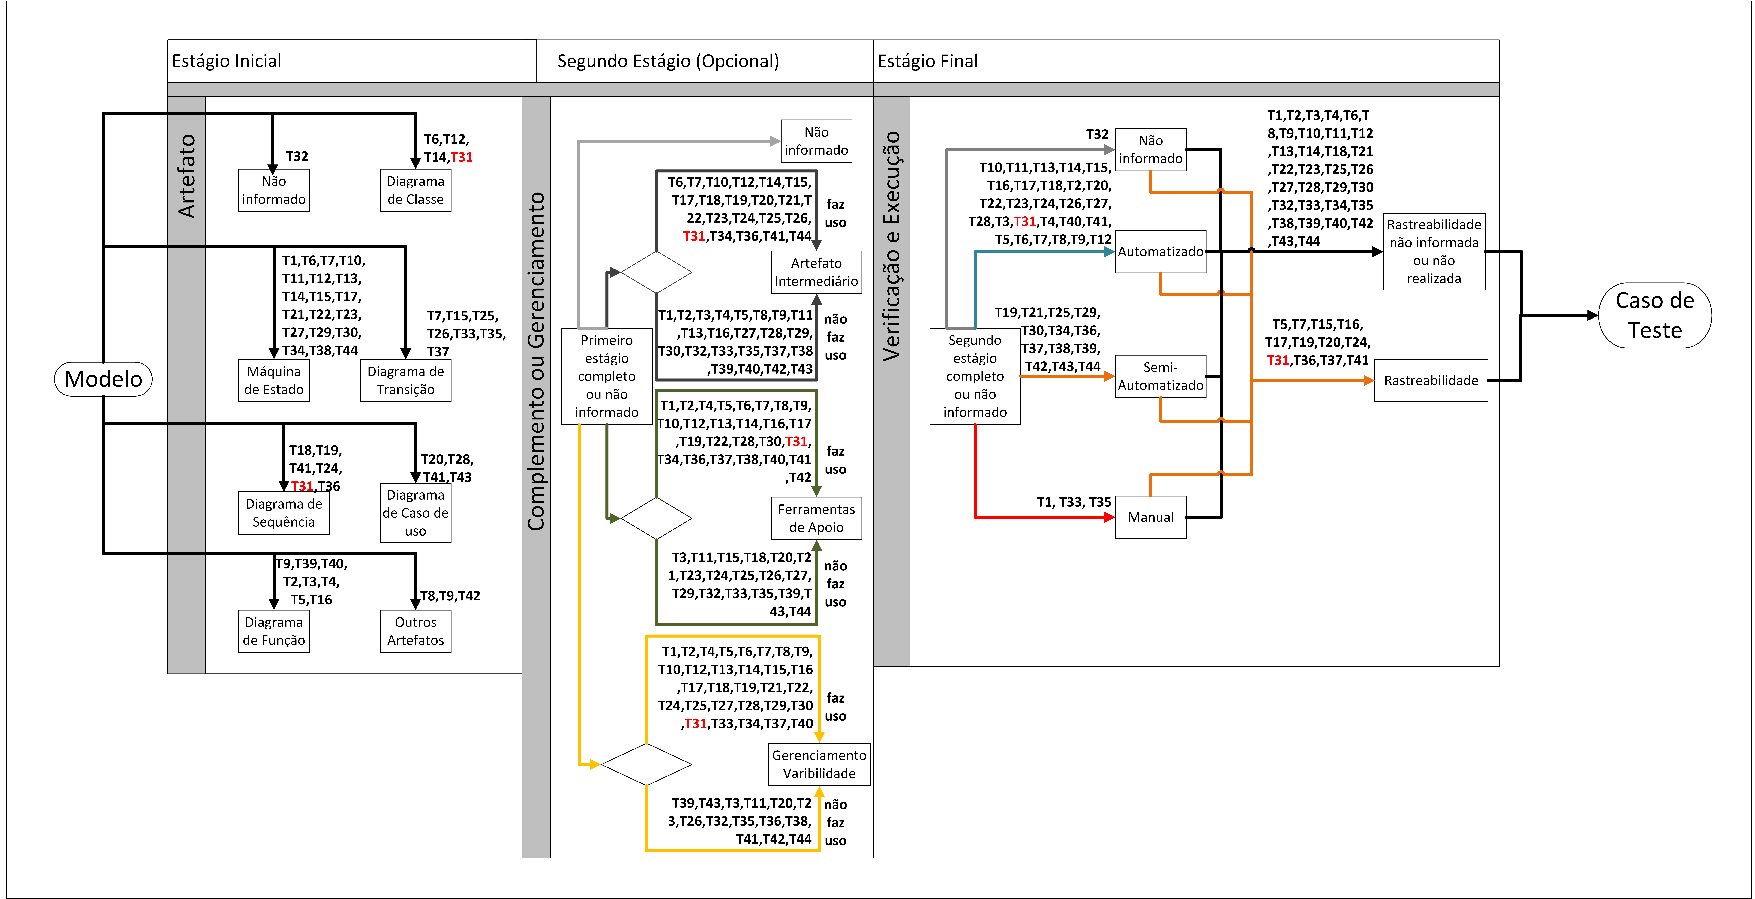
\includegraphics[scale=0.80]{guiaestudo.pdf}
			\caption{TBM4LPS: um roteiro de TBM para LPSs}
			\label{fig:guiaestudo}
		\end{figure}	
	\end{landscape}
\end{tiny}

As seções a seguir apresentam exemplos de aplicativos sobre como usar o TBM4LPS.

\subsection{Rota Primária Baseada no Estudo}

Digamos que, ao selecionar um estudo de \ref{table:listaextra} do seu ID, você queira verificar o \ref{fig:guiaestudo} qual caminho percorre, identificando seus estágios e atividades. Assim, inicialmente analisamos o primeiro estágio representado em \ref{fig:estagio1}, que é um excerto de \ref{fig:guiaestudo}.

\begin{figure}[!h]
	\centering
	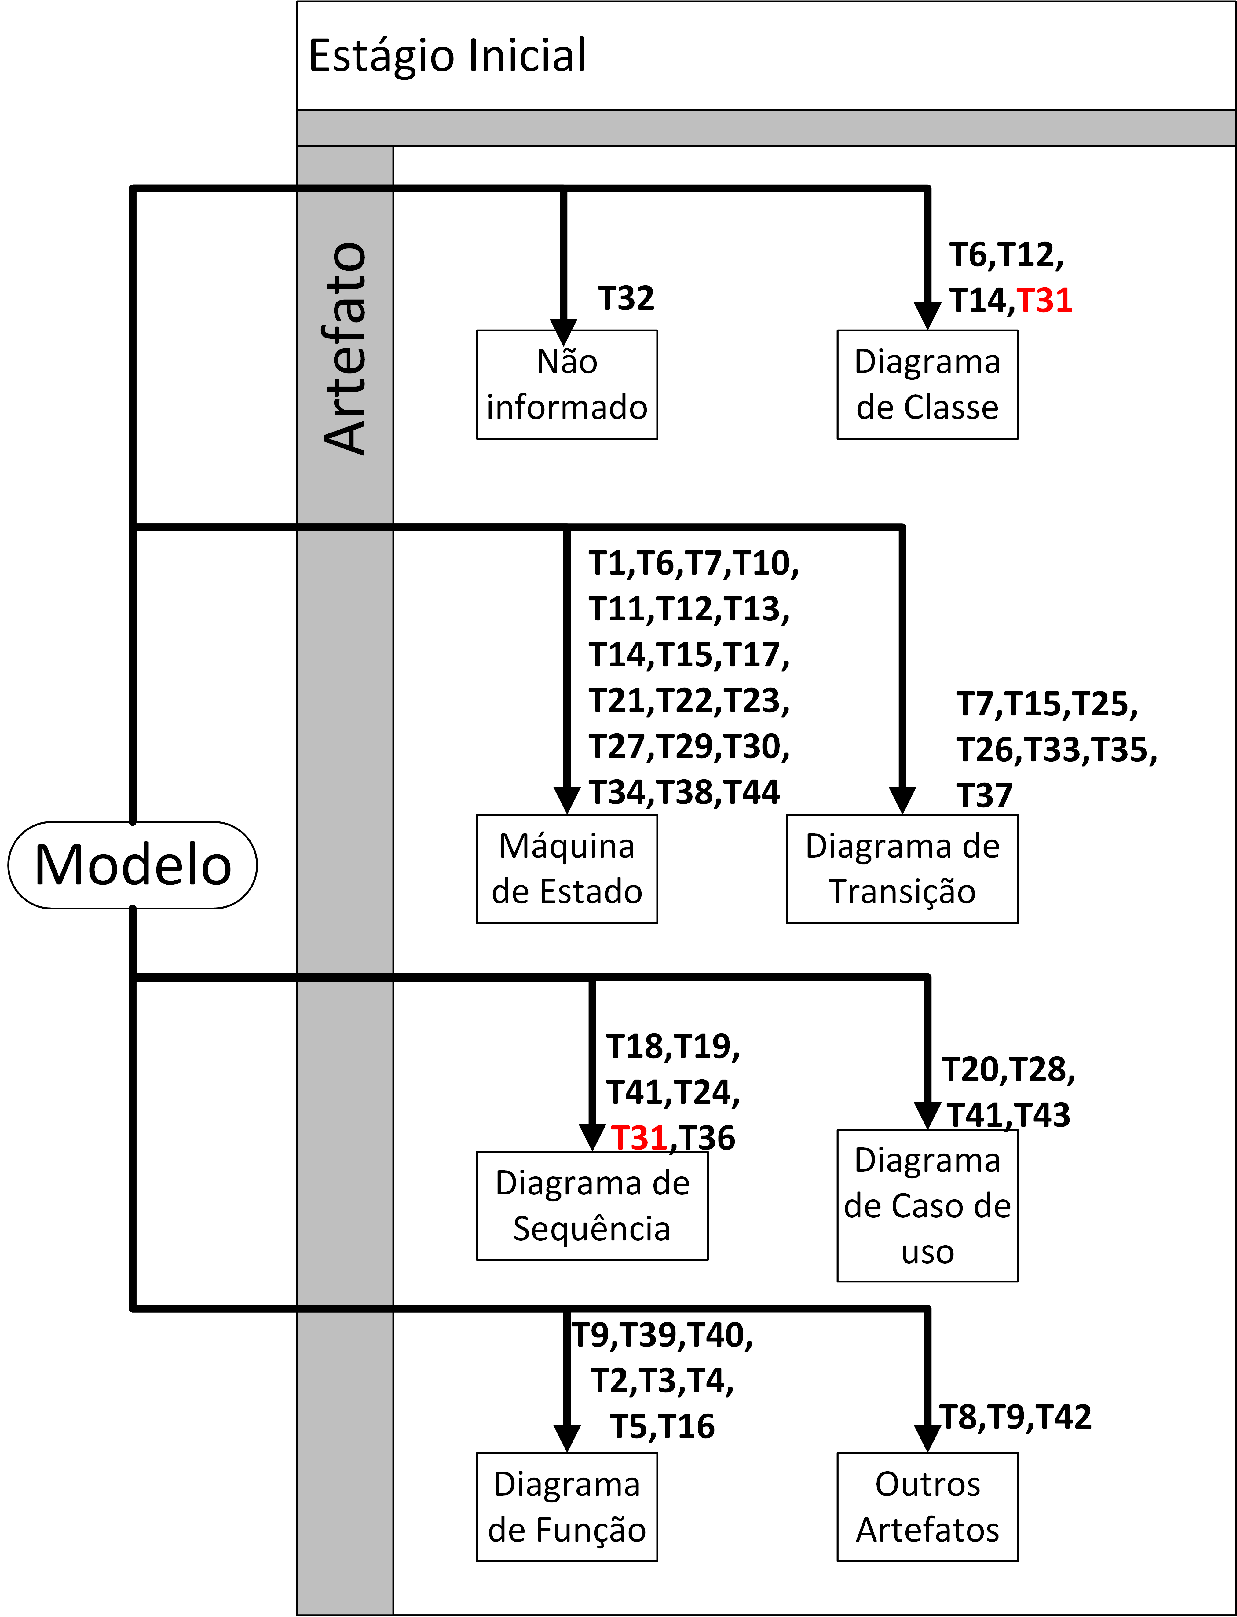
\includegraphics[scale=0.50]{estagioguia1.pdf}
	\caption{Etapa inicial, mostrando a localização do estudo T31}
	\label{fig:estagio1}
\end{figure}

Tomemos, por exemplo, o estudo T31. A partir de um modelo, o T31 faz uma conversão para o artefato do diagrama de sequência, então podemos considerar o T31. Com o estágio inicial concluído, o segundo estágio (opcional) é iniciado e o T31 considera o gerenciamento de variabilidade, suporte de ferramentas e geração de artefatos intermediários, pois nesse estágio abordamos o gerenciamento de variabilidade, uso de ferramentas, geração de artefatos intermediários e se não executar qualquer uma dessas atividades automaticamente, pode ser na geração do caso de teste.

\begin{figure}[!h]
	\centering
	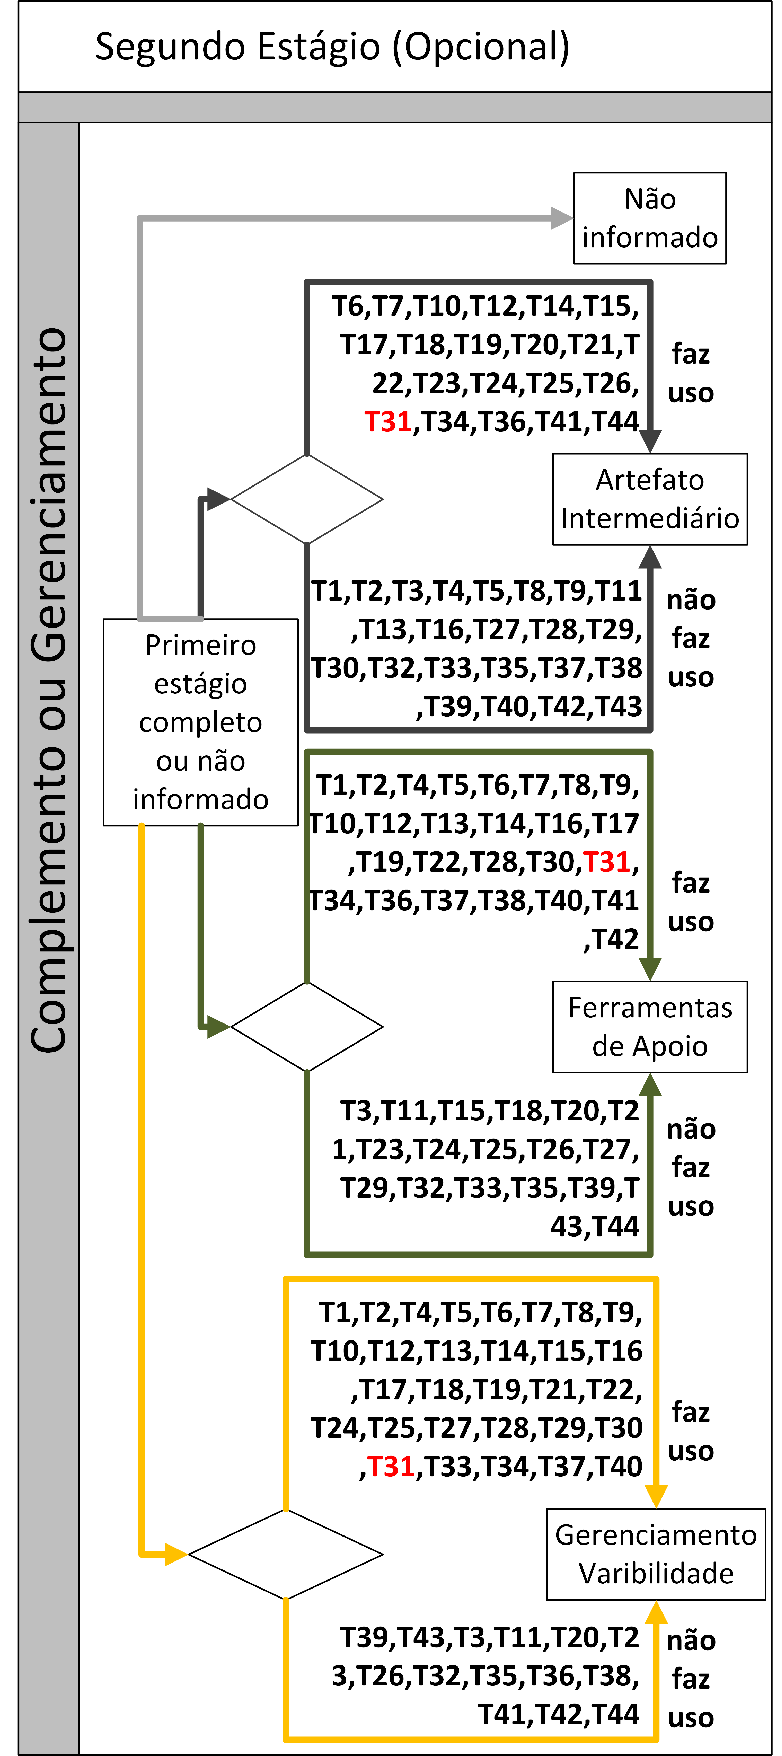
\includegraphics[scale=0.50]{estagioguia2.pdf}
	\caption{Segunda etapa, mostrando a localização do estudo T31}
	\label{fig:estagio2}
\end{figure}

\begin{figure}[!h]
	\centering
	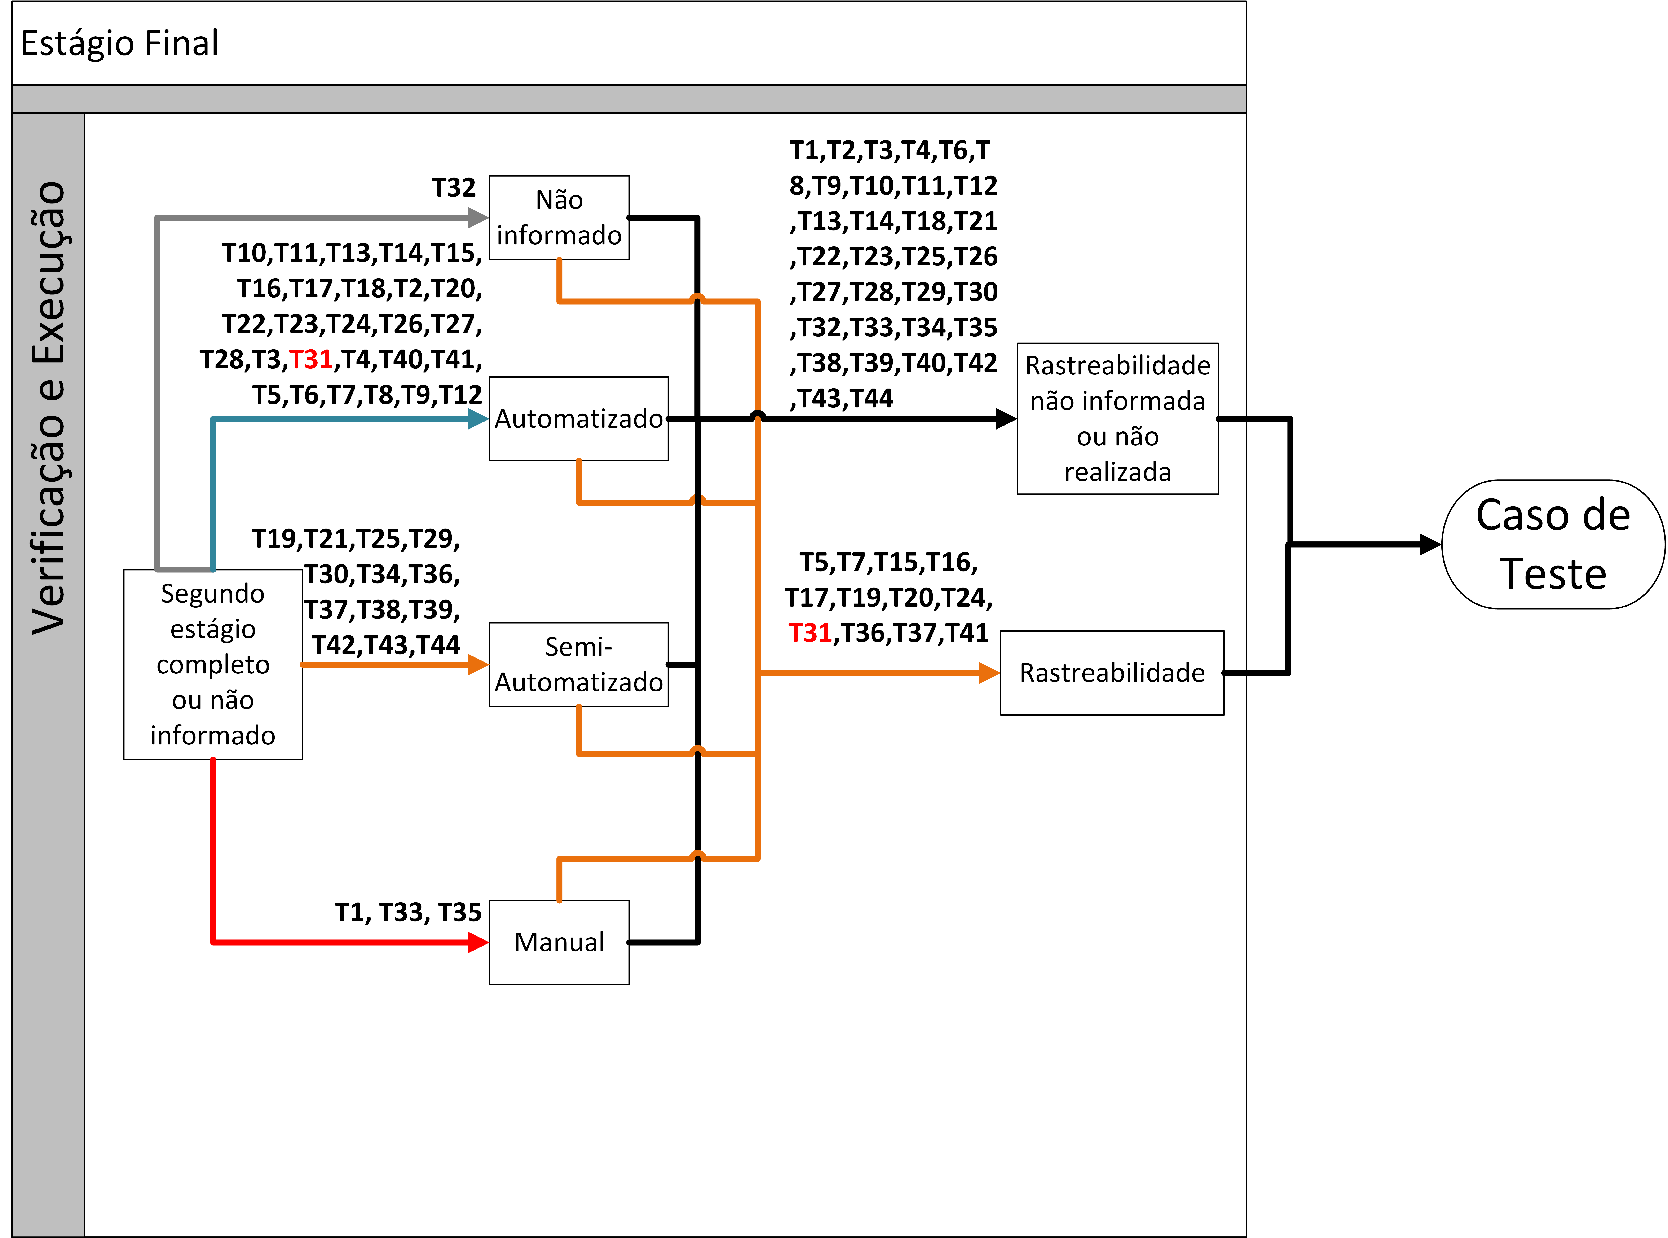
\includegraphics[scale=0.60]{estagioguia3.pdf}
	\caption{Etapa final mostrando a localização do estudo T31}
	\label{fig:estagio3}
\end{figure}

Ao apresentar o estágio final em \ref{fig:estagio3} pode-se analisar que o estudo T31 faz uso de processo automatizado e menciona a rastreabilidade. Isso conclui o curso do guia para o estudo T31, identificando, assim, quais etapas o estudo passou.

\subsection{Rota baseada em critérios}

O segundo cenário executa o tema TBM no LPS por assunto. Ao analisar o \ref{fig:estagio3}, por exemplo, pode-se verificar quais trabalhos fazem uso da rastreabilidade. Portanto, se o interesse do leitor é por obras que fazem uso da rastreabilidade, basta consultar essa atividade para obter a lista de tais obras.


\section{Observações Conclusivas}


Este mapeamento sistemático foi realizado para obter uma visão geral sobre testes baseados em modelo para linhas de software, e identificamos quarenta e quatro trabalhos publicados entre 2006 e 2016.
Há um desafio muito grande ao abordar o teste em LPS, onde os principais pontos levantados são o gerenciamento de variabilidade, a cobertura de erros, a automação de processos e a rastreabilidade.

O objetivo principal da pesquisa foi verificar se o TBM é aplicado no NPS e, quando aplicado, se o gerenciamento de variabilidade foi utilizado.
Após a análise dos dados extraídos do MSL, foi possível verificar e identificar as técnicas de teste de TBM utilizadas, que utilizam a notação UML, os trabalhos que realizam um controle de variabilidade, bem como a menção de rastreabilidade. Além disso, como os casos de teste são gerados, manualmente ou automatizados.

As contribuições para o TBM em LPS não são tão detalhadas quanto esperávamos, o que exigiu um trabalho extra na interpretação dos dados extraídos. Os principais dados que o MSL apresenta como contribuição são os artefatos utilizados, as técnicas relatadas, o uso de ferramentas e o uso do gerenciamento de variabilidade.

Com esse MSL, podemos ver que o domínio de maior desempenho é o software, a grande maioria considera o uso da variabilidade e a maior parte das validações estão sendo realizadas no setor, isso mostra que há um crescente interesse no assunto, embora não podemos identificar por que a rastreabilidade e os testes de requisitos não funcionais não são explicitamente apresentados, estudos adicionais sobre esses dois temas podem nos dizer mais sobre isso.

Um dos principais pontos que é a gestão da variabilidade atrelada ao modelo em LPS foi apresentado por uma maioria significativa, isso demonstra que há uma crescente conscientização da qualidade dos produtos variantes oriundos de um produto principal.

Devido a esse crescente interesse, incentivamos a comunidade a continuar com novas pesquisas para testes baseados em modelo, a fim de apresentar dados sobre rastreabilidade, automação de processos, cobertura de erros e gerenciamento de variabilidade. Para estes parecem precisar de mais compreensão e avaliação.